\documentclass[12pt,a4paper,bibtotoc,]{book}

%\usepackage{fancyheadings}
%\pagestyle{fancy}
%\renewcommand{\sectionmark}[1]{\markboth{#1}{}}
%\renewcommand{\subsectionmark}[1]{\markright{#1}}
%\rfoot{\leftmark\\rightmark}

\newcommand{\clearemptydoublepage}{\newpage{\pagestyle{empty}\cleardoublepage}}

\usepackage[dvips]{graphicx} 
\usepackage{epsfig}
\usepackage{algorithmic}
\usepackage[plain]{algorithm}
%\usepackage{amsmath,amsfonts}
%\usepackage{mathrsfs}
\usepackage{subfigure}
\usepackage{theorem}
\usepackage{url}
\usepackage[british, german]{babel}
\usepackage{german}
\usepackage{wrapfig}
\usepackage{setspace} 
\doublespacing

% wegen deutschen Umlauten
\usepackage[ansinew]{inputenc}



\pagestyle{headings}

\graphicspath{{graphics/}}

%\paperwidth 18cm

\textheight 21.5cm
\textwidth 16cm
\oddsidemargin 0cm
\evensidemargin 0cm
\topmargin 2.5cm
\headsep 0.8cm

%\footskip 3.0cm

\renewcommand{\baselinestretch}{1.6}
\renewcommand{\textfraction}{0.0}
\renewcommand{\bottomfraction}{1.0}
\renewcommand{\topfraction}{1.0}

\theoremstyle{break}
\newtheorem{Definition}{Definition}[section]

\def\rz{\ifmmode{I\hskip -3pt R}
    \else{\hbox{$I\hskip -3pt R$}}\fi} %reelle Zahlen


\bibliographystyle{unsrt}

\floatstyle{ruled}
\newfloat{program}{thp}{lop}
\floatname{program}{Programm}

\begin{document}


\frontmatter
\thispagestyle{empty}
\topmargin 0.8cm

\begin{center}
~
\vspace{0cm}

{\large \textbf{DIPLOMARBEIT}}

\vspace{1.8cm}
\parbox{0.9\textwidth}{
  \begin{center}
    \large \textbf{%
		XCS in dynamischen Multiagenten-�berwachungsszenarios \\ [1.2ex]
		ohne globaler Kommunikation
      }
  \end{center}
  }

\vspace{1.1cm}

{\fontsize{11pt}{12} \selectfont%
  von
}
\vspace{0.8cm}

{\fontsize{12pt}{12} \selectfont%
  \textbf{Clemens Lode}
}

\vspace{3cm}


{\fontsize{12pt}{12} \selectfont%
  \textbf{Institut f�r Angewandte Informatik\\
	 und Formale Beschreibungsverfahren}
}\\
%\vspace{1cm}

{\fontsize{12pt}{12} \selectfont%
  \textbf{Universit�t Karlsruhe}
}\\

\vspace{1cm}


\textbf{Referent: Prof. Dr. Hartmut Schmeck}\\
\textbf{Betreuer: Dipl. Wi-Inf. Urban Richter}

\vspace{2cm}
\textbf{Karlsruhe, 30.03.2009}


\end{center}



 
\tableofcontents
\clearemptydoublepage
\listoffigures
\clearemptydoublepage
\listoftables
\clearemptydoublepage
\pagestyle{plain}
\include{preface}
\clearemptydoublepage
\pagestyle{headings}
\mainmatter

\chapter{Einf�hrung}\label{introduction:cha}

Ein aktuelles Forschungsgebiet aus dem Bereich der \emph{learning classifier systems} (LCS) stellen die sogenannten \emph{accuracy based} LCS (XCS) dar. In der Basis entspricht XCS einem LCS, d.h. eine Reihe von Regeln, bestehend jeweils aus einer Kondition und einer Aktion, werden mittels \emph{reinforcement learning} schrittweise bewertet und an eine Umwelt angepasst. Die Frage nach dem Zeitpunkt der Bewertung teilt die verwendeten Algorithmen bei XCS in \emph{single step} und \emph{multi step} Verfahren ein. Hauptaugenmerk dieser Arbeit soll das \emph{multi step} Verfahren sein, bei dem die Bewertung (der \emph{reward} der Regeln erst nach einigen Schritten verf�gbar ist und an zur�ckliegende Regeln sukzessive weitergeleitet wird, um m�glichst alle beteiligten Regeln an dem \emph{reward} zu beteiligen.\\

Bisherige Anwendungen haben sich haupts�chlich auf statische Szenarien mit nur einem XCS oder mit mehreren Agenten mit globaler Organisation und Kommunikation beschr�nkt. Diese Arbeit hat sich auf die Problemstellung konzentriert, wie man XCS modifizieren sollte, damit es ein dynamisches �berwachungsszenario, mit sich bewegendem Zielobjekt und mehreren Agenten, im Vergleich zu zuf�lliger Bewegung m�glichst gut bestehen.\\

Die Zahl der m�glichen Anpassungen, insbesondere was das Szenario, die XCS Parameter und Anpassungen an die XCS Implementierung betrifft, sind un�berschaubar gro� und bed�rfen in erster Linie einer theoretischen Basis, welche in diesem Bereich noch nicht weit fortgeschritten ist. Ziel dieser Arbeit soll es deshalb sein, zu untersuchen, welche Anpassungen speziell f�r das �berwachungsszenario erfolgsversprechend sind.\\

*Empirisch

Im Wesentlichen wurde hierzu in zwei Schritten vorgegangen, die auch in der Struktur der Arbeit wiedergespiegelt sind, um eine logische Kette aufzubauen. Der erste Schritt soll sich alleine um die Beschreibung des Problems und des Szenarios drehen. 
Literatur Szenarien, Woods Maze etc.

TODO 




Neben der Anpassung der Implementation, damit XCS f�r eine solche Problemstellung anwendbar ist, wurden weitere Modifikationen durchgef�hrt, die in einigen F�llen zu deutlich besseren Ergebnissen als die der Standardimplementation f�hrten.\\
Au�erdem wurde untersucht, wie eine einfache Kommunikation ohne globale Steuereinheit stattfinden kann, um das Ergebnis weiter zu verbessern. Im Wesentlichen war dazu eine weitere Anpassung von XCS vonn�ten, so dass die Implementierung auch mit (durch die Kommunikation) zeitverz�gerten und externen \emph{rewards} arbeiten konnte. Wesentliche Schlu�folgerung ist, dass sich unterschiedliche Szenarien unterschiedlich gut f�r Kommunikation eignen, dass Kommunikation M�glichkeiten zur Anpassung bietet, um mit einer variablen, unbekannten Feldgr��e besser zurecht zu kommen und, dass es Szenarien gibt, in denen Kommunikation signifikante Vorteile erbringt.\\
Erfolgversprechende Ansatzpunkte f�r weitere Forschung gibt es im Bereich der mathematischen Begr�ndung, warum die Implementierung Vorteile erbringt, im Ausbau der Untersuchung von Kommunikation zwischen den Agenten in Verbindung mit XCS und in der Anwendung der gefundenen Ergebnisse in anderen Problemstellungen �hnlicher Natur.

\chapter{Beschreibung des Szenarios}\label{scenario_description:cha}

Im Wesentlichen sollen die Algorithmen, die in dieser Arbeit besprochen werden, in einem Szenario getestet werden, in dem mehrere Agenten ein sich bewegendes Zielobjekt �berwachen sollen. Dies soll im folgenden als �berwachungsszenario bezeichnet werden. Die Qualit�t eines Algorithmus in einem solchen �berwachungsszenario wird anhand des Anteils der Zeit bewertet, in der er mit Hilfe der Agenten das Zielobjekt �berwachen konnte, relativ zur Gesamtzeit (siehe Kapitel~\ref{qualitaet:sec}).\\

Verwendetes Umfeld wird ein quadratischer Torus sein, der aus quadratischen Feldern besteht. Jedes bewegliche Objekt auf einem Feld des Torus kann sich in einem Zeitschritt nur auf eines der vier Nachbarfelder bewegen (mit Ausnahme des Zielobjekts, welches mehrere Bewegungen in einem Zeitschritt durchf�hren kann, N�heres dazu im Kapitel~\ref{base_properties_goal:sec}).\\
Die Felder k�nnen entweder leer oder durch ein Objekt besetzt sein. Besetzte Felder k�nnen nicht betreten werden, eine Bewegung auf ein solches Feld schl�gt ohne weitere Konsequenzen fehl.\\
Es gibt drei verschiedene Arten von Objekten: Unbewegliche Hindernisse, ein zu �berwachendes Zielobjekt und Agenten. Sowohl das Zielobjekt als auch die Agenten bewegen sich jeweils anhand eines bestimmten Algorithmus und bestimmter Sensordaten. Eine n�here Beschreibung der Agenten findet sich in Kapitel~\ref{agents:cha}, w�hrend die Eigenschaften des Zielobjekts in Kapitel~\ref{zielobjekt:cha} beschrieben wird.\\

Ziel dieses Kapitels wird vor allem sein, auf Kapitel~\ref{analysis_sans_lcs:cha} vorzubereiten, in dem anhand von Tests herausgefunden werden soll, welche der hier vorgestellten Szenarien brauchbare Ergebnisse liefern kann, um zum einen das gestellte Problem an sich, als auch die jeweils erforderlichen Eigenschaften besser verstehen zu k�nnen.\\

Eine separate Besch�ftigung mit diesen - relativ einfachen - Szenarien war notwendig, um zum einen das eigene Simulationsprogramm zu testen und zum anderen um vergleichbare Ergebnisse zu erhalten. Ein R�ckgriff auf die Literatur war deshalb nicht m�glich, insbesondere gibt es keine Arbeiten in Bezug auf XCS mit einer solchen Problemstellung. Zwar entspricht das Standardszenario bei XCS einem Feld, einem Agenten, Hindernissen und einem Ziel, es fehlen jedoch Arbeiten, in denen Sichtbarkeit (die Sichtweite beschr�nkte sich in der Literatur meist auf angrenzende Felder), Kollaboration (meist war nur ein einzelner Agenten Gegenstand der Untersuchung), Dynamik (meist gab es feste Start- und Zielpunkte) und die Messung der durchschnittlichen Qualit�t (meist ging es um die Anzahl der Schritte zum Ziel) gemeinsam in einem Szenario betrachtet werden.\\

Im folgenden sollen nun also auf diese einzelnen Punkte n�her eingegangen werden und eine Abgrenzung zu Arbeiten in der Literatur aufgezeigt werden.

\section{Definition einer Probleminstanz}\label{definition_probleminstanz:sec}

Eine einzelne Probleminstanz entspricht einem Torus mit einer bestimmten Anfangsbelegung mit bestimmten Objekten und bestimmten Parametern zur Sichtbarkeit. Die Anfangsbelegung ist �ber einen \emph{random seed} Wert bestimmt. Soweit nicht anders angegeben, sollen hier Prombleninstanzen der Gr��e 16x16 Felder betrachtet werden, insbesondere beziehen sich die Ergebnisse der Tests auf diesen Fall.\\
Jedes Problem soll sich, sofern nicht anders angegeben, �ber 500 Zeitschritte ziehen. Ein einzelnes Experiment entspricht dem Test einer Anzahl von Probleminstanzen, die jeweils mit einer Reihe von \emph{random seed} Werten initialisiert werden. In einem Durchlauf werden mehrere Experimente (jeweils mit unterschiedlichen Reihen an \emph{random seed} Werten) durchgef�hrt. Falls nicht anders angegeben sollen die Tests jeweils �ber 10 Experimente mit jeweils 10 Problemen laufen.\\

TODO XCS, neustart etc.

\section{Sichtbarkeit von Objekten}\label{sichtbarket:sec}

Der Parameter \emph{sight range} bzw. \emph{reward range} einer Probleminstanz bestimmt, bis zu welcher Distanz andere Objekte von einem Objekt als "`gesehen"' bzw. "`�berwacht"' gelten, sofern die Sicht durch andere Objekte nicht versperrt ist. Der Parameter \emph{reward range} ist relevant f�r die Bewertung der Qualit�t des Algorithmus (siehe Kapitel~\ref{qualitaet:sec}) und wird immer kleiner als der \emph{sight range} Wert gew�hlt. �ber die Sensoren kann ein Agent feststellen, ob sich Objekte in welcher der beiden Reichweiten befinden. Falls nicht anders angegeben sollen jeweils \emph{sight range} auf 5 und \emph{reward range} auf 2 gesetzt werden und in den Abbildungen jeweils der hellblaue Bereich den �berwachten und der hell- und dunkelblaue Bereich den gesehenen Bereich darstellen.


\section{Kollaboration}

Wesentliches Hauptaugenmerk der Gestaltung der Szenarien soll Kollaboration sein, d.h. die Aufgabe soll mit Hilfe mehrerer Agenten gemeinsam gel�st werden. 

TODO Literatur Definition vo Kollaboration in der Literatur, Abgrenzung

Eine erfolgreiche �berwachung soll deswegen so definiert sein, dass sich ein beliebiger Agent in �berwachungsreichweite des Zielobjekts befindet. Angesichts dessen, dass diese Aufgabe auch ein einzelner Agent erf�llen kann, sofern die Geschwindigkeit des Zielobjekts kleiner oder gleich der Geschwindigkeit des Agenten ist, sollen in sp�teren Tests (insbesondere in Kapitel~\ref{lcs_analysis:cha} beim Vergleich unterschiedlicher XCS Varianten und im Kapitel~\ref{cha:parameter} beim Vergleich unterschiedlicher XCS Parameter) unterschiedliche Geschwindigkeiten getestet werden.\\

Bewegt sich das Zielobjekt zu schnell, werden die Agenten Schwierigkeiten haben, einen Bezug zwischen Sensordaten und eigener Aktionen zu erkennen, bewegt es sich zu langsam, wird das Problem sehr einfach, eine einzelne Regel ("`Bewege dich auf das Ziel zu"`) w�rde zur L�sung dann schon gen�gen.\\

\section{Dynamik}

Die Szenarien fallen alle unter die Kategorie "`dynamisch"'. Darunter soll in diesem Zusammenhang verstanden werden, dass es kein festes Ziel gibt, das erreicht werden soll oder kann, das Zielobjekt befindet sich in stetiger Bewegung, wie auch sich andere Agenten in Bewegung befinden k�nnen.\\

Dies ist ein wesentlicher Gesichtspunkt, dass diese Arbeit von vielen anderen unterscheidet, Gegenstand der Untersuchung in der Literatur sind eher statische Probleme wie z.B. 6-Multiplexer Problem und Maze1 (z.B. in ~\cite{Butz2006}) bzw. Maze5, Maze6, Woods14 (in ~\cite{Butz2005}) 

El Fasor, Soccer 

oder Probleme bei denen die Agenten globale Information besitzen 

TODO

Eine n�here Diskussion zur Literatur folgt in Kapitel~\ref{lcs:cha}.


\section{Startkonfigurationen des Torus}

Getestet wurden eine Reihe von Szenarien (in Verbindung mit unterschiedlichen Werten f�r die Anzahl der Agenten, Gr��e des Torus und Art und Geschwindigkeit des Zielobjekts). 
TODO
Wesentliche Rolle spielt hier die Verteilung der Hindernisse. TODO
TODO

In den folgenden Abbildungen repr�sentieren rote Felder jeweils Hindernisse, wei�e Felder jeweils Agenten und das gr�ne Feld jeweils das Zielobjekt. Au�erdem sind die Sicht- und �berwachungsreichweiten aus Kapitel~\ref{sichtbarket:sec}, jeweils kreisf�rmig vom jeweiligen Agenten ausgehend grau den Bereich, der durch die \emph{reward range} abgedeckt wird, und blau den Bereich, der zus�tzlich noch durch die \emph{sight range} abgedeckt wird.

\subsection{Leeres Szenario}

In Abbildung~(\ref{empty_grid:fig}) ist ein Szenario ohne Hindernisse und mit zuf�lliger Verteilung der Agenten und zuf�lliger Position des Zielobjekts dargestellt. Im leeren Szenario soll das Verhalten der Agenten in einem Torus ohne Hindernisse untersucht werden. 

TODO warum

\begin{figure}[htbp]
\centerline{	
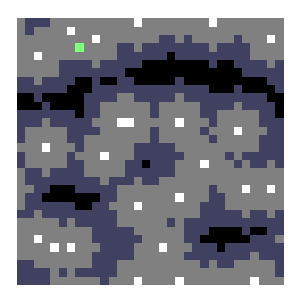
\includegraphics{00_000_grid.eps}
}
\caption["`Leeres Szenario"' ohne Hindernisse]{"`Leeres Szenario"' ohne Hindernisse}
\label{empty_grid:fig}
\end{figure}

\subsection{Szenario mit zuf�llig verteilten Hindernissen}\label{random_scenario_definition:sec}

Zwei Parameter bestimmen das Aussehen des Szenarios mit zuf�llig verteilten Hindernissen, zum einen der Prozentsatz an Hindernissen an der Gesamtzahl der Felder des Torus (Hindernissanteil~\(\lambda_{h}\)), zum anderen der Grad inwieweit die Hindernisse zusammenh�ngen (Verkn�pfungsfaktor~\(\lambda_{p}\)).\\
Bei der Erstellung des Szenarios bestimmt \(\lambda_{p}\) die Wahrscheinlichkeit f�r jedes einzelne angrenzende freie Feld, dass beim Verteilen der Hindernisse nach dem Setzen eines Hindernisses dort sofort ein weiteres Hindernis gesetzt wird. \(\lambda_{p} = 0.0\) erg�be somit eine v�llig zuf�llig verteilte Menge an Hindernissen, w�hrend ein Wert von \(1.0\) eine oder mehrere stark zusammenh�ngende Strukturen schafft. Wird der Prozentsatz an Hindernissen \(\lambda_{h}\) auf \(0.0\) gesetzt, dann entspricht diesem dem oben erw�hnten leeren Szenario. Ein Wert von \(1.0\) w�rde eine v�llige Abdeckung des Torus bedeuten und w�re f�r einen Test somit unbrauchbar. Hier sollen nur geringe Werte bis \(0.4\) betrachtet werden, wobei sp�ter in Tests sich auf Werte bis \(0.2\) beschr�nkt wird, da bei gro�en Hindernissanteil die lokalen Entscheidungen einzelner Agenten zu wichtig werden, da das Zielobjekt sich oft nur in einem kleinen Bereich aufh�lt TODO

In Abbildung~(\ref{random_grid_005:fig}), Abbildung~(\ref{random_grid_01:fig}), Abbildung~(\ref{random_grid_02:fig}) und Abbildung~(\ref{random_grid_04:fig}) werden Beispiele f�r zuf�llige Szenarien gegeben mit \(\lambda_{h} = 0.05\), \(0.1\), \(0.2\) bzw. \(0.4\) und \(\lambda_{p} = 0.01\), \(0.5\) bzw. \(0.99\).

\begin{figure}[htbp]
\centerline{	
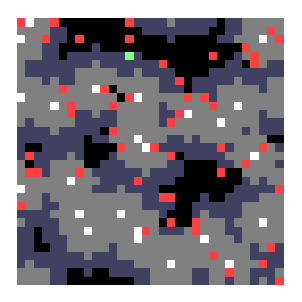
\includegraphics{005_001_grid.eps}
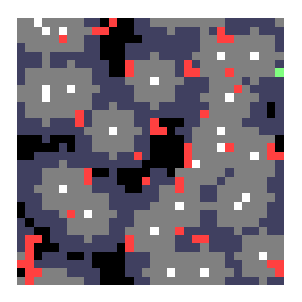
\includegraphics{005_050_grid.eps}
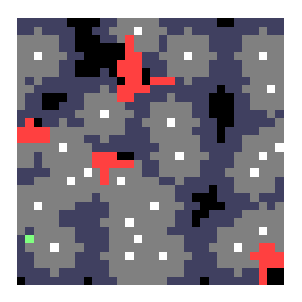
\includegraphics{005_099_grid.eps}
}
\caption[Szenario mit zuf�llig verteilten Hindernissen mit $\lambda_{h} = 0.05$] {Szenario mit zuf�llig verteilten Hindernissen mit Hindernissanteil \(\lambda_{h} = 0.05\) und Verkn�pfungsfaktor \(\lambda_{p} = 0.01\), \(0.5\) bzw. \(0.99\).}
\label{random_grid_005:fig}
\end{figure}

\begin{figure}[htbp]
\centerline{	
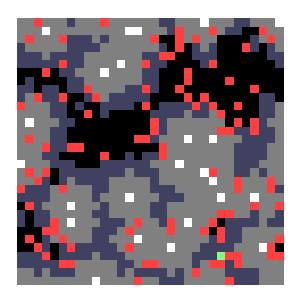
\includegraphics{01_001_grid.eps}
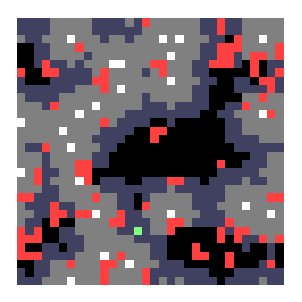
\includegraphics{01_050_grid.eps}
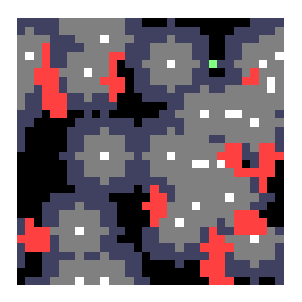
\includegraphics{01_099_grid.eps}
}
\caption[Szenario mit zuf�llig verteilten Hindernissen mit $\lambda_{h} = 0.1$] {Szenario mit zuf�llig verteilten Hindernissen mit Hindernissanteil \(\lambda_{h} = 0.1\) und Verkn�pfungsfaktor \(\lambda_{p} = 0.01\), \(0.5\) bzw. \(0.99\).}
\label{random_grid_01:fig}
\end{figure}

\begin{figure}[htbp]
\centerline{	
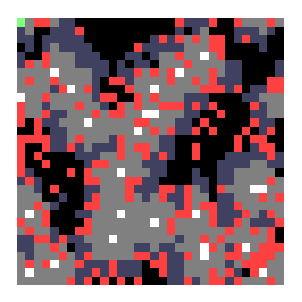
\includegraphics{02_001_grid.eps}
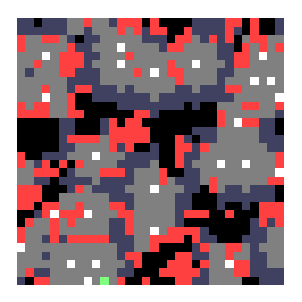
\includegraphics{02_050_grid.eps}
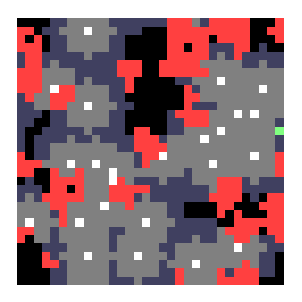
\includegraphics{02_099_grid.eps}
}
\caption[Szenario mit zuf�llig verteilten Hindernissen mit $\lambda_{h} = 0.2$] {Szenario mit zuf�llig verteilten Hindernissen mit Hindernissanteil \(\lambda_{h} = 0.2\) und Verkn�pfungsfaktor \(\lambda_{p} = 0.01\), \(0.5\) bzw. \(0.99\).}
\label{random_grid_02:fig}
\end{figure}

\begin{figure}[htbp]
\centerline{	
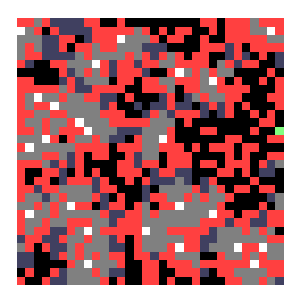
\includegraphics{04_001_grid.eps}
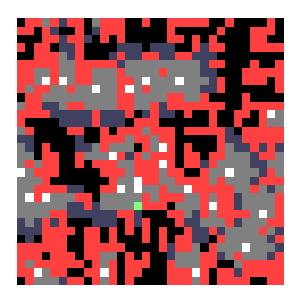
\includegraphics{04_050_grid.eps}
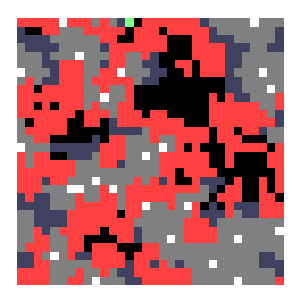
\includegraphics{04_099_grid.eps}
}
\caption[Szenario mit zuf�llig verteilten Hindernissen mit $\lambda_{h} = 0.4$] {Szenario mit zuf�llig verteilten Hindernissen mit Hindernissanteil \(\lambda_{h} = 0.4\) und Verkn�pfungsfaktor \(\lambda_{p} = 0.01\), \(0.5\) bzw. \(0.99\).}
\label{random_grid_04:fig}
\end{figure}


\subsection{S�ulen Szenario}

In diesem Szenario werden regelm��ig, mit jeweils 7 Feldern Zwischenraum zueinander,  Hindernisse auf dem Torus verteilt. Idee ist, dass die Agenten eine kleine Orientierungshilfe besitzen sollen, aber gleichzeitig m�glichst wenig Hindernisse verteilt werden. Das Zielobjekt startet an zuf�lliger Position, die Agenten starten mit m�glichst gro�em Abstand zum Zielobjekt. Abbildung~\ref{pillar_grid:fig} zeigt ein Beispiel f�r den Startzustand eines solchen Szenarios, bei der das Zielobjekt sich in der Mitte und die Agenten am Rand befinden.

\begin{figure}[htbp]
\centerline{	
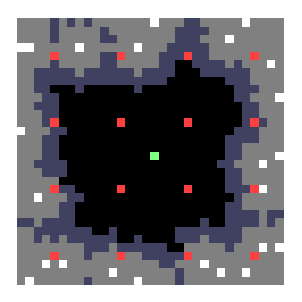
\includegraphics{pillar_grid.eps}
}
\caption[Startzustand des S�ulen Szenarios]{Startzustand des S�ulen Szenarios mit regelm��ig angeordneten Hindernissen und zuf�lliger Verteilung von Agenten mit m�glichst gro�em Abstand zum Zielobjekt}
\label{pillar_grid:fig}
\end{figure}



\subsection{Schwieriges Szenario}\label{difficult_scenario:sec}

Hier wird der Torus an der rechten Seite vollst�ndig durch Hindernisse blockiert, um den Torus zu halbieren. Alle Agenten starten (zuf�llig verteilt) am linken Rand, der Zielagent startet auf der rechten Seite.\\
In regelm��igen Abst�nden (7 Felder Zwischenraum) befindet sich eine vertikale Reihe von Hindernissen mit �ffnungen von 4 Feldern Breite abwechselnd im oberen Viertel und dem unteren Viertel.\\
Idee dieses Szenarios ist es, zu testen, inwieweit die Agenten durch die �ffnungen zum Ziel finden k�nnen. Ohne Orientierung an den �ffnungen und anderen Agenten ist es sehr schwierig, sich durch das Szenario zu bewegen. Die sp�ter besprochenen Tests in Kapitel~\ref{test_schwieriges_szenario:sec} werden zeigen, dass dieses Szenario besonders schwierig f�r sich zuf�llig bewegende Agenten und Agenten mit einfacher Heuristik ist. Sp�ter in Kapitel~\

Abbildung~\ref{difficult_grid:fig} zeigt die Startkonfiguration des Szenarios.

\begin{figure}[htbp]
\centerline{	

\includegraphics{difficult_grid.eps}
}
\caption[Schwieriges Szenario]{Schwieriges Szenario mit fester, wallartiger Verteilung von Hindernissen in regelm��igen Abst�nden und mit �ffnungen, mit den Agenten mit zuf�lligem Startpunkt am linken Rand und mit dem Zielobjekt mit festem Startpunkt rechts oben}
\label{difficult_grid:fig}
\end{figure}



\section{Bestimmung der Qualit�t eines Algorithmus}\label{qualitaet:sec}

Die Qualit�t eines Algorithmus zu einem Problem wird anhand des Anteils der Zeit berechnet, die er das Zielobjekt w�hrend des Problems �berwachen (d.h. das Zielobjekt innerhalb einer Distanz von h�chstens \emph{reward range} halten) konnte, relativ zur Gesamtzeit.\\
Die Qualit�t eines Algorithmus zu einer Anzahl von Problemen (also einem Experiment) wird Anhand des Gesamtanteil der Zeit berechnet, die er das Zielobjekt w�hrend aller Probleme �berwachen konnte, relativ zur Gesamtzeit aller Probleme.\\
Die Qualit�t eines Algorithmus entspricht dem Durchschnitt der Qualit�ten des Algorithmus mehrerer Experimente.\\
Die Halbzeitqualit�t eines Algorithmus zu einem Problem entspricht dem Anteil der Zeit, die der Algorithmus das Zielobjekt w�hrend jeweils der zweiten H�lfte des Problems �berwachen konnte, relativ zur halben Gesamtzeit.\\
Die Halbzeitqualit�t eines Algorithmus zu einer Anzahl von Problemen entspricht dem Anteil der Zeit, die der Algorithmus das Zielobjekt w�hrend jeweils der zweiten H�lfte des Problems �berwachen konnte, relativ zur halben Gesamtzeit aller Probleme.\\
Die Halbzeitqualit�t eines Algorithmus entspricht dem Durchschnitt aller Halbzeitqualit�ten des Algorithmus mehrerer Experimente.\\
Ein Vergleich der Qualit�t mit der Halbzeitqualit�t eines Algorithmus erm�glicht einen Einblick, wie gut sich der Algorithmus verh�lt, nachdem er sich auf das Problem bereits eine Zeit lang einstellen konnte.\\

\chapter{Agenten}

\section{Sensoren}\label{sensoren:sec}

Jeder Agent besitzt 3 Gruppen mit jeweils 8 Sensoren. Alle Sensoren sind visuelle, bin�re Sensoren mit begrenzter Reichweite und k�nnen nur feststellen, ob sich in ihrem Sichtbereich ein entsprechendes Objekt befindet oder nicht. Andere Objekte blockieren die Sicht, Sichtlinien werden durch einen einfachen Bresenham-Algorithmus bestimmt.\\
Jede Gruppe von Sensoren nimmt einen anderen Typ von Objekt wahr. Die erste Gruppe nimmt das Zielobjekt, die zweite Gruppe andere Agenten und die dritte Gruppe Hindernisse wahr.\\
Sensoren sind jeweils bestimmte Richtungen ausgerichtet (Norden, Osten, S�den und Westen, wobei auf den Abbildungen in dieser Arbeit Norden immer oben ist) und wird auf ``wahr'' (\(1\)) gesetzt, wenn sich in dem Sichtbereich des Sensors ein entsprechendes Objekt befindet.\\
Die 8 Sensoren in einer Gruppe sind in 4 Richtungen mit jeweils einem Sensorenpaar aufgeteilt. Ein Sensorenpaar besteht aus zwei Sensoren mit unterschiedlich gro�er Sichtweite, mit der der Agent also rudiment�r die Entfernung zu anderen Objekten feststellen kann. 

\[
\underbrace{z_{s_{N}} z_{r_{N}} z_{s_{O}} z_{r_{O}} z_{s_{S}} z_{r_{S}} z_{s_{W}} z_{r_{W}}}_{Erste~Gruppe~(Zielobjekt)}
\underbrace{a_{s_{N}} a_{r_{N}} a_{s_{O}} a_{r_{O}} a_{s_{S}} a_{r_{S}} a_{s_{W}} a_{r_{W}}}_{Zweite~Gruppe~(Agenten)}
\underbrace{h_{s_{N}} h_{r_{N}} h_{s_{O}} h_{r_{O}} h_{s_{S}} h_{r_{S}} h_{s_{W}} h_{r_{W}}}_{Dritte~Gruppe~(Hindernisse)}
\]

TODO darauf Bezug nehmen

\begin{verbatim}
TODO Beispiele f�r Sensoren
a) 10 00 00 00 . 00 00 00 00 . 00 00 00 00
b) 00 00 00 00 . 00 00 00 00 . 00 00 00 00
c) 00 00 00 00 . 11 00 10 00 . 00 00 00 00
d) 00 00 00 00 . 00 00 00 00 . 00 00 00 00
e) 00 00 00 00 . 00 00 00 00 . 00 00 00 00
\end{verbatim}



Die Sichtweite des ersten Sensors eines Paares wird �ber den Parameter \emph{sight range} bestimmt, die Sichtweite des zweiten Sensors �ber den Parameter \emph{reward range} (siehe auch Kapitel~\ref{sichtbarket:sec}). Allgemein soll \emph{sight range = 5.0} und \emph{reward range = 2.0} betragen, der �berwachte Bereich ist also eine Teilmenge des sichtbaren Bereichs. Anzumerken sei hier, dass deshalb ein Sensorenpaar (0\/1) nicht auftreten kann.\\
Sei \(r(O1, O2)\) die Distanz zwischen dem Objekt, das die Sensordaten erfasst und dem n�chstliegenden Objekt des Typs, den der Sensor wahrnehmen kann, dann gibt es folgende F�lle:

\begin{enumerate}
\item (0/0) : \(r(O_1, O_2) > \) \emph{sight range} (kein passendes Objekt in Sichtweite)
\item (1/0) : \emph{reward range} \( < r(O_1, O_2) \le \) \emph{sight range} (Objekt in Sichtweite)
\item (1/1) : \(r(O_1, O_2) \le \) \emph{reward range} (Objekt in Sicht- und �berwachungsreichweite)
\item (0/1) : \emph{reward range} \(\ge r(O_1, O_2) > \) \emph{sight range} (Fall kann nicht auftreten, da \emph{reward range} \( < \) \emph{sight range})
\end{enumerate}

In Abbildung ~\ref{sight_directions:fig} sind alle Sichtkegel (dunkler und heller Bereich) und �berwachungsreichweiten (heller Bereich) f�r die einzelnen Richtungen dargestellt. 

TODO von 3-5 auf 2-5 um�ndern

\begin{figure}[htbp]
\centerline{	
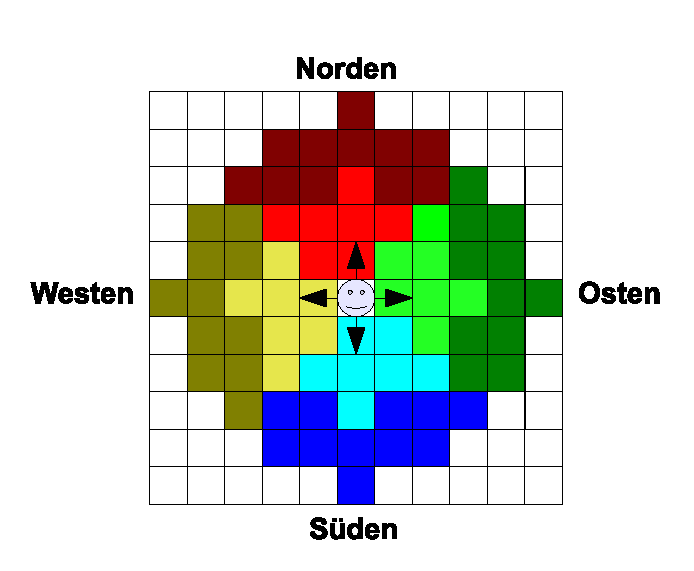
\includegraphics{sight_directions.eps}
}
\caption[Sicht- und �berwachungsreichweite eines Agenten]{Sicht- (2.0) und �berwachungsreichweite (5.0) eines Agenten, jeweils f�r die einzelnen Richtungen}
\label{sight_directions:fig}
\end{figure}

\section{F�higkeiten}\label{agent_abilities:sec}

Jeder Agent kann in jedem Schritt zwischen vier verschiedenen Aktionen w�hlen, die den vier Richtungen (Norden, Osten, S�den, Westen), bei der der Agent sich nicht bewegt, entsprechen. Agenten k�nnen pro Zeiteinheit genau einen Schritt durchf�hren. Das Zielobjekt kann je nach Szenarioparameter mehrere Schritte ausf�hren.

\section{Ablauf der Bewegung}
Alle Agenten werden nacheinander in der Art abgearbeitet, dass der jeweilige Agent die aktuellen Sensordaten aus der Umgebung holt und anhand dieser die n�chste Aktion bestimmt. Ung�ltige Aktionen, d.h. der Versuch sich auf ein besetztes Feld zu bewegen, schlagen fehl und der Agent f�hrt in diesem Schritt keine Aktion aus, wird aber nicht weiter bestraft. Eine detaillierte Beschreibung der Bewegung im Kontext anderer Agenten und Programmteile wird in Kapitel~\ref{reihenfolge:sec} gegeben.

\section{Grunds�tzliche Algorithmen der Agenten}

Neben denjenigen Algorithmen, die auf LCS basieren und in Kapitel~\ref{lcs:cha} besprochen werden, gibt es folgende Grundtypen, die dazu dienen, die Qualit�t der anderen Algorithmen einzuordnen. Wesentliches Merkmal im Vergleich zu auf LCS basierenden Algorithmen ist, dass sie statische, handgeschriebene Regeln benutzen und den Erfolg oder Misserfolg ihrer Aktionen ignorieren, d.h. ihre Regeln nicht anpassen.

\subsection{``Zuf�lliger Algorithmus''}\label{randomized_movement:sec}
Bei diesem Algorithmus wird in jedem Schritt wird eine zuf�llige Aktion ausgef�hrt. Abbildung ~(\ref{agent_random:fig}) zeigt eine Beispielsituation bei der der Agent jegliche Sensordaten ignoriert und eine Aktion zuf�llig ausw�hlen wird.

\begin{figure}[htbp]
\centerline{	
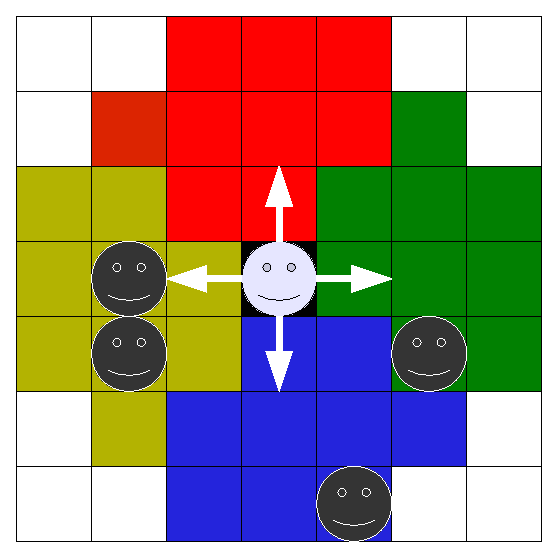
\includegraphics{agent_random.eps}
}
\caption[Sich zuf�llig bewegender Agent]{Agent bewegt sich in eine zuf�llige Richtung (oder bleibt stehen)}
\label{agent_random:fig}
\end{figure}

\subsection{Einfache Heuristik}\label{simple_heuristik:sec}
Ist das Zielobjekt in Sichtweite, bewegt sich ein Agent mit dieser Heuristik  auf das Zielobjekt zu, ist es nicht in Sichtweite, f�hrt er eine zuf�llige Aktion aus. Abbildung ~(\ref{simple_agent_to_goal:fig}) zeigt eine Beispielsituation bei der sich das Zielobjekt (Stern) im S�den befindet, der Agent mit einfacher Heuristik die anderen Agenten ignoriert und sich auf das Ziel zubewegen m�chte. 

\begin{figure}[htbp]
\centerline{	
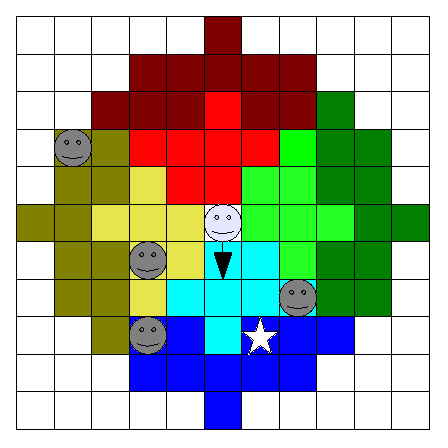
\includegraphics{simple_agent_to_goal.eps}
}
\caption[Agent mit einfacher Heuristik]{Agent mit einfacher Heuristik: Sofern es sichtbar ist bewegt sich der Agent auf das Zielobjekt zu.}
\label{simple_agent_to_goal:fig}
\end{figure}

\subsection{Intelligente Heuristik}\label{intelligent_heuristik:sec}
Ist der Zielobjekt in Sicht, verh�lt sich diese Heuristik wie die einfache Heuristik. Ist das Zielobjekt dagegen nicht in Sicht, wird versucht, anderen Agenten auszuweichen, um ein m�glichst breit gestreutes Netz aus Agenten aufzubauen. In der Implementation hei�t das, dass unter allen Richtungen, in denen kein anderer Agent gesichtet wurde, eine Richtung zuf�llig ausgew�hlt wird und falls alle Richtungen belegt (oder alle frei) sind, wird aus allen Richtungen eine zuf�llig ausgew�hlt wird. In Abbildung~(\ref{intelligent_agent:fig}) sieht der Agent das Zielobjekt nicht und w�hlt deswegen eine Richtung, in der die Sensoren keine Agenten anzeigt, in diesem Fall Norden.

\begin{figure}[htbp]
\centerline{	
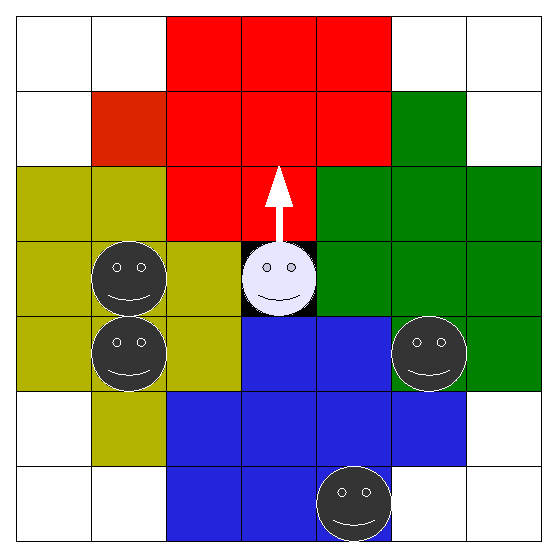
\includegraphics{intelligent_agent.eps}
}
\caption[Agent mit intelligenter Heuristik]{Agent mit intelligenter Heuristik: Falls das Zielobjekt nicht sichtbar ist bewegt sich der Agent von anderen Agenten weg.}
\label{intelligent_agent:fig}
\end{figure}

\chapter{Das Zielobjekt}


Die Typen von Zielobjekten werden zum einen �ber ihre Geschwindigkeit und zum anderen �ber ihre Bewegungsart definiert. Neben der Gr��e des Torus und den Hindernissen tr�gt der Typ des Zielobjekts wesentlich zur Schwierigkeit eines Szenarios bei, da dieser die Aufenthaltswahrscheinlichkeiten des Zielobjekts unter Einbeziehung des Zustands des letzten Zeitschritts bestimmt. Die Schwierigkeit bestimmt sich �ber die Summe der erwarteten Aufenthaltswahrscheinlichkeiten in nicht �berwachten Feldern geteilt durch die Summe der Aufenthaltswahrscheinlichkeiten in �berwachten Feldern.

\section{Basiseigenschaften}

Im wesentlichen entspricht ein Zielobjekt einem Agenten, d.h. das Zielobjekt kann sich bewegen und besitzt Sensoren. 

Gemeinsam haben alle Arten von Bewegungen des Zielobjekts, dass, wenn dem Algorithmus kein freies Feld zur Verf�gung steht, ein zuf�lliges, freies Feld in der N�he ausgew�hlt und dort hingesprungen wird. Dies kommt einem Neustart gleich und ist notwendig um eine Verf�lschung des Ergebnisses zu verhindern, das daher r�hren kann, dass ein oder mehrere Agenten (zusammen mit eventuellen Hindernissen) alle vier Bewegungsrichtungen des Zielobjekts blockieren.\\
Andererseits ist auch der Sprung eine Verf�lschung, falls bei einem Durchlauf eine ganze Anzahl von Spr�ngen durchgef�hrt worden sein, sollte man deshalb das Ergebnis verwerfen und andere Random-Seed Werte benutzen.

TODO wie oft das aufgetreten ist

TODO benachbarte Hindernisse aus Bewegung ausschliessen, N�hesensor

\section{Typen von Zielobjekten}

\subsection{Typ ``Total Random''}
Ein Zielobjekt dieses Typs springt zu einem zuf�lligen (freien) Feld auf dem Torus. Mit dieser Einstellung kann die Abdeckung des Algorithmus gepr�ft werden, d.h. inwieweit die Agenten jeweils au�erhalb der �berwachungsreichweite anderer Agenten bleiben. Jegliche Anpassung an die Bewegung des Zielobjekts ist hier wenig hilfreich, ein Agent kann nicht einmal davon ausgehen, dass sich das Zielobjekt in der N�he seiner Position der letzten Zeiteinheit befindet. Die Aufenthaltswahrscheinlichkeit f�r jedes freie Feld ist hierbei \(\frac{1}{n}\), wobei \(n\) die Anzahl der freien Felder entspricht.

\subsection{``Random Movement''}
Wie ``Random Movement'' bei Agenten (~\ref{randomized_movement:sec}). Sind alle m�glichen Felder belegt, wird wie oben beschrieben auf ein zuf�lliges Feld gesprungen. Diesen Fall au�en vorgelassen betr�gt die Aufenthaltswahrscheinlichkeit f�r die 4 angrenzenden Felder jeweils \(\frac{1}{5}\) und das Zielobjekt bleibt mit Wahrscheinlichkeit \(\frac{1}{5}\) stehen.

\subsection{``One direction change''}
Mit dieser Einstellung wird die der letzten Richtung entgegengesetzten Richtung aus der Menge der Auswahlm�glichkeiten entfernt und von den verbleibenden drei Richtungen (plus der Aktion ``Stehenbleiben'') eine zuf�llig ausgew�hlt. Sind alle drei Richtungen versperrt, wird stehengeblieben.\\
War die letzte Aktion nicht eine Bewegungsrichtung, sondern die Aktion ``Stehenbleiben'', so wird eine zuf�llige Richtung ausgew�hlt. Sind alle Richtungen versperrt, wird auch hier wieder auf ein zuf�lliges Feld gesprungen.
Die Aufenthaltswahrscheinlichkeit betr�gt im Fall ohne angrenzende Hindernisse f�r die Felder vor, links und rechts (relativ zur Bewegungsrichtung im vergangenen Zeitschritt) also \(\frac{1}{3}\). In Abbildung~\ref{goal_agent_one_direction_change:fig} ist eine Beispielsituation zu sehen, bei der der Zielagent sich zuletzt nach Norden bewegt hat und nun zwischen Norden, Westen und Osten ausw�hlen kann.

\begin{figure}[htbp]
\centerline{	
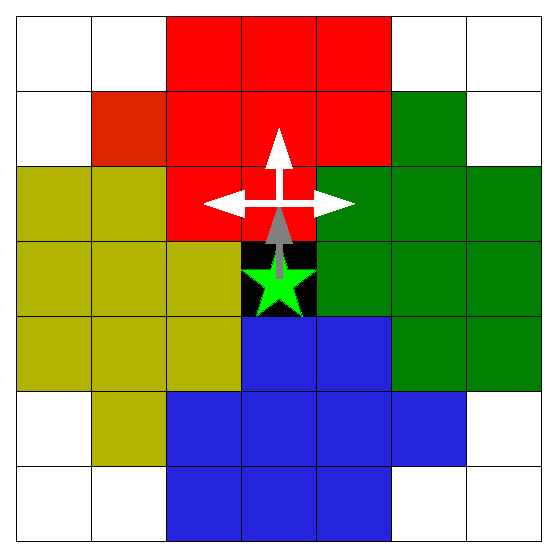
\includegraphics{goal_direction_change.eps}
}
\caption[Zielobjekt mit maximal einer Richtungs�nderung]{Zielobjekt macht pro Schritt maximal eine Richtungs�nderung}
\label{goal_agent_one_direction_change:fig}
\end{figure}

\subsection{``Always same direction''}
Der Zielobjekt versucht, immer Richtung Norden zu gehen. Ist das Zielfeld blockiert, w�hlt er ein zuf�lliges, angrenzendes, freies Feld im Westen oder Osten. Anzumerken ist, dass dies zus�tzliche F�higkeiten darstellen, d.h. das Zielobjekt kann feststellen, ob sich direkt angrenzend ein Hindernis im Norden befindet, w�hrend normale Agenten, was die Distanz betrifft, keine Informationen dar�ber besitzen k�nnen.\\
Sind auch die Felder im Westen und Osten belegt, springt er auf ein zuf�lliges freies Feld. Schafft es der Zielobjekt innerhalb von einer bestimmten Zahl (Breite des Spielfelds) von Schritten nicht, einen weiteren Schritt nach Norden zu gehen, wird ebenfalls gesprungen, um ein ``Festh�ngen'' an einem Hindernis zu vermeiden. Ohne Hindernisse ergibt sich also eine Aufenthaltswahscheinlichkeit von \(1.0\) im dar�berliegenden Feld im Norden. In Abbildung~\ref{goal_agent_always_same_direction:fig} sind drei Situationen dargestellt, zum einen ein wiederholtes hin- und herlaufen unter den Hindernissen, der Weg links um die Hindernisse herum und der Weg rechts um die Hindernisse herum.

TODO im Bild den Pfeil nach rechts bzw. links raus, wo er bereits im Norden frei ist

\begin{figure}[htbp]
\centerline{	
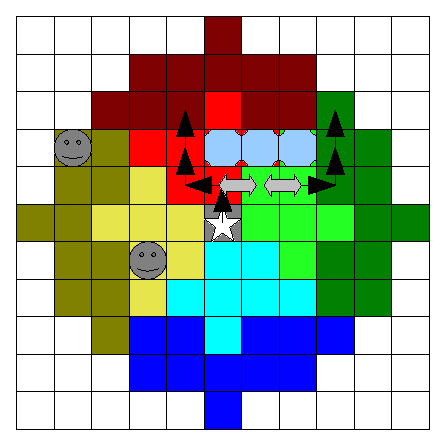
\includegraphics{goal_always_same_direction.eps}
}
\caption[Zielobjekt das sich, wenn m�glich, immer nach Norden bewegt]{Zielobjekt bewegt sich, wenn m�glich, immer nach Norden}
\label{goal_agent_always_same_direction:fig}
\end{figure}

\subsection{``Intelligent (Open)''}
Das Zielobjekt versucht bei der Auswahl der Aktion m�glichst die Aktion zu w�hlen, bei der es au�erhalb der Sichtweite der Agenten bleibt, es werden also alle Richtungen gestrichen, in denen ein anderer Agent gesichtet wird. Von den verbleibenden Richtungen werden au�erdem mit 20\% Wahrscheinlichkeit alle Richtungen gestrichen, in denen sich ein Hindernis befindet. Sind alle Richtungen gestrichen worden, bewegt sich das Zielobjekt zuf�llig. Sind alle Richtungen blockiert, springt es wie in den anderen Varianten auch auf ein zuf�lliges Feld. In Abbildung~\ref{goal_agent_intelligent_open:fig} wird die Richtung Westen gestrichen, da sich dort ein Agent befindet. Im Norden und Osten befinden sich Hindernisse, diese Richtungen werden jeweils mit 20\% gestrichen, w�hrend die Richtung S�den mit Sicherheit als Auswahlm�glichkeit �brig bleibt. Die Aufenthaltswahrscheinlichkeit f�r Norden und Osten w�ren also jeweils \(\frac{8*8}{3*10*10}+\frac{2*8}{2*10*10} = \frac{88}{300}\) und \(\frac{8*8}{3*10*10}+\frac{2*2*8}{2*10*10}+\frac{2*2}{10*10}=\frac{124}{300}\) f�r den S�den.

\begin{figure}[htbp]
\centerline{	
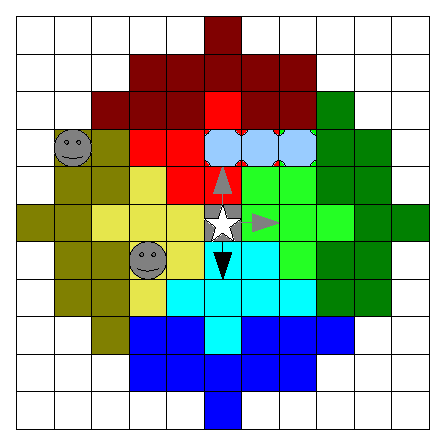
\includegraphics{goal_intelligent_open.eps}
}
\caption[Sich intelligent verhaltendes Zielobjekt der Agenten und Hindernissen ausweicht]{Zielobjekt bewegt sich mit bestimmter Wahrscheinlichkeit von Agenten und gr��erer Wahrscheinlichkeit von Hindernissen weg}
\label{goal_agent_intelligent_open:fig}
\end{figure}

\subsection{``Intelligent (Hide)''}
Das Zielobjekt vermeidet Agenten wie bei ``Intelligent (Open)'', streicht aber statt Richtungen mit Hindernissen Richtungen ohne Hindernisse mit 20\% Wahrscheinlichkeit, tendiert also eher dazu, auf Hindernisse zuzugehen. Idee ist, dass es sich dadurch m�glicherweise den Blicken der Agenten entziehen kann. Betrachten wir in Abbildung~\ref{goal_agent_intelligent_hide:fig} die selbe Situation wie bei ``Intelligent (Open)'' so sind die Aufenthaltswahrscheinlichkeiten von Norden und Osten mit denen von S�den vertauscht.

\begin{figure}[htbp]
\centerline{	
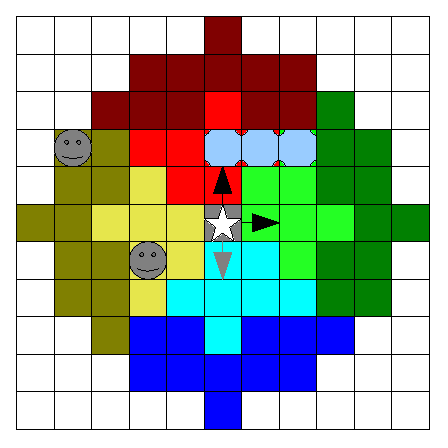
\includegraphics{goal_intelligent_hide.eps}
}
\caption[Sich intelligent verhaltendes Zielobjekt der Agenten ausweicht und Hindernisse sucht]{Zielobjekt bewegt sich von Agenten weg und mit bestimmter Wahrscheinlichkeit auf Hindernisse zu}
\label{goal_agent_intelligent_hide:fig}
\end{figure}

\subsection{``LCS''}
Eine LCS Implementierung, die der Implementierung eines LCS Agenten entspricht. Das Ziel des Zielobjekts ist es hier aber, es zu vermeiden, Agenten zu �berwachen (bzw. umgekehrt eine �berwachung durch andere Agenten zu vermeiden). Eine genaue Beschreibung folgt im Kapitel~\ref{lcs:cha} und soll hier nur der Vollst�ndigkeit halber erw�hnt werden.

TODO auch ein eigenes goal agent lcs kapitel machen
TODO Pendelbewegung?
TODO Fester Pfad?

\chapter{Ablauf der Simulation}\

\section{Hauptschleife}

In der Hauptschleife (siehe Programm~\ref{mainExperiment:pro}) wird ein Experiment mit vorgegebener Konfiguration (``\emph{Configuration}'') durchgef�hrt. Dabei werden eine Anzahl von Problemen abgearbeitet, bei denen jeweils der Torus auf den Startzustand gesetzt, das eigentliche Problem berechnet und ein neuer \emph{random seed} Wert gesetzt wird.


\newlisting{Zentrale Schleife f�r einzelne Experimente}{mainExperiment:pro}
/**
 * F�hrt eine Anzahl von Problemen aus
 * @param experiment_nr Nummer des auszuf�hrenden Experiments
 */
  public void doOneMultiStepExperiment(int experiment_nr) {
    int currentTimestep = 0;

  /**
   * number of problems for the same population
   */
    for (int i = 0; i < Configuration.getNumberOfProblems(); i++) {

    /**
     * Erstellt einen neuen Torus und verteilt Agenten und das Zielobjekt neu
     */
      BaseAgent.grid.resetState();

    /**
     * F�hre Problem aus und aktualisiere aktuellen Zeitschritt
     */
      currentTimestep = doOneMultiStepProblem(currentTimestep);

    /**
     * Initialisiere neuen "Random Seed" Wert
     */
      Misc.initSeed(Configuration.getRandomSeed() + 
        experiment_nr * Configuration.getNumberOfProblems() + 1 + i);
    }
  }
\end{lstlisting}


\section{Reihenfolge der Ausf�hrung (\emph{doOneMultiStepProblem()})}\label{reihenfolge:sec}

TODO vielleicht erst noch eine allgemeine �bersicht geben

F�r die Berechnung eines einzelnen Problems (``\emph{doOneMultiStepProblem()}'') stellt sich die Frage nach der Genauigkeit und der Reihenfolge der Abarbeitung, da die Simulation nicht parallel, sondern schrittweise auf einem diskreten Torus abl�uft. Dies kann u.U. dazu f�hren, dass je nach Position in der Liste abzuarbeitender Agenten die Informationen �ber die Umgebung unterschiedlich alt sind. Die Frage ist deshalb, in welcher Reihenfolge Sensordaten ermittelt, ausgewertet, Agenten bewegt, intern sich selbst bewertet und global die Qualit�t gemessen wird.\\
Da eine Aktion auf Basis der Sensordaten ausgew�hlt wird, ist die erste Restriktion, dass eine Aktion nach der Verarbeitung der Sensordaten stattfinden muss. Und da Aktionen bewertet werden sollen, also jeweils der Zustand nach der Bewegung mit dem gew�nschten Zustand verglichen werden soll, ist die zweite Restriktion, dass die Bewertung einer Aktion nach dessen Ausf�hrung stattfinden muss.\\
Ansonsten ergeben sich folgende M�glichkeiten:

\begin{enumerate}
\item F�r alle Agenten werden erst einmal die neuen Sensordaten erfasst und sich f�r eine Aktion entschieden. Sind alle Agenten abgearbeitet, werden die Aktionen ausgef�hrt.
\item Die Agenten werden nacheinander abgearbeitet, es werden jeweils neue Sensordaten erfasst und sich sofort f�r eine neue Aktion entschieden. 
\end{enumerate}

Bei der ersten M�glichkeit haben alle Agenten die Sensordaten vom Beginn der Zeiteinheit, w�hrend bei der zweiten M�glichkeit sp�ter verarbeitete Agenten bereits die Aktionen der bereits berechneten Agenten miteinbeziehen k�nnen. Umgekehrt k�nnen dann fr�here Agenten bessere Positionen fr�her besetzen. Da aufgrund der primitiven Sensoren nicht davon auszugehen ist, dass Agenten beginnende Bewegungen (und somit deren jeweilige Zielposition) anderer Agenten einbeziehen k�nnen, soll jeder Agent von den Sensorinformationen zu Beginn der Zeiteinheit ausgehen.\\
Wenn sich mehrere Agenten auf dasselbe Feld bewegen wollen, dann spielt die Reihenfolge der Ausf�hrung der Aktionen eine Rolle. Wird die Liste der Agenten einfach linear abgearbeitet, k�nnen Agenten mit niedriger Position in der Liste die Aktion auf Basis j�ngerer Sensordaten f�llen. Dies kann dazu f�hren, dass Aktionen von Agenten mit h�herer Position in der Liste eher fehlschlagen, da das als frei angenommene Feld nun bereits besetzt ist. Da es keinen Grund gibt, Agenten mit niedrigerer Position zu bevorteilen, werden die Aktionen der Agenten in zuf�lliger Reihenfolge abgearbeitet.\\
Bez�glich der Bewegung ergibt sich hierbei eine weitere Frage, n�mlich wie unterschiedliche Bewegungsgeschwindigkeiten behandelt werden sollen, da alle Agenten eine Einheitsgeschwindigkeit von maximal einem Feld pro Zeiteinheit haben, w�hrend sich das Zielobjekt je nach Szenario gleich eine ganze Anzahl von Feldern bewegen kann (siehe auch Kapitel~\ref{base_properties_goal:sec}).
Die Entscheidung fiel hier auf eine zuf�llige Verteilung. Kann sich das Zielobjekt um \(n\) Schritte bewegen, so wird seine Bewegung in \(n\) Einzelschritte unterteilt, die nacheinander mit zuf�lligen Abst�nden (d.h. Bewegungen anderer Agenten) ausgef�hrt werden.\\
Eine weitere Frage ist, wie das Zielobjekt diese weiteren Schritte festlegen soll. Hier soll ein Sonderfall eingef�hrt werden, sodass das Zielobjekt in einer Zeiteinheit mehrmals (\(n\)-mal) neue Sensordaten erfassen und sich f�r eine neue Aktion entscheiden kann.

\section{Messung der Qualit�t}\label{qualitaetsmessung:sec}

Eine konkrete Antwort kann man auf diese zwei Fragen nicht geben, sie h�ngt  davon ab, was man denn nun eigentlich erreichen m�chte, also auf welche Weise die Qualit�t des Algorithmus bewertet wird. Der naheliegendste Messzeitpunkt ist, nachdem sich alle Agenten bewegt haben. Da die Agenten und das Zielobjekt in einem Durchlauf gemeinsam nacheinander bewegt werden, stellt sich die Frage nicht, ob wom�glich vor der Bewegung des Zielobjekts die Qualit�t gemessen werden sollen. Eine Messung nach der Bewegung des Zielobjekts w�rde diesem erlauben, sich vor jeder Messung optimal zu positionieren, was in einer geringeren Qualit�t f�r den Algorithmus resultiert, da sich das Zielobjekt aus der �berwachungsreichweite anderer Agenten hinausbewegen kann. Letztlich ist es eine Frage der Problemstellung, denn eine Messung nach Bewegung des Zielobjekts bedeutet letztlich, dass ein Agent einen gerade aus seiner �berwachungsreichweite heraus laufenden Zielobjekts in diesem Schritt nicht mehr �berwachen kann.\\
Da ein wesentlicher Bestandteil die Kooperation (und somit die Abdeckung des Torus anstatt dem Verfolgen des Zielobjekts) sein soll, soll ein Bewertungskriterium sein, inwieweit der Einfluss des Zielobjekts minimiert werden soll. Auch findet, wenn man vom realistischen Fall ausgeht, die Bewegung des Zielobjekts gleichzeitig mit allen anderen Agenten statt. Die Qualit�t wird somit nach der Bewegung des Zielobjekts gemessen. Die �berlegung unterstreicht auch nochmal, dass es besser ist, das Zielobjekt insgesamt wie einen normalen (aber sich mehrmals bewegenden) Agenten zu behandeln.\\

\section{Reihenfolge der Ermittlung des \emph{base reward}}

Keine der bisher vorgestellten Varianten machen Gebrauch von einem sogenannten \emph{base reward}, d.h.  TODO

Schlie�lich bleibt die Frage danach, wann gepr�ft werden soll, ob das Zielobjekt in �berwachungsreichweite ist, und wann sich somit ein \emph{reward} ergeben soll. Wesentliche Punkte hierbei sind, dass der Algorithmus sich anhand der Sensordaten selbst bewertet und pro Zeitschritt die Sensordaten nur einmal erhoben werden. Letzteres folgt aus der Auslegung von XCS, der in der Standardimplementation darauf ausgelegt ist, dass der Reward jeweils genau einer Aktion zugeordnet ist. Daraus ergibt sich auch, dass der Reward von bin�rer Natur ist ("`Zielobjekt in �berwachungsreichweite"' oder "`Zielobjekt nicht in �berwachungsreichweite"'), weshalb Zwischenzust�nde f�r den Reward, der sich aus der mehrfachen Bewegung des Zielobjekts ergeben k�nnte, ausgeschlossen werden soll (z.B. "`War zwei von drei Schritten in der �berwachungsreichweite"' \(\Rightarrow \frac{2}{3}\) Reward). Insbesondere w�rde dies eine mehrfache Erhebung der Sensordaten erfordern.\\

TODO Rewarderhebung f�r normale Agenten irrelevant, evtl teilen und in XCS Kapitel

F�r den Reward ergeben sich somit folgende M�glichkeiten:

\begin{enumerate}
\item Ermittlung der einzelnen \emph{reward} Werte jeweils direkt nach der Ausf�hrung einer einzelnen Aktion
\item Ermittlung aller \emph{reward} Werte nach Ausf�hrung aller Aktionen der Agenten und des Zielobjekts
\end{enumerate}

Werden die \emph{reward} Werte sofort ermittelt (Punkt 1), dann bezieht sich der Wert auf die veralteten Sensordaten vor der Aktion, die Aktion selbst w�rde bei der Ermittlung des \emph{reward} Werts also ignoriert werden. Bei Punkt 2 m�sste man bis zum neuen Zeitschritt warten, bis neue Sensordaten ermittelt wurden.


\section{Zusammenfassung}
Zusammenfassend sieht der Ablauf aller Agenten (inklusive des Zielobjekts) also wie folgt aus:

\begin{figure}[H]
\setbox0\vbox{\small
\begin{enumerate}
\item Bestimmen der aktuellen \textbf{Qualit�t}
\item Erfassung aller \textbf{Sensordaten}
\item Bestimmung der jeweiligen {\bfseries {\em reward} Werte} f�r die einzelnen Objekte f�r den letzten Schritt
\item \textbf{Wahl der Aktion} anhand der Regeln des jeweiligen Agenten
\item \textbf{Ausf�hrung der Aktion} (in zuf�lliger Reihenfolge, das Zielobjekt wiederholt Schritte 1 und 2 nach der Ausf�hrung der Aktion)
\end{enumerate}
}
\centerline{\fbox{\box0}}
\end{figure}

\section{Implementierung eines Problemablaufs}\label{implementierung_ablauf:sec}

In der Schleife der Funktion zur Berechnung eines Experiments (Programm~\ref{mainExperiment:pro}) wird die Funktion zur Berechnung des Problems (\emph{doOneMultiStepProblem()} in Programm~\ref{mainProblem:pro}) aufgerufen. Dort wird, in einer weiteren Schleife �ber die Anzahl der maximalen Schritte, die Sicht aktualisiert (\emph{updateSight()}), die Qualit�t bestimmt (\emph{updateStatistics()}), die neuen Sensordaten und die n�chste Aktion ermittelt (\emph{calculateAgents()}, siehe Programm~\ref{mainCalculate:pro}), der \emph{reward} Wert ermittelt (\emph{rewardAgents()}, siehe Programm~\ref{mainReward:pro}) und schlie�lich die Objekte bewegt (\emph{moveAgents()}, siehe Programm~\ref{mainMove:pro}). Die konkrete Umsetzung der dort aufgerufenen Funktionen (insbesondere \emph{calculateNextMove()} und \emph{calculateReward()}) wird im Kapitel~\ref{lcs_variants:cha} erl�utert (bzw. in Kapitel~\ref{agents:cha} was die Heuristiken betrifft, wobei \emph{calculateReward()} dort keine Rolle spielt und eine leere Funktion aufgerufen wird).


\newlisting{Zentrale Schleife f�r einzelne Probleme}{mainProblem:pro}
/**
 * F�hrt eine Anzahl von Schritten auf dem aktuellen Torus aus
 * @param stepCounter Aktuelle Zeitschritt
 * @return Der Zeitschritt nach der Ausf�hrung
 */
  private int doOneMultiStepProblem(int stepCounter) {
  /**
   * Zeitpunkt bis zu dem das Problem ausgef�hrt wird
   */
    int steps_next_problem = 
      Configuration.getNumberOfSteps() + stepCounter;    
    for (int currentTimestep = stepCounter; 
         currentTimestep < steps_next_problem; currentTimestep++) {

    /**
     * Ermittle die Sichtbarkeit und erhebe Statistiken
     */
      BaseAgent.grid.updateSight();
      BaseAgent.grid.updateStatistics(currentTimestep);

    /**
     * Ermittle neue Sensordaten und berechne Aktionen der Agenten
     */
      calculateAgents(currentTimestep);

    /**
     * Ermittle den Reward f�r alle Agenten (nach dem ersten Schritt)
     */
      if(currentTimestep > stepCounter) {
        rewardAgents(currentTimestep);
      }

    /**
     * F�hre zuvor berechnete Aktionen aus
     */
      moveAgents();
    }

    /**
     * Abschlie�ende Ermittlung des Rewards
     */
    BaseAgent.grid.updateSight();
    rewardAgents(steps_next_problem);
    return steps_next_problem;
  }
\end{lstlisting}



\newlisting{Zentrale Bearbeitung (Sensordaten und Berechnung der neuen Aktion) aller Agenten und des Zielobjekts innerhalb eines Problems}{mainCalculate:pro}
/**
 * Berechnet die Aktionen und f�hrt sie in zuf�lliger Reihenfolge aus
 * @param gaTimestep der aktuelle Zeitschritt
 */
  private void calculateAgents(final long gaTimestep) {

  /**
   * Ermittle Sensordaten und bestimme n�chste Bewegung
   */
    for(BaseAgent a : agentList) {
      a.aquireNewSensorData();
      a.calculateNextMove(gaTimestep);
    }
    BaseAgent.goalAgent.aquireNewSensorData();
    BaseAgent.goalAgent.calculateNextMove(gaTimestep);
  }
\end{lstlisting}



\newlisting{Zentrale Bearbeitung (Verteilung des Rewards) aller Agenten und des Zielobjekts innerhalb eines Problems}{mainReward:pro}
/**
 * Verteilt den Reward an alle Agenten
 */
  private void rewardAgents(final long gaTimestep) {
    for(BaseAgent a : agentList) {
      a.calculateReward(gaTimestep);
    }
    BaseAgent.goalAgent.calculateReward(gaTimestep);
  }
\end{lstlisting}



\newlisting{Zentrale Bearbeitung (Ausf�hrung der Bewegung) aller Agenten und des Zielobjekts innerhalb eines Problems}{mainMove:pro}
/**
 * F�hrt die berechnete Bewegungen der Agenten in zuf�lliger Reihenfolge aus
 */
  private void moveAgents(long gaTimestep) {
  /**
   * Erstelle Ausf�hrungsliste f�r alle Objekte (Zielobjekt mehrfach)
   */
    int goal_speed = Configuration.getGoalAgentMovementSpeed();
    ArrayList<BaseAgent> random_list = 
      new ArrayList<BaseAgent>(agentList.size() + goal_speed);

    random_list.addAll(agentList);
    for(int i = 0; i < goal_speed; i++) {
      random_list.add(BaseAgent.goalAgent);
    }

  /**
   * F�hre die ermittelten Aktionen in zuf�lliger Reihenfolge aus
   *   (Zielobjekt kann mehrfach ausgef�hrt werden).
   */
    int[] array = Misc.getRandomArray(random_list.size());
    for(int i = 0; i < array.length; i++) {
      BaseAgent a = random_list.get(array[i]);
      a.doNextMove();
      if(a.isGoalAgent() && goal_speed > 1) {
        goal_speed--;
        a.aquireNewSensorData();
        a.calculateNextMove(gaTimestep);
        a.calculateReward(gaTimestep);
      }
    }
  }
\end{lstlisting}

\chapter{Szenario}

Im Wesentlichen sollen die hier besprochenen Algorithmen in einem \"Uberwachungsszenario getestet werden, d.h. die Qualit\"at eines Algorithmus wird anhand des Anteils der Zeit bewertet, die er das Zielobjekt \"uberwachen konnte, relativ zur Gesamtzeit. 

Verwendetes Umfeld wird ein quadratischer Torus sein, der aus quadratischen Feldern besteht.
Jedes bewegliche Objekt auf einem Feld kann sich nur auf eines der vier Nachbarfelder bewegen oder stehenbleiben. 
Die Felder k\"onnen entweder leer oder durch ein Objekt besetzt sein. Besetzte Felder k\"onnen nicht betreten werden. Es gibt drei verschiedene Arten von Objekten, unbewegliche Hindernisse, ein zu \"uberwachende Zielagent und Agenten. Zielagent und Agent bewegen sich anhand eines bestimmten Algorithmus anhand bestimmter Sensordaten.

TODO Aufl\"osen

\section{Problem-Instanzen}

Eine einzelne Probleminstanz entspricht einem Torus mit einer (abh\"angig vom verwendeten Random-Seed-Wert) bestimmten Anfangsbelegung mit bestimmten Objekten und bestimmten Parametern zur Sichtbarkeit. Die Parameter bestimmen, ob und wie Objekte andere Objekte die Sicht versperren und bis zu welcher Distanz der Zielagent von einem Agenten als �\"uberwacht� gilt, sofern die Sicht durch andere Objekte nicht versperrt ist.

Ein Experiment entspricht dem Test einer Anzahl von Probleminstanzen mit einer Reihe von Random-Seed-Werten.
In einem Durchlauf werden mehrere Experimente (jeweils mit unterschiedlichen Random-Seed-Wert-Reihen) durchgef\"uhrt.

\section{Qualit"at}

Problem-Qualit\"at eines Algorithmus zu einem Problem wird anhand des Anteils der Zeit berechnet, die er das Zielobjekt w\"ahrend des Problems \"uberwachen konnte, relativ zur Gesamtzeit. 
Experiment-Qualit\"at eines Algorithmus zu einer Anzahl von Problemen (einem Experiment) wird Anhand des Gesamtanteilder Zeit berechnet, die er das Zielobjekt w\"ahrend aller Probleme \"uberwachen konnte, relativ zur Gesamtzeit aller Probleme.
Qualit\"at eines Algorithmus entspricht dem Durchschnitt aller Experimentqualit\"aten des Algorithmus.

Halbzeit-Problem-Qualit\"at eines Algorithmus zu einem Problem entspricht dem Anteil der Zeit, die der Algorithmus das Zielobjekt w\"ahrend jeweils der zweiten H\"alfte des Problems \"uberwachen konnte, relativ zur halben Gesamtzeit.
Halbzeit-Experiment-Qualit\"at eines Algorithmus zu einer Anzahl von Problemen entspricht dem Anteil der Zeit, die der Algorithmus das Zielobjekt w\"ahrend jeweils der zweiten H\"alfte des Problems \"uberwachen konnte, relativ zur halben Gesamtzeit aller Probleme.
Die Halbzeitqualit\"at eines Algorithmus entspricht dem Durchschnitt aller Halbzeit-Experiment-Qualit\"aten eines Algorithmus.







\chapter{Agenten}

\section{Sensoren}

Jeder Agent besitzt 3 Gruppen mit jeweils 4 Bin\"arsensoren. Alle Sensoren sind visuelle Sensoren mit begrenzter Reichweite. Je nach Parameter des Szenarios wird die Sicht durch andere Objekten blockiert. Sichtlinien werden durch einen einfachen Bresenham-Linienalgorithmus bestimmt.
Jede Gruppe von Sensoren nimmt einen anderen Typ von Objekt wahr. Die erste Gruppe nimmt den Zielagenten, die zweite andere Agenten und die dritte Hindernisse.
Ein Sensor ist jeweils in eine bestimmte Richtung ausgerichtet (Norden, Osten, S\"uden, Westen) und wird auf ``wahr'' gesetzt, wenn sich in dem von der Sichtweite bestimmten Kegel ein entsprechendes Objekt befindet.

\section{F\"ahigkeiten}

Jeder Agent kann in jedem Schritt zwischen 5 verschiedenen Aktionen w\"ahlen, die den vier Richtungen plus einer Aktion, bei der der Agent sich nicht bewegt, entsprechen. Agenten k\"onnen pro Zeiteinheit genau einen Schritt durchf\"uhren. Der Zielagent kann je nach Szenario mehrere Schritte ausf\"uhren.
K\"onnte der Zielagent ebenfalls nur einen Schritt ausf\"uhren, w\"are das Problem sehr simpel, da der Zielagent Schwierigkeiten h\"atte, Agenten abzusch\"utteln, deren einzige Strategie es ist, sich in Richtung des Zielagenten zu bewegen.

\section{Ablauf der Bewegung}
Alle Agenten werden nacheinander in der Art abgearbeitet, dass der jeweilige Agent die aktuellen Sensordaten aus der Umgebung holt und anhand dieser die n\"achste Aktion bestimmt. Ung\"ultige Aktionen, d.h. der Versuch sich auf ein besetztes Feld zu bewegen, schlagen fehl und der Agent f\"uhrt in diesem Schritt keine Aktion aus, wird aber nicht weiter bestraft. Eine detaillierte Beschreibung wird in Kapitel~\ref{conclusion:cha} geliefert.

\section{Grunds\"atzliche Algorithmen der Agenten}

Neben denjenigen Algorithmen die auf LCS basieren und weiter untern besprochen werden, gibt es folgende Grundtypen, die dazu dienen, die Qualit\"at der anderen Algorithmen einzuordnen. Wesentliches Merkmal im Vergleich zu auf LCS basierenden Algorithmen ist, dass sie statische Regeln benutzen und den Erfolg oder Misserfolg ihrer Aktionen ignorieren.

\subsection{``Randomized''}
In jedem Schritt wird eine zuf\"allige Aktion ausgef\"uhrt.

\begin{figure}[htbp]
\centerline{	
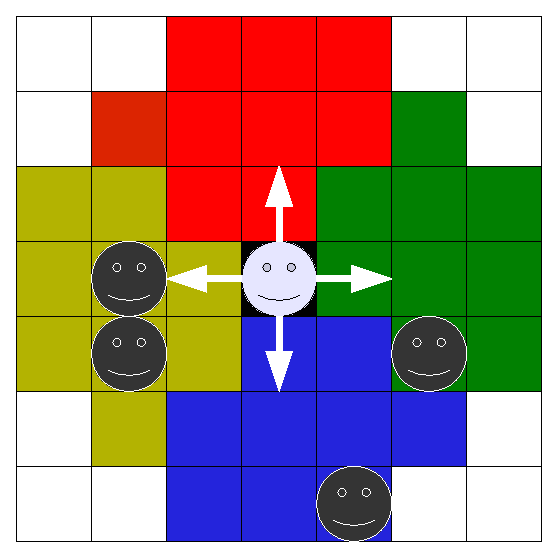
\includegraphics[width=0.45\columnwidth]{agent_random.eps}
}
\caption[Caption as shown in list of figures]{Agent bewegt sich in eine zuf\"allige Richtung (oder bleibt stehen)}
\label{agent_random:fig}
\end{figure}

\subsection{``Simple AI Agent''}
Ist der Zielagent in Sichtweite, bewegt sich dieser Agent auf das Ziel zu. Ist das Ziel nicht in Sichtweite, f\"uhrt er eine zuf\"allige Aktion aus.

\begin{figure}[htbp]
\centerline{	
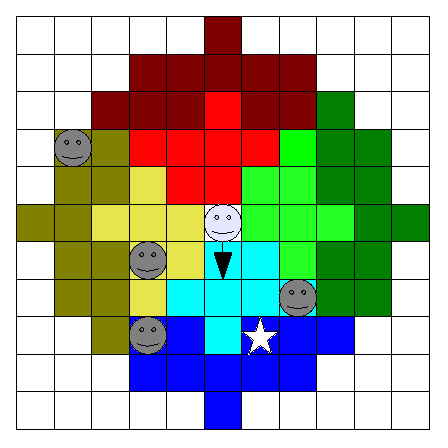
\includegraphics[width=0.45\columnwidth]{simple_agent_to_goal.eps}
}
\caption[Caption as shown in list of figures]{Agent bewegt sich auf Zielagent zu (sofern sichtbar)}
\label{simple_agent_to_goal:fig}
\end{figure}

\subsection{``Intelligent AI Agent''}
Ist der Zielagent in Sicht, verh�lt sich dieser Algorithmus wie ``Simple AI Agent''. Ist der Zielagent dagegen nicht in Sicht, wird versucht anderen Agenten auszuweichen um ein m\"oglichst breit gestreutes Netz aus Agenten aufzubauen. In der Implementation hei\ss{}t das, dass unter allen Richtungen, in denen kein anderer Agent geortet wurde, eine zuf\"allig ausgew\"ahlt wird. Falls alle Richtungen belegt (oder alle frei) sind, aus allen Richtungen eine zuf\"allig ausgew\"ahlt wird.

\begin{figure}[htbp]
\centerline{	
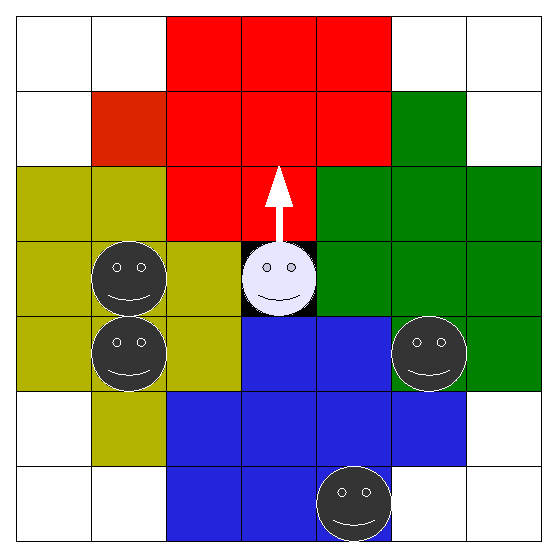
\includegraphics[width=0.45\columnwidth]{intelligent_agent.eps}
}
\caption[Caption as shown in list of figures]{Agent bewegt sich von anderen Agenten weg (falls Zielagent nicht sichtbar)}
\label{intelligent_agent:fig}
\end{figure}

\section{Grunds\"atzliche Zielagententypen}

Die Art der Bewegung des Zielagenten tr\"agt grunds\"atzlich zur Schwierigkeit eines Szenarios bei. Gemeinsam haben alle Arten von Bewegungen des Zielagenten, dass, wenn kein freies Feld zur Verf\"ugung steht, springt der Zielagent auf ein zuf\"alliges freies Feld auf dem Grid springt. Dies kommt einem Neustart gleich und ist notwendig um einer Verf\"alschung des Ergebnisses zu verhindern, das dadurch r\"uhren kann, dass ein oder mehrere Agenten (zusammen mit eventuellen Hindernissen) bis zum Ende des Problems alle vier Bewegungsrichtungen des Zielagenten blockieren.


\subsection{``Random Movement''}
Wie ``Randomized''. Sind alle m\"oglichen Felder belegt, wird wie oben beschrieben auf ein zuf\"alliges Feld gesprungen.

\subsection{``Total Random''}
Der Zielagent springt zu einem zuf\"alligen (freien) Feld auf dem Grid. Mit dieser Einstellung kann die Abdeckung des Algorithmus gepr\"uft werden, d.h. inwieweit die Agenten jeweils au\ss{}erhalb der \"Uberwachungsreichweite anderer Agenten bleiben. Jegliche Anpassung an die Bewegung des Zielagenten ist hier wenig hilfreich, ein Agent kann nicht einmal davon ausgehen, dass sich der Zielagent in der N\"ahe seiner Position der letzten Zeiteinheit befindet.

\subsection{``One direction change''}
Mit dieser Einstellung wird die der letzten Richtung entgegengesetzten Richtung aus der Menge der Auswahlm\"oglichkeiten entfernt und von den verbleibenden drei Richtungen (plus der Aktion ``Stehenbleiben'') eine zuf\"allig ausgew\"ahlt. Sind alle drei Richtungen versperrt, wird stehengeblieben.
War die letzte Aktion nicht eine Bewegungsrichtung sondern die Aktion ``Stehenbleiben'', so wird eine zuf\"allige Richtung ausgew\"ahlt. Sind alle Richtungen versperrt wird auch hier wie bei ``Random Movement'' auf ein zuf\"alliges Feld gesprungen.

\begin{figure}[htbp]
\centerline{	
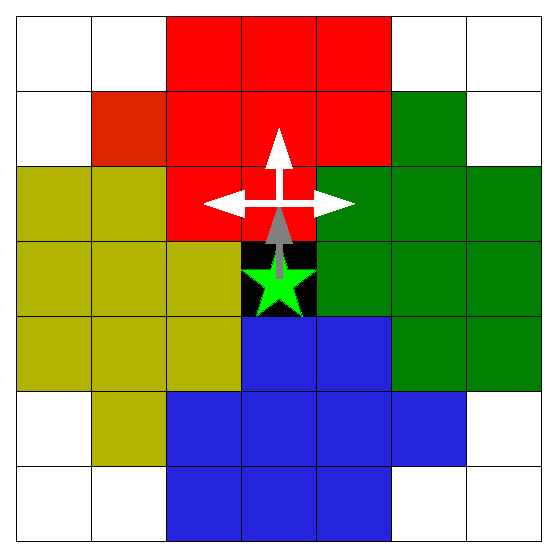
\includegraphics[width=0.45\columnwidth]{goal_direction_change.eps}
}
\caption[Caption as shown in list of figures]{Zielagent macht pro Schritt maximal eine Richtungs\"anderung}
\label{goal_agent_one_direction_change:fig}
\end{figure}

\subsection{``Always same direction''}
Der Zielagent versucht immer Richtung Norden zu gehen. Ist das Zielfeld blockiert, w\"ahlt er ein zuf\"alliges, angrenzendes, freies Feld im Westen oder Osten. Sind auch diese belegt, springt er wie oben auf ein zuf\"alliges freies Feld. Schafft es der Zielagent innerhalb von einer bestimmten Zahl (Breite des Spielfelds) von Schritten nicht, einen weiteren Schritt nach Norden zu gehen, wird ebenfalls gesprungen um ein Festh\"angen an einem Hindernis zu vermeiden.

\begin{figure}[htbp]
\centerline{	
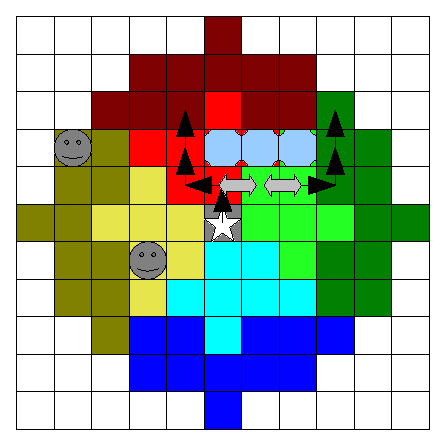
\includegraphics[width=0.45\columnwidth]{goal_always_same_direction.eps}
}
\caption[Caption as shown in list of figures]{Zielagent bewegt sich, wenn m\"oglich, immer nach Norden}
\label{goal_agent_always_same_direction:fig}
\end{figure}

\subsection{``Intelligent (Open)''}
Der Zielagent versucht andere Agenten zu vermeiden. Bei der Wahl der Richtung werden alle Richtungen gestrichen, in denen sich ein anderer Agent befindet. Von den verbleibenden Richtungen werden mit 20\% Wahrscheinlichkeit alle Richtungen gestrichen, in denen sich ein Hindernis befindet. Sind alle Richtungen gestrichen worden, bewegt der Zielagent sich zuf\"allig. Sind alle Richtungen blockiert, springt er wie in den anderen Einstellungen auch.

\begin{figure}[htbp]
\centerline{	
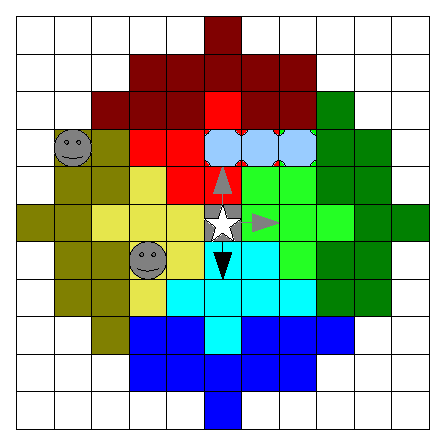
\includegraphics[width=0.45\columnwidth]{goal_intelligent_open.eps}
}
\caption[Caption as shown in list of figures]{Zielagent bewegt sich von Agenten und mit bestimmter Wahrscheinlichkeit von Hindernissen weg}
\label{goal_agent_intelligent_open:fig}
\end{figure}

\subsection{``Intelligent (Hide)''}
Der Zielagent vermeidet andere Agenten wie bei ``Intelligent (Open)'', streicht aber statt Richtungen mit Hindernissen Richtungen ohne Hindernisse mit 20\% Wahrscheinlichkeit.

\begin{figure}[htbp]
\centerline{	
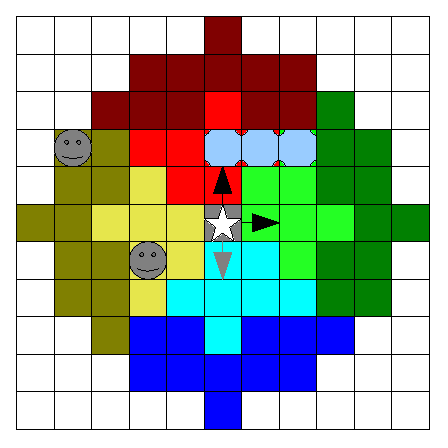
\includegraphics[width=0.45\columnwidth]{goal_intelligent_hide.eps}
}
\caption[Caption as shown in list of figures]{Zielagent bewegt sich von Agenten weg und mit bestimmter Wahrscheinlichkeit auf Hindernissen zu}
\label{goal_agent_intelligent_hide:fig}
\end{figure}

\subsection{``LCS''}
Eine LCS Implementierung die der der Implementierung eines LCS Agenten entspricht. Das Ziel des Zielagenten ist es hier aber, m\"oglichst nicht andere Agenten zu \"uberwachen (bzw. umgekehrt sich von anderen nicht \"uberwachen zu lassen, d.h. nicht in die \"Uberwachungsreichweite anderer Agenten zu geraten). Eine genaue Beschreibung folgt weiter unten.


\chapter{Szenarien}


Getestet werden eine Reihe von Szenarien (in Verbindung mit unterschiedlichen Werte f\"ur die Anzahl der Agenten, Gr\"o\ss{}e des Spielfelds und Art und Geschwindigkeit der Zielagentenbewegung). Wesentliche Rolle spielt hier die Verteilung der Hindernisse.

\section{Random Scenario}
Zwei Parameter bestimmen, wie das zuf\"allige Szenario auszusehen hat, zum einen der Prozentsatz an Hindernissen an der Gesamtzahl der Felder, zum anderen der Grad  inwieweit die Hindernisse zusammenh\"angen. Dieser Grad bestimmt nach Setzen eines Hindernisses die Wahrscheinlichkeit f\"ur jedes einzelne angrenzende freie Feld, dass dort sofort ein weiteres Hindernis gesetzt wird. Ein Wert von 0.0 ergibt somit ein v\"ollig zuf\"allig verteilte Menge an Hindernissen w\"ahrend ein Wert nahe eine oder mehrere stark zusammenh\"angende Strukturen schafft.
Wird der Prozentsatz an Hindernissen auf Null gesetzt, dann werden Hindernisse vollst\"andig deaktiviert. Als Optimierung werden in diesem Fall auch alle Sensorinformationen diesbez\"uglich deaktiviert. TODO optional

\begin{figure}[htbp]
\centerline{	
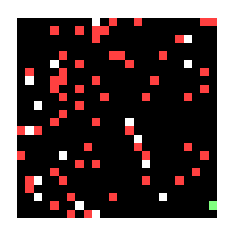
\includegraphics[width=0.45\columnwidth]{random_grid.eps}
}
\caption[Caption as shown in list of figures]{``Random Scenario'' : Zuf\"allige Verteilung von Hindernissen (rot), Agenten (weiss) und dem Zielagenten (gr\"un)}
\label{random_grid:fig}
\end{figure}

TODO BILDER von Grid mit verschiedenen Parametern
Percentage: 0.0, 0.1, 0.2, 0.3, 0.4
Connection Faktor: 0.01, 0.25, 0.5, 1.0

\section{Pillar Scenario}
Hier werden mit jeweils 7 Feldern Zwischenraum zwischen den Hindernissen (und mindestens 3 Feldern Zwischenraum zwischen Rand und den Hindernissen) Hindernisse verteilt. Idee ist, dass die Agenten eine kleine Orientierungshilfe besitzen aber gleichzeitig m\"oglichst wenig Hindernisse verteilt werden. TODO
Der Zielagent startet in der Mitte.

\begin{figure}[htbp]
\centerline{	
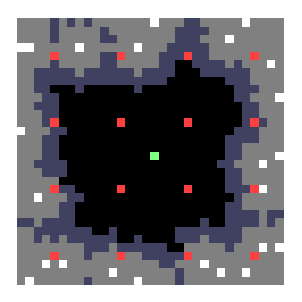
\includegraphics[width=0.45\columnwidth]{pillar_grid.eps}
}
\caption[Caption as shown in list of figures]{``Pillar Scenario'' : Regelm\"a\ss{}ig angeordnete Hindernisse (rot), zuf\"allige Verteilung von Agenten am Rand (weiss) und feste Startposition des Zielagenten in der Mitte(gr\"un)}
\label{pillar_grid:fig}
\end{figure}

\section{Cross Scenario}
Hier gibt es in der Mitte eine horizontale Reihe aus Hindernissen halber Gesamtbreite welche durch eine vertikale Reihe aus Hindernissen halber Gesamth\"ohe geschnitten wird.

\begin{figure}[htbp]
\centerline{	
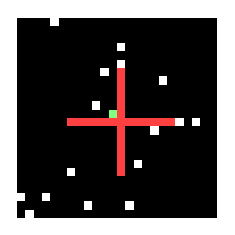
\includegraphics[width=0.45\columnwidth]{cross_grid.eps}
}
\caption[Caption as shown in list of figures]{``Cross scenario'' : Zentrierte, kreuzf\"ormige Anordnung der Hindernisse (rot), zuf\"allige Verteilung der Agenten (weiss) und dem Zielagenten (gr\"un) mit fester Startposition in der Mitte}
\label{cross_grid:fig}
\end{figure}

\section{Room scenario}
In der Mitte des Grids wird ein Rechteck der halben Gesamth\"ohe und -breite des Grids erstellt, welches eine \"Offnung von 4 Feldern Breite aufweist. Der Zielagent startet wie im Pillar Scenario in der Mitte, alle Agenten starten am Rand des Grids.

\begin{figure}[htbp]
\centerline{	
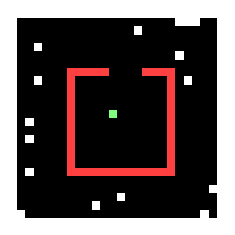
\includegraphics[width=0.45\columnwidth]{room_grid.eps}
}
\caption[Caption as shown in list of figures]{``Room Scenario'' : Zentrierte, quaderf\"ormige Anordnung der Hindernisse (rot) mit \"Offnung oben, zuf\"allige Verteilung der Agenten (weiss) am Rand und der Zielagenten (gr\"un) mit festem Startpunkt in der Mitte}
\label{room_grid:fig}
\end{figure}


\section{Difficult Scenario}
Hier wird das Grid zum einen an der rechten Seite vollst\"andig durch Hindernisse blockiert um den Torus zu halbieren. Alle Agenten starten am linken Rand, der Zielagent startet auf der rechten Seite.
In regelm\"a\ss{}igen Abst\"anden (7 Felder Zwischenraum) befindet sich eine vertikale Reihe von Hindernissen mit \"Offnungen von 4 Feldern Breite abwechselnd im oberen Viertel und dem unteren Viertel.

\begin{figure}[htbp]
\centerline{	

\includegraphics[width=0.45\columnwidth]{difficult_grid.eps}
}
\caption[Caption as shown in list of figures]{``Difficult Scenario'' : Feste, wandartige Verteilung von Hindernissen (rot) in regelm\"a\ss{}igen Abst\"anden mit \"Offnungen, Agenten (weiss) mit zuf\"alligem Startpunkt am linken Rand und dem Zielagenten (gr\"un) mit festem Startpunkt rechts oben}
\label{difficult_grid:fig}
\end{figure}


TODO vielleicht Agentenl\"osungen eines Szenarios in das andere einsetzen?

\chapter{Ablauf der Simulation}

Bei Simulationen am Computer stellt sich sofort die Frage nach der Genauigkeit. Die Agenten werden bei dieser Simulation nacheinander abgearbeitet und bewegen sich auf einem diskreten Grid. Dies kann u.U. dazu f\"uhren, dass je nach Position in der Liste abzuarbeitender Agenten die Informationen \"uber die Umgebung unterschiedlich alt sind. Die gro\ss{}e Frage ist deshalb, in welcher Reihenfolge Sensordaten ermittelt, ausgewertet, Agenten bewegt, intern sich selbst bewertet und global die Qualit\"at gemessen wird.
Einzige Restriktionen sind, dass eine Aktion nach der Verarbeitung der Sensordaten stattfinden muss und eine Bewertung einer Aktion nach dessen Ausf\"uhrung stattfinden muss. Ansonsten gibt es folgende M\"oglichkeiten:

\section{Reihenfolge der Ausf\"uhrung}
\begin{enumerate}
\item F\"ur alle Agenten werden erst einmal die neuen Sensordaten erfasst und sich f\"ur eine Aktion entschieden. Sind alle Agenten abgearbeitet werden die Aktionen ausgef\"uhrt.
\item Die Agenten werden nacheinander abgearbeitet, es werden jeweils neue Sensordaten erfasst und sich sofort f\"ur eine neue Aktion entschieden. 
\end{enumerate}

Bei der ersten M\"oglichkeit haben alle Agenten die Sensordaten vom Beginn der Zeiteinheit, w\"ahrend bei der zweiten M\"oglichkeit sp\"ater verarbeitetere Agenten bereits die Aktionen der bereits berechneten Agenten miteinbeziehen k\"onnen. Umgekehrt k\"onnen dann fr\"uhere Agenten bessere Positionen fr\"uher besetzen. Da aufgrund der primitiven Sensoren nicht davon auszugehen ist, dass Agenten beginnende Bewegungen (und somit deren Zielposition) anderer Agenten einbeziehen k\"onnen, soll jeder Agent von den Sensorinformationen zu Beginn der Zeiteinheit ausgehen.
Die Reihenfolge der Ausf\"uhrung der Aktionen spielt eine Rolle, wenn mehrere Agenten sich auf das selbe Feld bewegen wollen. Arbeiten wir die Liste unserer Agenten einfach linear ab, haben vorne stehende Agenten eine h\"ohere Wahrscheinlichkeit, dass ihre Aktion ausgef\"uhrt wird. Da es keine Veranlassung gibt, ihnen diesen Vorteil zu geben, werden Aktionen in zuf\"alliger Reihenfolge abgearbeitet. Bez\"uglich der Bewegung ergibt sich hierbei eine weitere Frage, n\"amlich wie unterschiedliche Bewegungsgeschwindigkeiten behandelt werden sollen. Alle Agenten haben eine Einheitsgeschwindigkeit von maximal einem Feld pro Zeiteinheit, w\"ahrend sich der Zielagent je nach Szenario gleich eine ganze Anzahl von Feldern bewegen kann. Auch hier habe ich mich f\"ur eine zuf\"allige Verteilung entschieden. Kann sich der Zielagent um n Schritte bewegen, so wird seine Bewegung in \(n\) Einzelschritte unterteilt, die nacheinander mit zuf\"alligen Abst\"anden (d.h. Bewegungen anderer Agenten) ausgef\"uhrt werden.
Eine weitere Frage ist, wie der Zielagent diese weiteren Schritte festlegen soll. Hier soll ein Sonderfall eingef\"uhrt, so dass der Zielagent in einer Zeiteinheit mehrmals (\(n\)-mal) neue Sensordaten erfassen und sich f\"ur eine neue Aktion entscheiden kann.

\section{Reihenfolge Rewardverteilung}
Schlie\ss{}lich bleibt die Frage danach, wann gepr\"uft werden soll, ob der Zielagent in Sicht ist, und wann somit der Reward verteilt wird. Da XCS in der Standardimplementation darauf ausgelegt ist, den Reward jeweils genau einer Aktion zuzuordnen, sollte der Reward nicht bei jeder einzelnen Bewegung des Zielagenten \"uberpr\"uft und verteilt werden, sondern nur einmal pro Zeiteinheit. Au\ss{}erdem soll der Einfachheit halber der Reward auch von bin\"arer Natur sein (�Zielagent in \"uberwachungsreichweite� oder �Zielagent nicht in \"uberwachungsreichweite�), weshalb Zwischenzust\"ande f\"ur den Reward (z.B. �War zwei von drei Zeitschritten in der \"uberwachungsreichweite� => 2/3 Reward) ausgeschlossen werden sollen. F\"ur den Reward gibt es somit folgende M\"oglichkeiten:

\begin{enumerate}
\item Rewards werden direkt nach der Ausf\"uhrung einer einzelnen Aktion vergeben
\item Rewards werden nach Ausf\"uhrung aller Aktionen der Agenten vergeben
\item Rewards werden nach Ausf\"uhrung aller Aktionen des Zielagenten vergeben
\end{enumerate}

Werden die Rewards sofort vergeben (Punkt 1), dann werden sich sp\"ater noch weg-bewegende bzw. sich sp\"ater noch hin-bewegende Agenten nicht beachtet. Da die Agenten in zuf\"alliger Reihenfolge abgearbeitet werden, w\"urde das bedeuten, dass die Bewegung der restlichen (zuf\"alligen) Anzahl von Agenten in den Reward nicht miteinbezogen wird. Selbiges gilt f\"ur Punkt 3. 
Auch der Zielagent kann Reward erhalten. Hierbei gibt es ebenfalls drei M\"oglichkeiten:
\begin{enumerate}
\item Reward direkt nach Ausf\"uhrung des letzten Schritts
\item Reward nach Ausf\"uhrung aller Agenten
\end{enumerate}

Eine konkrete Antwort kann man auf diese zwei Fragen nicht geben, sie h\"angt n\"amlich davon ab, was man denn nun eigentlich erreichen m\"ochte, also auf welche Weise die Qualit\"at des Algorithmus bewertet wird. Der naheliegendste Messzeitpunkt ist nachdem sich alle Agenten bewegt haben. Da wir Agenten und Zielagenten in einem Durchlauf gemeinsam bewegen, stellt sich die Frage nicht, ob wir wom\"oglich vor der Bewegung des Zielagenten die Qualit\"at messen sollen. Eine Messung nach der Bewegung des Zielagenten w\"urde diesem erlauben, sich vor jeder Messung optimal zu positionieren, was in einer geringeren Qualit\"at f\"ur den Algorithmus resultiert, da sich der Zielagent aus der \"Uberwachungsreichweite anderer Agenten hinausbewegen kann. Letztlich ist es eine Frage der Problemstellung, denn eine Messung nach Bewegung des Zielagenten bedeutet letztlich, dass ein Agent, einen gerade aus seiner \"Uberwachungsreichweite heraus laufenden Zielagenten in diesem Schritt nicht mehr \"uberwachen kann.
Da ein wesentlicher Bestandteil die Kooperation (und somit die Abdeckung des Spielfelds anstatt dem Verfolgen des Zielagenten) sein soll, soll ein Bewertungskriterium sein, inwieweit der Einfluss des Zielagenten minimiert werden soll. Auch findet, wenn wir vom realistischen Fall ausgehen, die Bewegung des Zielagenten gleichzeitig mit allen anderen Agenten statt. Die Qualit\"at wird somit nach der Bewegung des Zielagenten gemessen. Die \"Uberlegung unterstreicht auch nochmal, dass es besser ist, den Zielagenten insgesamt wie einen normalen (aber sich mehrmals bewegenden) Agenten zu behandeln.
Was den Zeitpunkt des Rewards betrifft, lautet die Hypothese, dass wir ein besseres Ergebnis erreichen, wenn man den Reward anhand der selben Momentaufnahme verteilt, anhand der wir auch die Qualit\"at testen, d.h. dass Punkt 2 Punkt 1 \"uberlegen ist. Dies best\"atigt sich in Tests siehe TODO.

\section{Zusammenfassung}
Zusammenfassend sieht der Ablauf aller Agenten (inklusive des Zielagenten) also wie folgt aus:

\begin{figure}[H]
\setbox0\vbox{\small
\begin{enumerate}
\item Erfassung aller Sensordaten
\item Wahl der Aktion anhand der Regeln des jeweiligen Agenten
\item Ausf\"uhrung der Aktion (in zuf\"alliger Reihenfolge, der Zielagent f\"uhrt nach dem ersten Schritt au\ss{}erdem Schritt 1. und 2. f\"ur alle weiteren Schritte nochmals durch)
\item Bestimmung des Rewards
\item Bestimmen der Qualit\"at dieser Zeiteinheit
\end{enumerate}
}
\centerline{\fbox{\box0}}
\end{figure}

\chapter{Erste Analyse der Agenten ohne LCS}

In diesem Kapitel sollen erste Analysen bez\"uglich der verwendeten Szenarien anhand des zuf\"alligen Algorithmus, des Algorithmus mit einfacher Intelligenz (``Simple AI Agent'') und des Algorithmus mit komplexerer Regeln (``Intelligent AI agent'') angefertigt werden. Die Ergebnisse aus der Analyse werden eine Grundlage f\"ur die vergleichende Betrachtung der Agenten mit LCS Algorithmen dienen.

\section{Total Random Goal Agent Movement}

In allen Szenarien mit dieser Form der Bewegung des Zielagenten kommt es nur darauf an, dass die Agenten einen m\"oglichst gro\ss{}en Bereich des Grids abdecken. In allen Standardszenarios zeigt sich, dass der ``Simple AI Agent'' sich wie erwartet nicht wesentlich vom zuf\"alligen Agenten unterscheidet. 

\subsection{Ohne Hindernisse}

Ohne Hindernisse gibt sich ein klares Bild. Das Ergebnis der einfachen KI ist etwas schlechter als der des zuf\"alligen Agenten, da sich immer wenn mehrere Agenten den Zielagenten in der selben Richtung in Sichtweite haben, sich mehrere Agenten in die selbe Richtung bewegen. Dies beeintr\"achtigt die zuf\"allige Verteilung der Agenten auf dem Spielfeld und f\"uhrt somit auch zu einer niedrigeren Abdeckung des Grids.
Der intelligente Agent liegt hier sehr deutlich vorne, ein m\"oglichst weitr\"aumiges Verteilen auf dem Feld f\"uhrt zum Erfolg, denn genau das wird mit dem v\"ollig zuf\"allig springenden Agenten getestet.

\subsection{Zuf\"allig verteilte Hindernisse}

Hier ergeben sich bei allen Einstellungen des ``Connection Factors'' und ''Obstacle Factors'' ebenfalls ein klares Bild, der intelligente Agent liegt wieder vorne, dann kommt allerdings schon der einfache Agent mit bis zu 10\% zum zuf\"alligen Agenten. Der wesentliche zweite Faktor ist hier, dass der einfache Agent, wenn er den Zielagenten in Sicht hat, davon ausgehen kann, dass sich in dieser Richtung wahrscheinlich kein Hinderniss befindet, w\"ahrend der zuf\"allige Agent Hindernisse \"uberhaupt nicht beachtet, somit \"ofters gegen ein Hinderniss l\"auft und letztlich \"ofters stehen bleibt. Der Unterschied zwischen beiden Agenten ist besonders hoch in Szenarien mit gr\"o\ss{}erem Anteil an Hindernissen.
Ansonsten liegt der intelligente Agent wieder eindeutig vorne, beherrscht aber besonders gut Szenarien hohem ``Connection Factor'' (\(1.0\)) der geringem Anteil an Hindernissen (\(0.1\)), bei denen er bis zu etwa 15\% \"uber dem Ergebnis des einfachen Agenten liegt.
Dies liegt daran, dass Szenarien mit hohem ``Connection Factor'' bedeuten, dass alle Hindernisse zusammenh\"angend einen gro\ss{}en Block bilden und somit dem Szenario ohne Hindernissen \"ahnlich sind, auf dem dieser Agent ja besonders gut abschneidet. In zerkl\"uftete Szenarien hat der Algorithmus dagegen Schwierigkeiten um andere Agenten \"uberhaupt zu Gesicht bekommen, der Vorteil der Verteilung f\"allt also zu einem Teil weg. 

Dies best\"atigt auch ein Durchlauf bei dem Sichtbehinderungen durch Hindernisse deaktiviert sind. Hierbei erreicht der intelligente Agent im Szenario (\(0.4\), \(0.1\)) statt TODO evtl weg

\section{Random Neighbor und One Direction Change}

Wesentlicher Punkt bei beiden Szenarien ist, dass der jetzige Ort des Zielagenten maximal zwei Felder (die Standardgeschwindigkeit des Zielagenten in den Tests) vom Ort in der vorangegangenen Zeiteinheit entfernt ist. Somit ist ein lokales Einfangen eher von Relevanz, wenn auch der Zielagent grunds\"atzlich schneller als andere Agenten ist.

Dementsprechend ist der einfache Agent bei einem Hinderniss-Anteil von \(0.0\) bis \(0.1\) besser als alle anderen Agenten und dementsprechend ist bei allen Tests der zuf\"allige Agent weit abgeschlagen.
Ab einem Anteil von \(0.2\) liegt jedoch der intelligente Agent vorne. Dies liegt schlicht an der Zahl der Agenten relativ zur hindernissfreien Fl\"ache, da sich die Agenten in m\"oglichst gro\ss{}em Abstand zueinander positionieren.

Im Falle des ``One Direction Change'' bewegt sich der Agent im Grunde nur etwas schneller, da er es vermeidet, auf das urspr\"ungliche Feld zur\"uckzukehren.
TODO? Vielleicht sogar Random Neighbor raus...

\section{Intelligent Open}

\section{Intelligent Hide}

TODO:Beide gleiche Ergebnisse?Source pr\"ufen


\section{Always Same Direction}

TODO

\section{LCS}

Wird weiter unten besprochen.





\section{Zusammenfassung}

Wie wir gesehen haben gibt es also Szenarien in denen Abdeckung kaum eine Rolle spielt und lokale Entscheidungen eine wesentliche Rolle spielen. Dies wird es erleichtern, geeignete Szenarien im Kapitel ``Kommunikation'' zu finden.




TODO Anpassung LCS an unterschiedliche Sichtreichweiten?



\chapter{LCS}

\section{Einf\"uhrung}

Jeder Agent besitzt ein Learning Classifier System, welches auf dem von Butz TODO XCS basiert. Die Implementierung entspricht im Wesentlichen der Standardimplementation von Butz 2000, eine Besonderheit stellt allerdings die Problemdefinition dar. Keine der gegenw\"artigen Implementationen und Varianten von XCS besch\"aftigen sich mit dynamischen \"Uberwachungsszenarios sondern mit Szenarios, bei denen das Ziel in einer statischen Umgebung gefunden werden muss. 

Im XCS-Multistepverfahren (TODOLiteratur) l\"auft ein Problem so lange bis ein positiver Reward aufgetreten ist und startet dann das Szenario neu. Bei einem \"Uberwachungsszenario mit kontinuierlichem Reward ist das Multistepverfahren nicht anwendbar, das Szenario kann nicht neugestartet werden, da sich die Agenten w\"ahrend des Laufs anpassen sollen. Ziel ist hier ja nicht, einen bestimmten Weg zu einem festen Ziel zu finden (wie z.B. bei WOODS TODO), sondern eine bestimmte Regelmenge zu erlernen, mit der eine m\"oglichst gute, dauerhafte \"Uberwachung stattfinden kann. 

In der hier verwendeten Implementierung l\"auft das Problem deshalb einfach weiter. Wesentlicher Unterschied zu XCS wird deshalb die Behandlung des Rewards sein.

In der Literatur fehlen Arbeiten, in denen ein solches Szenario (ohne globale Steuerungseinheit oder Regeltausch) in Verbindung mit dem XCS behandelt wird. Diese Arbeit soll diese L\"ucke schlie\ss{}en und die Basis f\"ur weitere Arbeiten in dieser Richtung liefern.


TODO anfaengliche Initialisierung?

\section{Classifier}

Ein LCS beinhaltet eine Reihe von Classifiern. Ein einzelner Classifier besteht im Wesentlichen aus f\"unf Teilen:

\subsection{Fitness}
Der Fitness Wert soll die allgemeine Genauigkeit des Classifiers 
repr\"asentieren und wird \"uber die Zeit hinweg sukzessive an die beobachteten Rewards angepasst. TODO Wilson. Der Wertebereich verl\"auft zwischen \(0.0\) und \(1.0\) (maximale Genauigkeit).

\subsection{Prediction}
Der ``Prediction''-Wert des Classifiers stellt die H\"ohe des Rewards dar, von dem der Classifier vermutet, dass er ihn bei der n\"achsten Vergabe des Rewards erhalten wird. Auch dieser Wert wird stetig angepasst.

\subsection{Prediction Error}
Der �Prediction-Error�-Wert soll die Genauigkeit des Classifiers bzgl. der Reward-Prediction (durchschnittliche Differenz zwischen Prediction und tats\"achlichem Reward) repr\"asentieren. U.a. auf Basis dieses Werts wird der Fitness-Wert des Classifiers angepasst.

\subsection{Aktion}
Wird ein Classifier ausgew\"ahlt, wird eine bestimmte Aktion ausgef\"uhrt. In unserem Szenario entsprechen die Aktionsm\"oglichkeiten die der anderen Agenten, also 4 Bewegungsrichtungen plus eine ``nichts-tun''-Aktion.

\subsection{Kondition}
Die Kondition gibt an, bei welchem Sensor-Input dieser Classifier ausgew\"ahlt werden kann. 

\section{Sensoren und Matching}

In der hier verwendeten Implementierung gibt es zwar eine gewisse Vorverarbeitung der Sensordaten, im Wesentlichen m\"ussen aber Kondition und Sensordaten \"ubereinstimmen, damit der jeweilige Classifier ausgew\"ahlt wird. Konkret besteht die Kondition ebenfalls aus einem 9-stelligen Vektor, der allerdings nicht nur bin\"are sondern trin\"are Werte besitzen kann. 

\subsection{Wildcards}

Neben den zu den Sensordaten korrespondierenden Werten 0 und 1 gibt es noch einen dritten ``dont-care''-Zustand ``\#'', der anzeigen soll, dass beim Vergleich zwischen Kondition und Sensordaten diese Stelle ignoriert werden soll. Eine aus nur ``dont-care'' Werten bestehende Kondition w\"urde somit bei der Auswahl immer in Betracht gezogen werden, da er auf alle Sensor-Inputs passt.

Beispiel:
Kondition \(1.\#010.1\#01\) matched Sensordaten \(1.0010.1001\), \(1.1010.1001\), \(1.0010.1101\) und \(1.1010.1101\).

Die Benutzung von Wildcards erlaubt es dem LCS mehrere Classifier zu subsummieren, wodurch die Gesamtzahl der Classifier sinkt und somit Erfahrungen, die ein LCS Agent sammelt, nicht unbedingt doppelt gemacht werden m\"ussen. Die dahinter stehende Annahme ist, dass es Situationen gibt, in denen ein Wert aus dem Sensor-Input f\"ur die Qualit\"at der Entscheidung weniger entscheidend sein kann, als die Ersparnis durch das Zusammenlegen beider Classifier, d.h. dem Ignorieren dieses Inputs.

\subsection{Matching von Sensordaten mit Classifiern}

Beim Vergleich mit Sensordaten wir ebenfalls mit einem Vektor wie bei \(B\) erglichen. Entscheidend beim Vergleich ist hier aber nicht, dass beide Vektoren identisch sind, sondern, dass der Classifier ``matched''. Ein Element des Bedingungsvektors kann 3 Zust\"ande einnehmen. \(0\), \(1\) und \(\#\). \(\#\) beinhaltet beide Zust\"ande \(0\) und \(1\).

Den dritten verwendeten Vergleich zwischen Bedingungsvektoren gibt es bei der Subsumation (der Kinder zu ihren Eltern und des gesamten ActionSets siehe ~(\ref{sec:subsummation}). Ein Classifier subsumiert einen anderen Classifier, wenn er ihn beinhaltet, aber nicht identisch mit ihm ist, also allgemeiner ist.

\subsection{Drehungen}

Ein Classifier besteht aus dem Bedingungsvektor \[(g x_{0} x_{1} x_{2} x_{3})\] (bzw. \[(g x_{0} x_{1} x_{2} x_{3} y_{0} y_{1} y_{2} y_{3})\] f\"ur den Fall mit Hindernissen) und der Aktion \(a\).

Eine wesentliche Vereinfachung, die angenommen wird, ist, dass angenommen wird, dass eine Aktion in einer anderen, in 90 Grad Schritten gedrehten Umwelt, gleiche G\"ute besitzt.
In einer statischen Umgebung ist dies nicht unbedingt der Fall, ohne diese Vereinfachung k\"onnte sich ein Agent einfacher zurechtfinden, wie TODO (keine Drehung, 1 Problem pro Experiment) diese Testl\"aufe zeigen.
Da wir uns aber auf den dynamischen Fall konzentrieren und durch diese Vereinfachung eine signifikante Verkleinerung des Suchraums erreichen, benutzen wir die Vereinfachung.
Im Algorithmus betrifft dies prim\"ar den Vergleich von Classifiern untereinander und mit dem Sensorstatus. 

\subsection{\"Aquivalenz von Classifiern}
Ein Classifier A ist identisch mit einem Classifier B wenn gilt:

\begin{enumerate}
\item \[A_{g} = B_{g}\]
\item Falls \[A_{g} = 0\]:

\begin{enumerate}
\item Es gibt ein \(i\) f\"ur das gilt: \[(A_{x_{0+i \bmod 4}} A_{x_{1+i \bmod 4}} A_{x_{2+i \bmod 4}} A_{x_{3+i \bmod 4}}) = (B_{x_{0}} B_{x_{1}} B_{x_{2}} B_{x_{3}})\]
\item Mit Hindernissen muss f\"ur dieses \(i\) au\ss{}erdem gelten: 

\begin{enumerate}
\item \[(A_{y_{0+i \bmod 4}} A_{y_{1+i \bmod 4}} A_{y_{2+i \bmod 4}} A_{y_{3+i \bmod 4}}) = (B_{y_{0}} B_{y_{1}} B_{y_{2}} B_{y_{3}}\]
\item Falls \(A_{a} = \mathrm{NO_ACTION}\): \[A_{a} = B_{a}\]
\item Falls \(A_{a} \neq \mathrm{NO_ACTION}\): \[(A_{a}+i) \bmod 4 = B_{a}\]
\end{enumerate}
\end{enumerate}

\item Falls \(A_{g} = 1\):

\begin{enumerate}
\item \[(A_{x_{0}} A_{x_{1}} A_{x_{2}} A_{x_{3}}) = (B_{x_{0}} B_{x_{1}} B_{x_{2}} B_{x_{3}})\]
\item Mit Hindernissen muss au\ss{}erdem gelten: \[(A_{y_{0}} A_{y_{1}} A_{y_{2}} A_{y_{3}}) = (B_{y_{0}} B_{y_{1}} B_{y_{2}} B_{y_{3}})\]
\item \[A_{a} = B_{a}\]
\end{enumerate}

\end{enumerate}

Die Gleichheit zwischen Vektoren gilt, wenn paarweise Gleichheit zwischen den Elementen besteht, also \(A_{x_{i}} = B_{x_{i}}\) f\"ur \(i = 0 \dots 3\) und \(A_{y_{i}} = B_{y_{i}}\) f\"ur \(i = 0 \dots 3\) im Fall mit Hindernissen.

\subsection{Test Drehungen}

Mit aktivierter Optimierung der Drehungen wird in bestimmten Szenarien bis zu einer bestimmten Schrittzahl ein besseres Ergebnis erreicht, d.h. die Konvergenzgeschwindigkeit wird erh\"oht. In l\"angeren Durchl\"aufen mit gr\"o\ss{}erer Schrittzahl werden jedoch bessere Ergebnisse ohne der Optimierung erreicht. Der Zugewinn folgt aus einer durch die zus\"atzliche lokale Information die in den Classifiern gespeichert werden kann.

In einer zuk\"unftigen Implementierung sollte \"uberlegt werden, wie bei r\"aumlichen Aufgaben f\"ur Classifier ein LCS sowohl drehbare als auch nicht-drehbare Classifier speichern kann. Dies kann in einer Form des erw\"ahnten Wildcard-Systems bewerkstelligt werden. Dadurch und zusammen mit der Subsummation k\"onnten beide Vorteile vereint werden und sowohl lokale, als auch allgemeine Information gesammelt werden. TODOvielleicht doch noch rein?




\section{Implementation}

F\"ur die Auswahl der tats\"achlich auszuf\"uhrenden Aktion m\"ussen dann alle (genotypischen) Classifier in AppliedClassifier umgewandelt werden, die jeweils genau auf eine bestimmte Aktion verweisen.
Sichtwe

Zur Durchf\"uhrung und Forschung war es notwendig, den kompletten XCS Algorithmus nachvollziehen zu k\"onnen. TODO

Besonders die Verwaltung der Numerosity und die Verwendung des maxPrediction TODO


Das Multistepverfahren baut darauf auf, dass die Qualit\"at der Agenten sich sukzessive mit jeder Probleminstanz verbessert, der Reward eben an immer weiter vom Ziel entfernte Aktionen TODO weitergereicht wird.

Der hier entwickelte Algorithmus muss prim\"ar nicht einen Weg zum Ziel erkennen, sondern eine m\"oglichst optimale (und auch an andere Agenten angepasste) Verhaltensstrategie finden.

Da sich das Ziel schneller bewegt, kann eine einfache Verfolgungsstrategie nicht zum Erfolg f\"uhren. Eine einfache Implementation mit einem simplen Agenten der auf das Ziel zugeht, wenn es in Sicht ist und sich sonst wie ein sich zuf\"allig bewegender Agent verh\"alt, schneidet grunds\"atzlich schlechter ab.


\subsection{Numerosity}



TODO Beschreibung
In der originalen Implementierung von Butz 2000 TODO war die Behandlung der Numerosity stark optimiert auf den Fall des einmaligen Rewards ohne Protokollierung der bisherigen ActionSets. Nach einer missgl\"uckten ersten Implementierung � der Wert der numerositySum eines ClassifierSets stimmte nicht mehr mit der Summe der numerosity-Werte der enthaltenen Classifiers \"uberein � entschloss ich mich den entsprechenden Code neuzuschreiben. Hierbei wurde jedem Classifier eine Liste der Eltern, d.h. der jeweiligen ActionSets, zugewiesen.
Wird ein Microclassifier entfernt, wird dann lediglich die \"Anderungsfunktion der Numerosity des Classifiers aufgerufen, der dann wiederum die NumerositySum der jeweiligen Eltern anpasst. Dies macht einige Optimierungen r\"uckg\"angig, erspart aber sehr viel Umst\"ande, die NumerositySum immer auf den aktuellen Stand zu halten.
Positiver Nebeneffekt ist, dass man dadurch leicht auf die Menge der ActionSets zugreifen kann, denen ein Classifier angeh\"ort. Inwiefern das tats\"achlich von Nutzen sein kann ist offen. TODO
Kernst\"uck des LCS Agenten:



\subsection{Covering}

Die Implementation entspricht im Wesentlichen dem Original, es wurde aber im Hinblick auf eine klare Code-Struktur eine Optimierung entfernt und Code zur Behandlung von Drehungen hinzugef\"ugt. Im Original wird die Erstellung des MatchSets gleichzeitig mit dem Covering ausgef\"uhrt, wodurch m\"oglicherweise Zeit gespart wird, w\"ahrend in dieser Implementierung es in zwei Funktionen aufgeteilt wurde. TODOBEschreibung
Bez\"uglich der Drehung musste eine Schleife eingef\"ugt werden, die die abgedeckten Aktionen mit allen, inklusive durch Drehung entstandenen, Aktionen eines Classifiers aktualisiert. Ein einzelner Classifier kann also mehrere Aktionen abdecken, beispielsweise kann ``0-0000-0000->0'' bei der Sensoreingabe ``0-0000-0000'' alle vier Aktionen bereits abdecken. TODO besseres Beispiel. 


In meiner ersten Version hatte ich alle ung\"ultigen Aktionen von vornherein f\"ur das Covern ausgeschlossen. Eine ung\"ultige Aktion ist beispielsweise ein Laufen gegen ein Hindernis oder einen Agenten. Alleine dadurch verbesserte sich die Leistung um etwa 0.5\%. Das l\"asst sich darauf zur\"uckf\"uhren, dass die Sensoren eines Agenten eigentlich nur feststellen k\"onnen, ob ein anderer Agent in Sichtweite ist, nicht aber in welcher Entfernung. F\"ur die eigentlichen Ergebnisse wurde die daf\"ur verantwortliche Methode wieder entfernt.

Au\ss{}erdem ist ein Fehler der originalen XCS Implementation behoben. Wenn neue Classifier beim Covering hinzugef\"ugt werden, wird ihre anf\"angliche ActionSetSize auf die numerositySum des matchSets gesetzt. Einen Grund daf\"ur gibt es nicht, in meiner Implementation setze ich deshalb den Wert auf die anf\"angliche Gr\"o\ss{}e des actionSets.
Beim Aufruf des Covering-Algorithmus weiss man schon, wie gro\ss{}

TODO nein!


\subsection{Subsummation}\label{sec:subsummation}

Ein Problem ist hier nat\"urlich die Sicherstellung, dass Informationen nicht verloren gehen. Andere Arbeiten befassen sich mit der Untersuchung von der Benutzung von Wildcards. In der hier verwendeten Implementation \"ubernehme ich unver\"andert die Implementation aus der Literatur.

\subsection{Evolution\"arer Algorithmus}

Der genetische Algorithmus wurde im Wesentlichen nicht ver\"andert. Da aber die Bin\"arsensoren eng zusammenh\"angen, werden beim Crossing Over zwei feste Stellen f\"ur Crossing Over benutzt. Die Stellen trennen somit die 3 Gene, Zielagent, Agenten und feste Hindernisse.

Im Test erbrachte die Benutzung des Algorithmus wenig Unterschied.
TODO Erkl�rung


\section{Ablauf eines LCS}

\begin{enumerate}
\item Bei der Auswahl einer Aktion werden zuerst einmal alle Classifier mit denjenigen Konditionen gesucht, die auf die aktuellen Sensordaten passen. Diese bilden dann das MatchSet.
\item Im n\"achsten Schritt w\"ahlen wir einen Classifier aus diesem MatchSet aus und speichern dessen Aktion.
\item Schlie\ss{}lich bilden wir anhand des MatchSets und der gew\"ahlten Aktion das ActionSet
\end{enumerate}

\subsection{Exploration and Exploitation}

Die Auswahl in Punkt (2) kann auf verschiedene Weise erfolgen. In XCS gibt es drei M\"oglichkeiten der Auswahl, wobei man zus\"atzlich noch w\"ahrend eines Experiments zwischen den M\"oglichkeiten wechseln kann.
\begin{enumerate}
\item ``exploit'': Es wird immer ein Classifier mit dem h\"ochsten Produkt aus fitness \(*\) prediction gew\"ahlt
\item ``explore'': Es wird mit Hilfe einer Roulette-Auswahl, welche anhand des Produkts aus fitess \(*\) prediction geordnet ist, ein Classifier ausgew\"ahlt
\item ``random-explore'': Es wird ein zuf\"alliger Classifier gew\"ahlt, unabh\"angig von fitness oder prediction.
\end{enumerate}

In der XCS Implementierung sind alle drei M\"oglichkeiten zu finden, standardm\"a\ss{}ig ist jedoch M\"oglichkeit 2 zugunsten von M\"oglichkeit 3 deaktiviert.
Bei einem dynamischen \"Uberwachungsszenario ist es im Vergleich zu standardm\"a\ss{}igen statischen Szenarien weder n\"otig noch hilfreich ``random-explore'' zu nutzen. Die Idee f\"ur ``random-explore'' in einem statischen Szenario ist, dass man vermeiden m\"chte, dass das LCS immer wieder die selben Entscheidungen trifft und somit immer wieder den selben Umweltreizen ausgesetzt ist, was wiederum zu immer wieder gleichen Entscheidungen f\"uhrt usw.
Bei einem dynamischen Szenario ergibt sich das Problem nicht, andere Agenten und das Ziel sind in stetiger Bewegung und der eigene Startpunkt ist nicht fixiert. Das gewichtete ``explore'' oder gar nur ``exploit'' sollten deshalb ausreichen, wenn nicht sogar wesentlich besser abschneiden.

\subsection{Wechsel zwischen Exploration und Exploitation}

In der Standardimplementierung von XCS wird zwischen ``exploit'' und ``random-explore'' nach jedem Erreichen des Ziels umgeschalten. 

M\"oglichkeit (3.) entspricht dem Fall in der Standardimplementierung von XCS. Dabei wird bei jedem Erreichen eines positiven Rewards zwischen ``explore'' und ``exploit'' hin und hergeschaltet, was in der Standardimplementierung dem Beginn eines neuen Problems entspricht.

Hierbei gibt es mehrere verschiedene M\"oglichkeiten:

\begin{enumerate}
\item Immer ``exploit''
\item Immer ``explore''
\item Abwechselnd ``explore'' und ``exploit''
\item Zuf\"allig entweder ``explore'' oder ``exploit'' (50\% Wahrscheinlichkeit jeweils)
\item Erste H\"alfte eines jeden Problems nur ``explore'', dann nur ``exploit''
\item Wie (4.), w\"ahrend des Problems allerdings eine lineare Abnahme der Wahrscheinlichkeit von ``explore'' und eine lineare Zunahme der Wahrscheinlichkeit von ``exploit''
\item ``exploit'' wenn Ziel in Sichtweite, ``explore'' sonst
\end{enumerate}

TODO


W\"ahrend es in der 

TODO Vergleich weiter unten

\chapter{LCS Varianten}

\section{Multistepverfahren}

Als Vergleich wurde das bekannte Verfahren fast unver\"andert \"ubernommen. Wie weiter oben erw\"ahnt wird das Szenario bei einem positiven Reward aber nicht neugestartet.

Idee ist, dass der Reward, den eine Aktion (bzw. das jeweils zugeh\"orige ActionSet) erh\"alt, vom erwarteten Reward der folgenden Aktion abh\"angt. Somit wird, r\"uckf\"uhrend vom Ziel, der Reward schrittweise an vorgehende Aktionen verteilt und somit das Ziel schneller gefunden

TODO Quelle


reward = 0 ? Gebe maxPrediction des n\"achsten Zugs
reward = 1 ? Gebe maxPrediction 0, reward = 1


In jedem Schritt wird das vorherige ActionSet durch maxPrediction bzw. reward belohnt
TODO

\section{LCS Variante ohne Kommunikation}
Die Hypothese bei der Aufstellung dieser Variante des XCS-Algorithmus ist im Grunde die selbe wie beim einfachen Multistepverfahren, n\"amlich dass die Kombination mehrerer Aktionen zum Ziel f\"uhrt. Die wesentliche Verbindung beim Multistepverfahren zwischen den ActionSets der einzelnen Zeitschritte war die zeitliche N\"ahe, ein einem hoch bewerteten ActionSet folgendem ActionSet wird ebenfalls hoch bewertet.
Bei der ver\"anderten LCS Variante ist die Verbindung zwischen den ActionSets direkt die zeitliche N\"ahe zu einem Ereignis. ActionSets von jedem Schritt werden gespeichert bis ein Event auftritt und dann in Abh\"angigkeit des Alters bewertet.

\(r(a)\) bezeichnet den Reward f\"ur das ActionSet mit Alter \(a\).

$$
r(a) = \left\{ \begin{array}{rl}
  \frac{a}{\mathrm{size(ActionSet)}} &\mbox{ falls reward = $1$} \\
  \frac{1 - a}{\mathrm{size(ActionSet)}} &\mbox{ falls reward = $0$}
       \end{array} \right.
$$

bzw. bei quadratischer Rewardvergabe:

$$
r(a) = \left\{ \begin{array}{rl}
  \frac{{a}^{2}}{\mathrm{size(ActionSet)}} &\mbox{ falls reward = $1$} \\
  \frac{{1 - a}^{2}}{\mathrm{size(ActionSet)}} &\mbox{ falls reward = $0$}
       \end{array} \right.
$$


\section{Verteilung des Rewards}


Es wird auf ein Event gewartet. Ein Event ist eine \"Anderung des Rewards zwischen zwei Zeitschritten. Tritt ein solches Event auf, werden alle Aktionen seit der letzten \"Anderung absteigend belohnt bzw. bestraft.

Sonderfall:
Es tritt f\"ur einen Agenten kein Event auf.

Eine Konstante ``maxStackSize'' bestimmt, wann das Warten auf ein neues Event abgebrochen werden soll. Im Fall eines Abbruchs wird die H\"alfte des Stacks (also die \"altesten Eintr\"age) mit dem damals vergebenem Reward (welcher dem aktuellen Reward entspricht, es ist ja keine Reward\"anderung, d.h. Ein Event, eingetreten) kreditiert und vom Stack genommen. Anschlie\ss{}end wird normal weiter verfahren bis der Stack wieder voll ist bzw. bis ein Event auftritt.



\section{Events}

In XCS wird lediglich das jeweils letzte ActionSet aus dem vorherigen Zeitschritt gespeichert, in der neuen Implementierung werden dagegen eine ganze Anzahl (bis zu ``maxStackSize'') von ActionSets gespeichert. Die Speicherung erlaubt zum einen eine Verarbeitung des Rewards auf Basis einer gr\"o\ss{}eren Zahl von ActionSets und zum anderen die zeitliche Relativierung eines ActionSets zu einem Event. 
Ein Classifier wird dann jeweils r\"uckwirkend anhand des Rewards aktualisiert sobald bestimmte Bedingungen eingetreten sind.

\subsection{``Event''}\label{sec:event}

Kernst\"uck des neuen Algorithmus sind ``Events''. Im Gegensatz zur direkten Weitergabe des Rewards an die Classifier gibt es bei der Verwendung von Events eine Vorverarbeitung des Rewards anhand der vergangenen Zeitschritte. 

\begin{figure}[H]
\setbox0\vbox{\small
Ein Event tritt auf, wenn:
\begin{enumerate}
\item Positive Reward\"anderung (Zielagent war im letzten Zeitschritt nicht in \"Uberwachungsreichweite)
\item Negative Reward\"anderung (Zielagent war im letzten Zeitschritt in \"Uberwachungsreichweite)
\item \"Uberlauf des Stacks (keine Reward\"anderung in den letzten ``maxStackSize'' Schritten), Zielagent ist in \"Uberwachungsreichweite.
\item \"Uberlauf des Stacks (keine Reward\"anderung in den letzten ``maxStackSize'' Schritten), Zielagent ist nicht in \"Uberwachungsreichweite.
\end{enumerate}
}
\centerline{\fbox{\box0}}
\end{figure}


\subsection{Test der verschiedenen Exploration-Modi}

Bis auf wenige Ausnahmen (Liste) irrelevant ob man nun 50\%/50\%, absteigend o.\"a. macht.
Nur ausschlie\ss{}lich Exploration bzw. ausschlie\ss{}lich Exploitation k\"onnen gewisse Schwankungen auftreten.


Wurde die Aktion ausgew\"ahlt und sp\"ater schlie\ss{}lich ausgef\"uhrt, kommen wir nun zur Rewardvergabe. 

TODO


\subsection{Vergleich Multistep / LCS}

Szenarien, Parameter.



\chapter{LCS mit Kommunikation}

\section{L\"osungen aus der Literatur}

Da wir ein Multiagentensystem betrachten, stellt sich nat\"urlich die Frage nach der Kommunikation. In der Literatur gibt es Multiagentensysteme die auf Learning Classifier Systemen aufbauen, wie z.B. TODO Literatur. 
Alle Ans\"atze in der Literatur erlauben jedoch globale Kommunikation, z.T. Gibt es globale Classifier auf die alle Agenten zur\"uckgreifen k\"onnen, z.T. gibt es globale Steuerung. 

In dieser Arbeit betrachte ich das Szenario ohne globale Steuerung oder globale Classifier, also mit der Restriktion einer begrenzten, lokalen Kommunikation.
Geht man davon aus, dass \"uber die Zeit hinweg jeder Agent indirekt mit jedem anderen Agenten in Kontakt treten kann, Nachrichten also mit Zeitverz\"ogerung weitergeleitet werden k\"onnen, ist eine Form der globalen, wenn auch zeitverz\"ogerten, Kommunikation m\"oglich. TODO 
Eine spezielle Implementierung f\"ur diesen Fall werde ich weiter unten besprechen TODO

\section{Ablauf}

Jeder Reward, der aus einem normalen Event generiert wird, wird unter Umst\"anden an alle anderen Agenten weitergegeben. Wie ein solcher sogenannter ``externer Reward'' von diesen Agenten aufgefasst wird, h\"angt von der jeweiligen Kommunikationsvariante ab, die weiter unten besprochen werden.

Durch eine gemeinsame Schnittstelle erh\"alt jeder Agent den Reward zusammen mit dem Factor. Dabei ergibt sich das Problem, dass sich Rewards \"uberschneiden k\"onnen, da jeder Reward sich r\"uckwirkend auf die vergangenen ActionClassifierSets auswirken kann. Auch k\"onnen mehrere externe Rewards eintreffen als auch ein eigener lokaler Reward aufgetreten sein. W\"urden die Rewards nach ihrer Eingangsreihenfolge abgearbeitet, kann es passieren, dass das selbe ActionClassifierSet sowohl mit einem hohen als auch einem niedrigen Reward aktualisiert wird. Da das globale Ziel ist, den Zielagenten durch einen Agenten zu \"uberwachen, ist es in jedem einzelnen Zeitschritt nur relevant, dass ein einzelner Agent einen hohen Reward produziert bzw. weitergibt um die eigene Aktion als zielf\"uhrend zu bewerten.
Befindet sich das Ziel beispielsweise gerade in \"Uberwachungsreichweite mehrerer Agenten und verliert ein anderer Agent das Ziel aus der Sicht, sollte der Agent (und alle anderen Agenten), der das Ziel in Sicht hat, deswegen nicht bestraft werden, da das globale Ziel ja weiterhin erf\"ullt wurde.

\subsection{F\"alle}

In ~(\ref{sec:event}) wurden 4 verschiedene m\"ogliche Situationen f\"ur einen einzelnen Agenten dargestellt. In Verbindung mit externen Rewards ergeben sich einige neue Situationen, n\"amlich ob sich der Zielagent in \"Uberwachungsreichweite anderer Agenten befindet und wie dies im letzten Zeitschritt ausgesehen hat. Zusammen mit den urspr\"unglichen vier M\"oglichkeiten ergeben sich folgende 16 M\"oglichkeiten:
Hier die erweiterte \"Ubersicht, welche Arten von Events im Rahmen eines Multiagentensszenarios auftreten k\"onnen:


Ziel befindet sich von anderen Agenten in Sicht:
Time-out (Ziel in Sicht)
Time-out (Ziel nicht in Sicht)

Ziel kommt in Sicht
Ziel verschwindet aus Sicht


Gebe keinen Reward an andere Agenten weiter. Es ist nicht relevant, ob ein Agent das Ziel aus den Augen verliert oder nicht, es ist nur relevant, ob der Zielagent weiterhin von anderen Agenten beobachtet wird.
Ein Sonderfall ist, wenn im vorherigen Schritt der Zielagent nicht in Sichtweite eines anderen Agenten stand, also in diesem Schritt auf einmal mehrere Agenten den Zielagenten sehen k\"onnen. In diesem Fall gibt nur der erste Agent den Reward weiter und setzt ein Flag.


Ziel befindet sich von anderen Agenten nicht in Sicht:
Time-out (Ziel in Sicht)
Time-out (Ziel nicht in Sicht)

Ziel verschwindet aus Sicht
War der Zielagent von keinem anderen Agenten in Sicht, dann hat sich der Zielagent hiermit aus der Sichtweite aller Agenten bewegt. Somit haben alle Agenten versagt und der negative Reward wird weitergegeben.





Selbiges wenn das Ziel in Sicht kommt und von keinem anderen Agenten in Sicht ist. Die Agenten waren offensichtlich erfolgreich und k\"onnen belohnt werden.

TODOTODOTODOTODO
Ist kein Event aufgetreten und leeren wir die H\"alfte des Stacks ist es nicht sinnvoll, einen 0-Reward weiterzugeben, da zwangsl\"aufig immer mehrere Agenten eine l\"angere Zeit den Zielagenten nicht sehen, selbst wenn sie sich optimal verteilen / bewegen. TODO

Dies zeigt auch der Test:
TODO

Ist kein Event aufgetreten und haben wir einen 1-Reward vorliegen, dann stellt sich die Frage, ob bereits andere Agenten diesen Reward weitergereicht haben. Befinden sich andere Agenten in Reichweite soll nur ein Agent den Reward weiterreichen.
TODO Test


\section{Kommunikationsvarianten}

Allen hier vorgestellten Kommunikationsvarianten ist gemeinsam, dass sie einen Faktor berechnen, nach denen sie den externen Reward, den ihnen ein anderer Agent \"ubermittelt hat, bewerten. Der Faktor beeinflusst alle Verwendungen des Parameters beta (welcher die Lernrate bestimmt) der mit dem Faktor gewichtet wird. Ein Faktor von \(1.0\) hiesse, dass der externe Reward wie ein normaler Reward behandelt wird, ein Faktor von \(0.0\) hiesse, dass externe Rewards deaktiviert sein sollen.
Idee ist, dass unterschiedliche Agenten unterschiedlich stark am Erfolg des anderen Agenten beteiligt sind, da ohne Kommunikation jeder Agent versuchen wird, selbst den Zielagenten m\"oglichst in \"Uberwachungsreichweite zu bekommen anstatt zu kooperieren, also das Gebiet des Grids m\"oglichst gro\ss{}r\"aumig abzudecken.

\subsection{No external reward}

Mit dieser Variante wird der Faktor fest auf \(0.0\) gesetzt ist Kommunikation deaktiviert.

\subsection{Reward all equally}

Mit dieser Variante wird der Faktor fest auf \(1.0\) gesetzt und es werden alle Rewards in gleicher Weise weitergegeben. Dadurch wird zwischen den Agenten nicht diskriminiert, was letztlich bedeutet, dass zwar zum einen diejenigen Agenten korrekt mit einem externen Reward belohnt werden, die sich zielf\"uhrend verhalten, aber zum anderen eben auch diejenigen, die es nicht tun. Deren Classifier werden somit zu einem gewissen Grad zuf\"allig bewertet, es fehlt die Verbindung zwischen Classifier und Reward.
In Tests haben sich dennoch in bestimmten F\"allen deutlich bessere Ergebnisse gezeigt als im Fall ohne Kommunikation. Dies ist wahrscheinlich darauf zur\"uckzuf\"uhren, dass in dem Fall die Kartengr\"o\ss{}e und Zielagentengeschwindigkeit relativ zur Sichtweite und Lerngeschwindigkeit zu gro\ss{} war, die Agenten also annahmen, dass ihr Verhalten schlecht ist, weil sie den Zielagenten relativ selten in Sicht bekamen. Eine Weitergabe des Rewards an alle Agenten kann hier zu einer Verbesserung f\"uhren, dabei ist der Punkt aber nicht, dass Informationen ausgetauscht werden, sondern, dass obiges Verh\"altnis gedreht wird. TODO genauer

F\"ur die Auswahl geeigneter Tests sollten die Szenario-Parameter also m\"oglichst so gew\"ahlt werden, dass ``Reward all equally'' keinen signifikanten Vorteil bringt.

\subsection{Egoism factor}

Eine weitere Variante berechnet erst einmal f\"ur jeden Agenten einen ``Egoismus-Faktor'', indem grob die Wahrscheinlichkeit ermittelt wird, dass ein Agent, wenn sich ein anderer Agent in Sicht befindet, sich in diese Richtung bewegt. ``Egoismus''-Faktor, weil ein gro\ss{}er Faktor bedeutet, dass der Agent eher einen kleinen Abstand zu anderen Agenten bevorzugt, also wahrscheinlich eher auf eigene Faust versucht, den Zielagenten in Sicht zu bekommen anstatt ein m\"oglichst gro\ss{}es Gebiet abzudecken.
Die Hypothese ist, dass Agenten mit \"anhlichem Egoismus-Faktor auch einen \"ahnlichen Classifiersatz besitzen und der Reward nicht an alle Agenten gleichm\"a\ss{}ig weitergegeben wird, sondern bevorzugt an \"ahnliche Agenten. Damit g\"abe es einen Druck in Richtung eines bestimmten Egoismus-Faktors.
TODO

Der Kommunikationsaufwand ist hier nur minimal gr\"o\ss{}er, neben dem Reward muss der Egoismus-Faktor \"ubertragen werden.

Ein Problem dieser Variante kann sein, dass der Ansatz das Problem selbst schon l\"ost, indem er kooperatives Verhalten belohnt, unabh\"angig davon, ob Kooperation f\"ur das Problem sinnvoll ist. Die Variante m\"usste also zum einen in 
schlecht abschneiden TODO

\subsection{Simple relation}

Eine dritte Implementation vergleicht die Classifiers direkt. Alle Classifier des Agenten, der den Reward weitergibt, die ausreichend Erfahrung gesammelt haben und ausreichend genau ist (Experience und geringes PredictionError, identisch mit isPossibleSubsumer), werden mit einem identischen Classifier (d.h. mit gleicher Condition und gleicher Action) verglichen. Die Differenz der Produkte aus Fitness und Prediction geteilt durch den gr\"o\ss{}eren Prediction-Wert der beiden Classifier stellt hier den Faktor dar. 

pSet1 sei eine Teilmenge des ClassifierSets des Agenten, der den Reward vergibt, bestehend aus  Classifiern, deren experience gr\"o\ss{}er als thetaSubsumer und dessen predictionError kleiner als epsilon0 ist. 
pSet2 ist die gleiche Teilmenge, allerdings des Agenten, der den Reward empf\"angt.

Nun werden Paare identischer Classifier aus pSet1 und pSet2 gebildet. Gibt es mehrere Kandidaten f\"ur den selben Classifier aus pSet1, wird der mit dem \"ahnlichsten Produkt aus fitness und prediction gew\"ahlt. Die Differenz zwischen den beiden Classifiern eines jeden Paares wird anhand ihres Prediction-Werts auf einen Wert zwischen \(0.0\) und \(1.0\) skaliert und aufaddiert.

Die resultierende Summe wird schlie\ss{}lich durch die Anzahl der Paare dividiert.

Nachteil: \"Ubertragung von Classifier-Daten notwendig

Weitere Implementationen sind denkbar, bei denen komplexere Vergleiche und Analysen durchgef\"uhrt werden. TODO

\section{Tests}

TODO


\chapter{Realistischer Fall mit Kommunikationsrestriktionen}

Wann immer ein Reward an einen Agenten verteilt wird, kann es sinnvoll sein, diesen Reward an andere Agenten weiterzugeben. Bisher wurde der Fall betrachtet, dass Kommunikation mit beliebiger Reichweite stattfinden kann. Dies ist nat\"urlich kein realistisches Szenario. Bedenkt man jedoch, dass die Kommunikationsreichweite zumindest ausreichend gro\ss{} ist um nahe Agenten zu erreichen, so kann man argumentieren, dass man dadurch ein Kommunikationsnetzwerk aufbauen kann, in dem jeder Agent jeden anderen Agenten erreichen kann. Bei ausreichender Agentenzahl relativ zur freien Fl\"ache fallen dadurch nur vereinzelte Agenten aus dem Netz, was der Effektivit\"at der Agentengruppe nur geringf\"ugig schadet.
Stehen die Agenten nicht indirekt andauernd miteinander in Kontakt (mit anderen Agenten als Proxy), sondern mu\ss{} die Information zum Teil durch aktive Bewegungen der Agenten transportiert werden, tritt eine Zeitverz\"ogerung auf. Auch kann die ben\"otigte Bandbreite die verf\"ugbare \"ubersteigen, was ebenfalls Zeit ben\"otigt.
Im realistischen Fall ist also davon auszugehen, dass jede Kommunikation erst mit einer gewissen Verz\"ogerung ausgef\"uhrt wird.

TODO lag einf\"uhren...

\subsection{Verz\"ogerter Reward}

Der wesentliche Unterschied zur ersten LCS Variante ist, dass jeglicher Reward und die zugeh\"origen Faktoren lediglich zusammen mit den ActionSets gespeichert werden und in jedem Schritt immer nur das allerletzte ActionSet mit dem entsprechenden Reward aktualisiert wird.
TODO genauer



\section{Bewertung Kommunikation:}

Die Vorteile, die man durch Kommunikation erzielen kann, h\"angt stark durch das Szenario ab. Beispielsweise in dem Fall, bei dem zuf\"allige Agenten bereits fast 100\% Abdeckung erreichen, also so viele Agenten auf dem Feld sind, dass der Gewinn durch Absprache minimal ist. Auch ist, weil wir nur mit Bin\"arsensoren arbeiten, die Sensorik gest\"ort, wenn sich sehr viele Agenten auf dem Feld befinden, weil die Sensoren sehr oft gesetzt sind und somit wenig Aussagekraft haben. Erweiterungen wie zus\"atzliche Sensoren die die Abst\"ande bestimmen w\"urde hier wahrscheinlich klarere Ergebnisse liefern.
Umgekehrt ist der Einfluss bei sehr wenigen Agenten gering. TODO

Vergleich unterschiedliche Agentenanzahl, unterschiedliche Kommunikationsmittel
Vergleich mit LCS?

\subsection{Vergleich TODO}

Old LCS Agent
New LCS Agent

Multistep LCS Agent
Dieser Algorithmus stellt eine Implementation des Standard XCS Algorithmus dar. Unterschied zur Standardimplementation ist, dass die Probleminstanz bei Erreichen des tempor\"aren Ziels (d.h. den Zielagenten in Sicht zu bekommen) nicht tats\"achlich neugestartet wird.
Events, wie bei den neuen LCS Implementationen gibt es nicht, ist das Ziel in Sicht wird Reward 1.0 weitergegeben.

Single LCS Agent

Mehrere LCS Agenten (``Old LCS Agent'') teilen sich ein gemeinsames ClassifierSet, das sie entsprechend updaten.
Entspricht dem Extremfall der Kommunikation
Sight range/Kommunikationsrange





LCS Agenten schneiden auch ohne Kommunikation (bei ausreichender Anzahl von Schritten) immer besser ab als zuf\"allige Agenten.

TODOGrafiken








\chapter{Verwendete Hilfsmittel und Software}

Zu Beginn stellte sich die Frage, welche Software zu benutzen ist, da es sich um ein recht komplexe Problemstellung handelt. Begonnen habe ich mit der YCS Implementierung von TODO. Sie ist in der Literatur wenig vertreten, die Implementierung bot aber einen guten Einstieg in das Thema, da sie sich auf das Wesentliche beschr\"ankte und keine Optimierungen enthielt.

Der n\"achste Schritt war zu entscheiden, auf welchem System die Agenten simuliert werden sollen. Unter einer Reihe von vorhandenen Implementierungen entschied ich mich f\"ur eine eigene Implementation. 
Wesentlicher Grund war die Unerfahrenheit mit den L\"osungen (und der damit verbundenen Einarbeitungszeit) wie auch \"Uberlegungen bzgl. der Geschwindigkeit, dem Speicherverbrauch und der Kompatibilit\"at. TODO

Das Programm und die zugeh\"orige Oberfl\"ache zum Erstellen von Test-Jobs wurden in Netbeans 6.5 programmiert.

Grafiken wurden mittels GnuPlot erstellt.

Grafiken der Grid-Konfiguration wurden im Programm mittels GifEncode TODO erste
 * @version 0.90 beta (15-Jul-2000)
 * @author J. M. G. Elliott (tep@jmge.net)

Wesentlicher Bestandteil der Konfigurationsoberfl\"ache war auch eine Automatisierung der Erstellung von Konfigurationsdateien, Batchdateien (f\"ur ein Einzelsystem und f\"ur JoSchKA) zum Testen einer ganzen Reihe von Szenarien und auch GnuPlot Skripts.

Speicherverbrauch

Speicherung der Agentenpositionen und des Grids verbrauchen fast keinen Speicher TODO
Wesentlicher Faktor waren die LCS Systeme mit ihren ClassifierSets TODO





Beschreibung des Konfigurationsprogramms


\begin{thebibliography}{99}
\bibitem{Butz} {\sc Butz, M. \& Wilson, S.W.:}  \textit{An Algorithmic Description of XCS}, 2001.
In P-L. Lanzi, W. Stolzmann \& S.W. Wilson (eds) Advances in Learning Classifier Systems: IWLCS 2000. Springer, pp253-272.

\bibitem{Bull} {\sc Larry Bull:}  \textit{A Simple Accuracy-Based Learning Classifier System}, 
\url{http://www2.cmp.uea.ac.uk/~it/ycs/ycs.pdf}

\end{thebibliography}

\chapter{XCS}\label{lcs:cha}

\section{Einf�hrung}

Jeder Agent besitzt ein sogennantes \emph{XCS Classifier System} welches einem speziellen \emph{learning classifier system} (LCS) entspricht. Ein LCS ist ein evolution�res Lernsystem, das aus einer Reihe von \emph{classifier} Regeln besteht (siehe Kapitel~\ref{uebersicht_classifier:sec}). Eine allgemeine Einf�hrung in LCS findet sich z.B. in~\cite{Butz2006a}.\\

Eine wesentliche Erweiterung des LCS ist das sogenannte ``accuracy-based classifier system XCS'', zuerst beschrieben in \cite{Wilson1995}. Neben neuer  Mechanismen zur Generierung neuer \emph{classifier} (insbesondere im Bereich bei der Anwendung des genetischen Operators) ist im Vergleich zum einfachen LCS der wesentliche Unterschied, auf welche Weise der \emph{fitness} Wert berechnet wird. W�hrend der \emph{fitness} Wert beim einfachen LCS lediglich auf dem \emph{reward prediction error} Wert basierte, basiert bei XCS der \emph{fitness} Wert auf der Genauigkeit der jeweiligen Regel. Eine genaue Beschreibung findet sich in~\cite{Butz2006}.\\

Im einfachsten Fall, im sogenannten ``Single-Step''-Verfahren erfolgt die Bewertung einzelner \emph{classifier}, also der Bestimmung eines jeweils neuen \emph{fitness} Werts, sofort nach Aufruf jeder einzelnen Regel, w�hrend im sogenannten ``Multi-Step''-Verfahren mehrere aufeinanderfolgende Regeln erst dann bewertet werden, sobald ein Ziel erreicht wurde. Ein klassisches Beispiel f�r den Test ``Single-Step''-Verfahren ist das 6-Multiplexer Problem (z.B. in ~\cite{Butz2006}), bei dem mit 2 Adressbits und 4 Datenbits das den Adressbits entsprechende ausgegeben werden soll. Hier ist offensichtlich, dass nach der Klassifizierung sofort bestimmbar ist, ob sie ein korrektes Ergebnis geliefert hat.\\
Ein klassisches Beispiel f�r ``Multi-Step''-Verfahren ist das ``Maze~\(N\)'' Problem, bei dem durch ein Labyrinth mit dem k�rzesten Weg von \(N\) Schritten gegangen werden muss. Am Ziel angekommen wird der zuletzt aktivierte \emph{classifier} positiv bewertet und das Problem wiederholt. Bei den Wiederholungen erh�lt jede Regel einen Teil der Bewertung des folgenden \emph{classifiers}. Somit wird eine ganze Kette von \emph{classifier} bewertet und sich der optimalen Wahrscheinlichkeitsverteilung angen�hert, welche repr�sentiert, welche der Regeln in welchem Ma� am L�sungsweg beteiligt sind.\\

Die in dieser Arbeit verwendete Implementierung entspricht im Wesentlichen der Standardimplementation des Multistep-Verfahrens von~\cite{Butz2000} (mit der algorithmischen Beschreibung des Algorithmus in ~\cite{Butz}), eine Besonderheit stellt allerdings die Problemdefinition dar, da es kein festes Ziel gibt und somit auch keinen Neustart des Problems.\\

Die meisten Implementationen und Varianten von XCS besch�ftigen sich mit Szenarios, bei denen das Ziel in einer statischen Umgebung gefunden werden muss. H�ufiger Gegenstand der Untersuchung in der Literatur sind insbesondere relativ einfache Probleme 6-Multiplexer Problem und Maze1 (z.B. in ~\cite{Butz2006} \cite{xcs1} \cite{xcs2}), w�hrend XCS mit Problemen gr��erer Schrittzahl zwischen Start und Ziel Probleme hat \cite{Barry} \cite{Banzhaf}. Zwar gibt es Ans�tze um auch schwierigere Probleme besser in den Griff zu bekommen (z.B. Maze5, Maze6, Woods14 in~\cite{Butz2005}), indem ein Gradientenabstieg in XCS implementiert wurde. Ein konkreter Bezug zu einem dynamischen �berwachungsszenario konnte jedoch in keiner dieser Arbeiten gefunden werden.\\

Bez�glich Multiagentensystemen und XCS gibt es haupts�chlich Arbeiten, die auf  auf zentraler Steuerung bzw. \emph{OCS} \cite{Takadama} basieren, also im Gegensatz zum Gegenstand dieser Arbeit auf eine �bergeordnete Organisationseinheit bzw. auf globale Regeln oder globalem Regeltausch zwischen den Agenten zur�ckgreifen.\\
Arbeiten bez�glich Multiagentensysteme in Verbindung mit LCS im Allgemeinen finden sich z.B. in \cite{Benouhiba}, wobei es auch dort zentrale Agenten gibt, mit deren Hilfe die Zusammenarbeit koordiniert werden soll, w�hrend in dieser Arbeit alle Agenten die selbe Rolle spielen sollen.\\

Vielversprechend war der Titel der Arbeit~\cite{Lujan}, ``Generation of Rule-based Adaptive Strategies for a Collaborative Virtual Simulation Environment''. Leider wird in der Arbeit nicht diskutiert, auf was sich der kollaborative Anteil bezog, da nicht mehrere Agenten benutzt worden sind. Auch konnte dort jeder einzelne Schritt mittels einer \emph{reward} Funktion bewertet werden, da es globale Information gab. Dies vereinfacht ein solches Problem deutlich und macht einen Vergleich schwierig.\\

Eine weitere Arbeit in dieser Richtung (\cite{elfarol}) beschreibt das ``El Farol'' Bar Problem, welches dort mit Hilfe eines Multiagenten XCS System erfolgreich gel�st wurde. Die Vergleichbarkeit ist hier auch eingeschr�nkt, da es sich bei dem EFBP um ein ``Single-Step'' Problem handelt.\\

Eine der dieser Arbeit (bez�glich Multiagentensysteme) am n�chsten kommende Problemstellung wurde in \cite{Hiroyashu} vorgestellt. Dort wurde der \emph{base reward} unter den (zwei) Agenten aufgeteilt, es fand also eine Kommunikation des \emph{reward} Werts statt. Wie das Ergebnis in Verbindung mit den Ergebnissen dieser Arbeit interpretiert werden kann, wird in~\ref{communication:cha} diskutiert.\\

In \cite{Miyazaki} wurde gezeigt, dass bei der Weitergabe des \emph{base reward} Gruppenbildung von entscheidender Wichtigkeit ist. Nach bestimmten Kriterien werden Agenten in Gruppen zusammengefasst und der \emph{base reward} anstatt an alle, jeweils nur an die jeweiligen Gruppenmitgliedern weitergegeben.
Dies best�tigen auch Tests in Kapitel~\ref{communication:cha} bei der sich Agenten mit �hnelnden (was das Verhalten gegen�ber anderen Agenten betrifft) \emph{classifier sets} in Gruppen zusammengefasst wurden und zum Teil bessere Ergebnisse erzielt werden konnten als ohne Kommunikation.

\section{�bersicht}\label{uebersicht_classifier:sec}

TODO base reward und reward unterscheiden

Ein XCS ist ein regelbasiertes evolution�res Lernsystem, das im Wesentlichen aus folgenden Elementen besteht:

\begin{enumerate}
\item Einer Menge an Regeln, sogenannte \emph{classifier} (siehe~\ref{classifier:sec})
\item Ein Mechanismus zur Auswahl der \emph{classifier} (siehe~\ref{auswahlart:sec})
\item Einem Mechanismus zur Evolution der \emph{classifier} (mittels genetischer Operatoren, siehe~\ref{genetische_operatoren:sec})
\item Eine Mechanismus zur Bewertung der \emph{classifier} (mittels \emph{reinforcement learning}, siehe~\ref{bewertung:sec})
\end{enumerate}

W�hrend die ersten drei Punkten bei allen hier vorgestellten XCS Varianten identisch sind, gibt es wesentliche Unterschiede bei der Bewertung der \emph{classifier}. Diese werden gesondert in Kapitel~\ref{lcs_variants:cha} im Einzelnen besprochen. Im Folgenden sollen nun die ersten drei Punkte n�her betrachtet werden.

\section{Classifier}\label{classifier:sec}

Ein \emph{classifier} besteht aus einem \emph{condition} Vektor, einem \emph{action}, einem \emph{fitness}, einem \emph{reward prediction}, einem \emph{reward prediction error}, einem \emph{experience} und einem \emph{actionSetSize} Wert. Initialisiert werden diese Teile wie in~\ref{cha:parameter} aufgelistet.

\subsection{Der \emph{action} Wert}
Wird ein \emph{classifier} ausgew�hlt, wird eine bestimmte Aktion ausgef�hrt die durch den \emph{action} Wert determiniert ist. Im Rahmen dieser Arbeit entsprechen diese Aktionsm�glichkeiten den 4 Bewegungsrichtungen, die in Kapitel~\ref{agent_abilities:sec} besprochen wurden.

\subsection{Der \emph{fitness} Wert}
Der \emph{fitness} Wert soll die allgemeine Genauigkeit des \emph{classifier}
repr�sentieren und wird �ber die Zeit hinweg sukzessive an die beobachteten \emph{reward} Werte angepasst. Der Wertebereich verl�uft zwischen \(0.0\) und \(1.0\) (maximale Genauigkeit). Insbesondere eines der fr�hesten Werke zu XCS \cite{Wilson} besch�ftigte sich mit diesem Aspekt der Genauigkeit.

\subsection{Der \emph{reward prediction} Wert}
Der \emph{reward prediction} Wert des \emph{classifier} stellt die H�he des \emph{reward} Werts dar, von dem der \emph{classifier} erwartet, dass er ihn bei der n�chsten Bewertung erhalten wird.

\subsection{Der \emph{reward prediction error} Wert}
Der \emph{reward prediction error} Wert soll die Genauigkeit des \emph{classifier} bzgl. des \emph{reward prediction} Werts (durchschnittliche Differenz zwischen \emph{reward prediction} und tats�chlichem \emph{reward}) repr�sentieren. U.a. auf Basis dieses Werts wird der \emph{fitness} Wert des \emph{classifier} angepasst.

\subsection{Der \emph{condition} Vektor}\label{condition_vector:sec}
Der \emph{condition} Vektor gibt die Kondition an, in welcher Situation der zugeh�rige \emph{classifier} ausgew�hlt werden kann, d.h. welche Sensordaten von dem jeweiligen \emph{classifier} erkannt werden. Alle \emph{classifier} die einen Sensordatensatz erkennen bilden das sogenannte \emph{matchSet}. Der Aufbau des Vektors entspricht dem Vektor der �ber die Sensoren erstellt wird (siehe~\ref{sensoren:sec}).

\[
\underbrace{z_{s_{N}} z_{r_{N}} z_{s_{O}} z_{r_{O}} z_{s_{S}} z_{r_{S}} z_{s_{W}} z_{r_{W}}}_{Erste~Gruppe~(Zielobjekt)}
\underbrace{a_{s_{N}} a_{r_{N}} a_{s_{O}} a_{r_{O}} a_{s_{S}} a_{r_{S}} a_{s_{W}} a_{r_{W}}}_{Zweite~Gruppe~(Agenten)}
\underbrace{h_{s_{N}} h_{r_{N}} h_{s_{O}} h_{r_{O}} h_{s_{S}} h_{r_{S}} h_{s_{W}} h_{r_{W}}}_{Dritte~Gruppe~(Hindernisse)}
\]


\section{Platzhalter im \emph{condition} Vektor}\label{platzhalter:sec}

Neben den zu den Sensordaten korrespondierenden Werten 0 und 1 soll es noch einen dritten Zustand, den Platzhalter ``\#'', geben, der anzeigen soll, dass beim Vergleich zwischen Kondition und Sensordaten diese Stelle ignoriert werden soll. Eine Stelle im \emph{condition} Vektor mit Platzhalter gilt also als �quivalent zur korrespondierenden Stelle in den Sensordaten, egal ob sie mit 0 oder 1 belegt ist. Ein Vektor, der ausschlie�lich aus Platzhaltern besteht, w�rde somit bei der Auswahl immer in Betracht gezogen werden, da er auf alle m�glichen Kombinationen der Sensordaten passt.\\
Beim Vergleich der Sensordaten und Daten aus dem \emph{condition} Vektor werden immer jeweils zwei Paare verglichen. In~\ref{sensoren:sec} wurde erw�hnt, dass der Fall \((0/1\)) in den Sensordaten nicht auftreten kann, weswegen (um die Aufgabe nicht unn�tig zu erschweren) ein Datenpaar \((0/1\)) im \emph{condition} Vektor �quivalent zum Datenpaar \((1/1\)) sein soll, es damit also eine gewisse Redundanz gibt.

\begin{enumerate}
\item Sensorenpaar \((0/0)\) wird erkannt von \((0/0)\), \((\#, 0)\), \((0, \#)\), \((\#, \#)\)
\item Sensorenpaar \((1/0)\) wird erkannt von \((1/0)\), \((\#, 0)\), \((1, \#)\), \((\#, \#)\)
\item Sensorenpaar \((1/1)\) wird erkannt von \((1/1)\), \((\#, 1)\), \((1, \#)\), \((\#, \#)\), \((0/1)\)
\end{enumerate}

Beispielsweise w�rden folgende Sensordaten von den folgenden \emph{condition} Vektoren erkannt:
\begin{verbatim}
Sensordaten:
(Zielobjekt in Sicht im Norden, Agent im Sicht im S�den, 
Hindernisse im Westen und Osten)
10 00 00 00 . 00 00 11 00 . 00 11 00 11

Beispiele f�r erkennende condition Vektoren:
10 00 00 00 . ## ## ## ## . 00 ## ## ##
## ## ## ## . ## ## #1 00 . 00 11 ## ##
#0 ## ## ## . ## ## 01 ## . ## 11 ## 11
\end{verbatim}

\section{Subsummation}\label{subsummation:sec}

Die Benutzung von Platzhaltern erlaubt es dem LCS mehrere \emph{classifiers} zu subsummieren, wodurch die Gesamtzahl der \emph{classifier} sinkt und somit Erfahrungen, die ein LCS Agent sammelt, nicht unbedingt mehrfach gemacht werden m�ssen. Die dahinter stehende Annahme ist, dass es Situationen gibt, in denen der Gewinn der durch Unterscheidung zwischen zwei verschiedenen Sensordatens�tzen geringer ist als die Ersparnis durch das Zusammenlegen beider \emph{classifiers}, d.h. dem Ignorieren der Unterschiede.\\

Besitzt ein \emph{classifier} zum einen einen gen�gend gro�en \emph{experience} Wert und ausreichend kleinen \emph{reward prediction error} Wert, so kann er als sogenannter \emph{subsumer} auftreten. Andere \emph{classifiers} mit gleichem \emph{action} Wert werden durch den \emph{subsumer} ersetzt, sofern der von ihnen abgedeckte Sensordatenbereich eine Teilmenge des von dem \emph{subsumer} abgedeckten Bereichs ist, der \emph{subsumer} also an allen Stellen des \emph{condition} Vektors entweder den selben Wert wie der zu subsummierende \emph{classifier} oder einen Platzhalter besitzt.\\

\section{Genetische Operatoren}\label{genetische_operatoren:sec}

Es werden aus den jeweiligen \emph{actionSets} zwei \emph{classifier} (die Eltern) zuf�llig ausgew�hlt und zwei neue \emph{classifier} (die Kinder) aus ihnen gebildet und in die Population eingef�gt. Dabei wird mittels \emph{two-point crossover} ein neuer \emph{condition} Vektor generiert und der \emph{action} Wert auf den der Eltern gesetzt (da sie aus dem selben \emph{actionSet} stammen, ist der Wert beider Eltern identisch). Die restlichen Werte werden standardm��ig wie in Kapitel~\ref{cha:parameter} aufgelistet initialisiert. Werden Kinder in die Population eingef�gt, deren \emph{action} Wert und \emph{condition} Vektor identisch mit existierenden \emph{classifiers} ist, werden sie stattdessen subsummiert.\\
Da die Sensoren und somit auch der \emph{condition} Vektor aus drei in sich geschlossenen Gruppen bestehen, werden im Unterschied zur Standardimplementation beim \emph{crossing over} zwei feste Stellen benutzt, die die Gruppe f�r das Zielobjekt, die Gruppe f�r Agenten und die Gruppe f�r feste Hindernisse voneinander trennen.\\
Bezeichne \((z_1, a_1, h_1)\) bzw. \((z_2, a_2, h_2)\) jeweils die drei Gruppen (siehe~\ref{condition_vector:sec}) des \emph{condition} Vektors des ersten bzw. zweiten ausgew�hlten Elternteils, dann k�nnen f�r die drei Gruppen der \emph{condition} Vektoren \((z_{1k}, a_{1k}, h_{1k})\) und \((z_{2k}, a_{2k}, h_{2k})\) der beiden Kinder folgende Kombinationen auftreten:

\[[(z_{1k}, a_{1k}, h_{1k}), (z_{2k}, a_{2k}, h_{2k})] = [(z_1, a_1, h_1) , (z_2, a_2, h_2)]\]
\[[(z_{1k}, a_{1k}, h_{1k}), (z_{2k}, a_{2k}, h_{2k})] = [(z_2, a_1, h_1) , (z_1, a_2, h_2)]\]
\[[(z_{1k}, a_{1k}, h_{1k}), (z_{2k}, a_{2k}, h_{2k})] = [(z_1, a_2, h_1) , (z_2, a_1, h_2)]\]
\[[(z_{1k}, a_{1k}, h_{1k}), (z_{2k}, a_{2k}, h_{2k})] = [(z_2, a_2, h_1) , (z_1, a_1, h_2)]\]

\section{Der \emph{numerosity} Wert}

Durch Subsummation (siehe~\ref{subsummation:sec} und \ref{genetische_operatoren:sec}) k�nnen \emph{classifier} eine Rolle als \emph{macro classifier} spielen, d.h. \emph{classifier} die andere \emph{classifier} in sich beinhalten. Der \emph{numerosity} Wert gibt an, wieviele andere, sogenannte \emph{micro classifier} sich in dem jeweiligen \emph{classifier} befinden.\\
Durch die Benutzung von \emph{macro classifiers} ergibt sich allerdings das programmiertechnische Problem, dass man nicht mehr direkt wei�, wieviele \emph{micro classifiers} sich in einer Population befinden, bei jeder Benutzung des Werts der Populationsgr��e m�ssten die \emph{numerosity} Werte aller \emph{classifiers} jedes Mal addiert werden. In der Standardimplementierung \cite{Butz2000} ist die Behandlung des \emph{numerosity} Werts deswegen stark optimiert, jedes \emph{classifier set} tr�gt eine tempor�re Variable \emph{numerositySum} mit sich, in der die aktuelle Summe gespeichert ist. Die Aktualisierung ist jedoch zum einen mangelhaft umgesetzt, zum anderen auf die Verwendung von einem einzelnen \emph{actionSet} optimiert, w�hrend die hier verwendete Implementierung jeweils mit bis �ber 100 \emph{actionSets} programmiert wurde, denen ein \emph{classifier} Mitglied sein kann. Deswegen wurde die Optimierung entfernt und durch eine dezentrale Verwaltung mit einem \emph{Observer} ersetzt, jede �nderung des \emph{numerosity} Wertes hat also die �nderung aller \emph{actionSets} zur Folge, in der der \emph{classifier} Mitglied ist.\\
Wird also z.B. ein \emph{micro classifier} entfernt, dann wird lediglich die �nderungsfunktion des \emph{classifiers} aufgerufen, der dann wiederum den \emph{numerositySum} Wert der jeweiligen Eltern anpasst. Dies macht einige Optimierungen r�ckg�ngig, erspart aber sehr viel Umst�nde, den \emph{numerositySum} der Eltern immer auf den aktuellen Stand zu halten und einzelne \emph{classifiers} zu l�schen.\\
Positiver Nebeneffekt durch die verbesserte Struktur, dass man dadurch leicht auf die Menge der \emph{actionSets} zugreifen kann, denen ein \emph{classifier} angeh�rt, hierf�r wurde aber keine Verwendung gefunden.\\

Ein weiteres Problem der Standardimplementierung ist, dass der \emph{fitness} Wert eines \emph{classifiers} als Optimierung bereits den \emph{numerosity} Wert als Faktor enth�lt, w�hrend bei der Aktualisierung des \emph{numerosity} Werts der \emph{fitness} Wert nicht aktualisiert wurde. Das hat zur Folge, dass theoretisch \emph{fitness} Werte von \emph{classifiers} fast den \emph{max population} Wert annehmen kann, wenn ein \emph{classifier} mit \emph{numerosity} und \emph{fitness} Wert in der H�he von \emph{max population} auf einen \emph{numerosity} Wert von 1 reduziert wird.\\
Dies betrifft die Funktion \emph{public void addNumerosity(int num)} der Klasse \emph{XClassifier} in der Datei \emph{XClassifier.java}. Die korrigierte Fassung ist in~\ref{corrected_numerosity_function:fig} gelistet, ein Vergleich der Qualit�t, mit und ohne Korrektur, ist in~\ref{correct_numerosity_graph:fig} dargestellt.

\begin{program}
  \begin{verbatim}
/**
 * Adds to the numerosity of the classifier.
 * @param num The added numerosity (can be negative!).
 */
  public void addNumerosity(int num) {
    int old_num = numerosity;
   
    numerosity += num;

  /**
   * Korrektur der fitness
   */
    fitness = fitness * (double)numerosity / (double)old_num;

  /**
   * Aktualisierung der Eltern
   */
    for (ClassifierSet p : parents) {
      p.changeNumerositySum(num);
      if (numerosity == 0) {
        p.removeClassifier(this);
      }
    }
  }
\end{verbatim}
\label{corrected_numerosity_function:fig}
  \caption{Korrigierte Version der \emph{addNumerosity()} Funktion}
\end{program}

TODO Vergleich!
TODO wenig Unterschied sensoragent, evtl wieder raus

\section{Bewertung}\label{bewertung:sec}

6 unterschiedliche M�glichkeiten,
goal in reward range
goal in sight range
goal in reward range, kein agent in reward range
goal in sight range, kein agent in sight range
goal in reward range, kein agent in sight range
goal in sight range, kein agent in reward range



\begin{program}
  \begin{verbatim}
/**
 * @return true Falls das Zielobjekt von diesem Agenten �berwacht wird
 *   und kein anderer Agent in dieser Richtung in 
 *   �berwachungsreichweite steht
 */
  public boolean checkRewardPoints() {
    boolean[] sensor_agent = lastState.getSensorAgent();
    boolean[] sensor_goal = lastState.getSensorGoal();
 
    for(int i = 0; i < Action.MAX_DIRECTIONS; i++) {
      if((sensor_goal[2*i]) && (!sensor_agent[2*i+1])) {
        return true;
      }
    }
    
    return false;
  }
\end{verbatim}
\label{checkRewardPoints:fig}
  \caption{Bestimmung des \emph{base rewards} f�r Agenten}
\end{program}

\chapter{Verz�gertes SXCS}

\section{Verz�gerter Reward}

Der wesentliche Unterschied zur ersten XCS Variante SXCS ist, dass jeglicher ermittelter \emph{reward} Wert und der jeweils zugeh�rige Faktor lediglich zusammen mit den \emph{actionSets} in einer Liste (\emph{historicActionSet} TODO Bezeichnung) gespeichert werden und in jedem Schritt immer nur die \emph{classifiers} des \emph{actionSets} des �ltesten Eintrags in der \emph{historicActionSet} Liste aktualisiert wird. Somit haben wir also eine zeitlich beliebig verz�gerbare Aktualisierungsfunktion, welche uns erlaubt, z.B. gr��ere 

TODO genauer... ist doch sehr �hnlich schon zu dem was wir haben... TODO... beim anderen gibts ja auch Verz�gerung!


Die Funktion \emph{calculateReward} ist identisch mit der in Kapitel ~\ref{calculateRewardLCS:fig}besprochenen Funktion  bei der LCS Variante ohne verz�gerten Reward.

\begin{program}
  \begin{verbatim}
/**
 * Diese Funktion verarbeitet den �bergebenen Reward und gibt ihn an die
 * zugeh�rigen ActionSets weiter. Wesentlicher Unterschied zum LCS ohne 
 * Verz�gerung ist, dass maxPrediction erst bei der endg�ltigen 
 * Verarbeitung des historicActionSets ermittelt wird.
 *
 * @param reward Wahr wenn der Zielagent in Sicht war.
 * @param best_value Bester Wert des vorangegangenen actionSets
 * @param is_event Wahr wenn diese Funktion wegen eines Ereignisses, d.h.
 *        einem positiven Reward, aufgerufen wurde
 */

  public void collectReward(
                boolean reward, double best_value, boolean is_event) {
    double corrected_reward = reward ? 1.0 : 0.0;

  /**
   * Aktualisiere eine ganze Anzahl von Eintr�gen im historicActionSet
   */
     for(int i = 0; i < action_set_size; i++) {

  /**
   * Benutze aufsteigenden bzw. absteigenden Reward bei einem positiven 
   * bzw. negativen Ereignis
   */
       if(is_event) {
         corrected_reward = reward ? 
           calculateReward(i, action_set_size) : 
           calculateReward(action_set_size - i, action_set_size);
       }

  /**
   * F�ge den ermittelten Reward zum historicActionSet
   */
       historicActionSet.get(start_index - i).
         addReward(corrected_reward, factor);

    }

\end{verbatim}
  \caption{Zweites Kernst�ck des verz�gerten LCS-Algorithmus (collectReward - Verteilung des Rewards auf die ActionSets)}
\end{program}

\begin{program}
  \begin{verbatim}

/**
 * Der erste Teil der Funktion ist identisch mit dem calculateNextMove
 * der LCS Variante ohne Kommunikation. Der Zusatz ist, dass beim 
 * �berlauf die im HistoricActionSet gespeicherte Rewards verarbeitet
 * werden
 */

  public void calculateNextMove(long gaTimestep) {
 
  // ... 

  /**
   * HistoryActionSet voll? Dann verarbeite den dort gespeicherten Reward
   */
     if (historicActionSet.size() > Configuration.getMaxStackSize()) {
      HistoryActionClassifierSet first = historicActionSet.pop();
      last.processReward(historicActionSet.getFirst().getBestValue());
    }
  }
\end{verbatim}
  \caption{Auszug aus dem dritten Kernst�ck des verz�gerten LCS-Algorithmus (calculateNextMove)}
\end{program}

\begin{program}
  \begin{verbatim}

/**
 * Zentrale Routine des HistoryActionSets zur Verarbeitung aller 
 * eingegangenen Rewards bis zu diesem Punkt.
 */

  public void processReward(double max_prediction) {

    double max = 0.0;
    double max_factor = 0.0;
  /**
   * Finde das gr��te reward / factor Paar TODO Verbessern
   */
    for(RewardHelper r : reward) {
      if(r.reward >= max && r.factor >= max_factor) {
        max = r.reward;
        max_factor = r.factor;
      }
    }
  /**
   * Aktualisiere den Reward mit den ermittelten Werten und dem
   * �bergebenen maxPrediction Wert
   */
    actionClassifierSet.updateReward(max, max_prediction, max_factor);
  }
\end{verbatim}
  \caption{Auszug aus dem vierten Kernst�ck des verz�gerten LCS-Algorithmus (Verarbeitung des Rewards)}
\end{program}


TODO eigenes Kapitel Kommunikation
\chapter{Kommunikation}\label{communication:cha}

pg. 286 Zentralisierung der Daten

\chapter{LCS mit Kommunikation}

\section{L�sungen aus der Literatur}

Da wir ein Multiagentensystem betrachten, stellt sich nat�rlich die Frage nach der Kommunikation. In der Literatur gibt es Multiagentensysteme die auf Learning Classifier Systemen aufbauen, wie z.B. TODO Literatur. 
Alle Ans�tze in der Literatur erlauben jedoch globale Kommunikation, z.T. Gibt es globale Classifier auf die alle Agenten zur�ckgreifen k�nnen, z.T. gibt es globale Steuerung. 

\cite{Takadama} OCS, centralized control system

In dieser Arbeit betrachte ich das Szenario ohne globale Steuerung oder globale Classifier, also mit der Restriktion einer begrenzten, lokalen Kommunikation.
Geht man davon aus, dass �ber die Zeit hinweg jeder Agent indirekt mit jedem anderen Agenten in Kontakt treten kann, Nachrichten also mit Zeitverz�gerung weitergeleitet werden k�nnen, ist eine Form der globalen, wenn auch zeitverz�gerten, Kommunikation m�glich. TODO 
Eine spezielle Implementierung f�r diesen Fall werde ich weiter unten besprechen TODO

\section{Ablauf}

Jeder Reward, der aus einem normalen Ereignis generiert wird, wird unter Umst�nden an alle anderen Agenten weitergegeben. Wie ein solches sogenanntes ``externes Ereignis'' von diesen Agenten aufgefasst wird, h�ngt von der jeweiligen Kommunikationsvariante ab, die in ~(\ref{sec:kommunikationsvarianten}) besprochen werden.

Durch eine gemeinsame Schnittstelle erh�lt jeder Agent den Reward zusammen mit dem Kommunikationsfaktor. Dabei ergibt sich das Problem, dass sich Rewards �berschneiden k�nnen, da jeder Reward sich r�ckwirkend auf die vergangenen ActionClassifierSets auswirken kann. Auch k�nnen mehrere externe Rewards eintreffen als auch ein eigener lokaler Reward aufgetreten sein. W�rden die Rewards nach ihrer Eingangsreihenfolge abgearbeitet werden, kann es passieren, dass das selbe ActionClassifierSet sowohl mit einem hohen als auch einem niedrigen Reward aktualisiert wird. Da das globale Ziel ist, den Zielagenten durch \emph{irgendeinen} Agenten zu �berwachen, ist es in jedem einzelnen Zeitschritt nur relevant, dass ein \emph{einzelner} Agent einen hohen Reward produziert bzw. weitergibt um die eigene Aktion als zielf�hrend zu bewerten.

Befindet sich das Ziel beispielsweise gerade in �berwachungsreichweite mehrerer Agenten und verliert ein anderer Agent das Ziel aus der Sicht, sollte der Agent (und alle anderen Agenten), der das Ziel in Sicht hat, deswegen nicht bestraft werden, da das globale Ziel ja weiterhin erf�llt wurde.



\subsection{F�lle}

In ~(\ref{sec:events}) wurden 4 verschiedene m�gliche Situationen f�r einen einzelnen Agenten dargestellt. In Verbindung mit externen Rewards ergeben sich einige neue Situationen, n�mlich ob sich der Zielagent in �berwachungsreichweite anderer Agenten befindet und wie dies im letzten Zeitschritt ausgesehen hat. Zusammen mit den urspr�nglichen vier M�glichkeiten ergeben sich folgende 16 M�glichkeiten:
Hier die erweiterte �bersicht, welche Arten von Events im Rahmen eines Multiagentensszenarios auftreten k�nnen:

\begin{itemize}
\item 
\item 
\item 
\end{itemize}

TODO nochmal �berlegen...

Ziel befindet sich von anderen Agenten in Sicht:
Time-out (Ziel in Sicht)
Time-out (Ziel nicht in Sicht)

Ziel kommt in Sicht
Ziel verschwindet aus Sicht


Gebe keinen Reward an andere Agenten weiter. Es ist nicht relevant, ob ein Agent das Ziel aus den Augen verliert oder nicht, es ist nur relevant, ob der Zielagent weiterhin von anderen Agenten beobachtet wird.
Ein Sonderfall ist, wenn im vorherigen Schritt der Zielagent nicht in Sichtweite eines anderen Agenten stand, also in diesem Schritt auf einmal mehrere Agenten den Zielagenten sehen k�nnen. In diesem Fall gibt nur der erste Agent den Reward weiter und setzt ein Flag.


Ziel verschwindet aus Sicht
War der Zielagent von keinem anderen Agenten in Sicht, dann hat sich der Zielagent hiermit aus der Sichtweite aller Agenten bewegt. Somit haben alle Agenten versagt und der negative Reward wird weitergegeben.





Selbiges wenn das Ziel in Sicht kommt und von keinem anderen Agenten in Sicht ist. Die Agenten waren offensichtlich erfolgreich und k�nnen belohnt werden.

TODOTODOTODOTODO
Ist kein Event aufgetreten und leeren wir die H�lfte des Stacks ist es nicht sinnvoll, einen 0-Reward weiterzugeben, da zwangsl�ufig immer mehrere Agenten eine l�ngere Zeit den Zielagenten nicht sehen, selbst wenn sie sich optimal verteilen / bewegen. TODO

Dies zeigt auch der Test:
TODO

Ist kein Event aufgetreten und haben wir einen 1-Reward vorliegen, dann stellt sich die Frage, ob bereits andere Agenten diesen Reward weitergereicht haben. Befinden sich andere Agenten in Reichweite soll nur ein Agent den Reward weiterreichen.
TODO Test


\section{Kommunikationsvarianten}
\label{sec:kommunikationsvarianten}

Allen hier vorgestellten Kommunikationsvarianten ist gemeinsam, dass sie einen Kommunikationsfaktor berechnen, nach denen sie den externen Reward, den ihnen ein anderer Agent �bermittelt hat, bewerten. Der Kommunikationsfaktor gewichtet alle Verwendungen des Parameters \(\beta\) (welcher die Lernrate bestimmt). Ein Faktor von \(1.0\) hie�e, dass der externe Reward wie ein normaler Reward behandelt wird, ein Faktor von \(0.0\) hie�e, dass externe Rewards deaktiviert sein sollen.
Die Idee ist, dass unterschiedliche Agenten unterschiedlich stark am Erfolg des anderen Agenten beteiligt sind, da ohne Kommunikation jeder Agent versuchen wird, selbst den Zielagenten m�glichst in die eigene �berwachungsreichweite zu bekommen, anstatt mit anderen Agenten zu kooperieren, also das Gebiet des Grids m�glichst gro�r�umig abzudecken.

\subsection{No external reward}

Mit dieser Variante wird der Kommunikationsfaktor fest auf \(0.0\) gesetzt und Kommunikation ist deaktiviert.

\subsection{Reward all equally}

Mit dieser Variante wird der Kommunikationsfaktor fest auf \(1.0\) gesetzt und es werden alle Rewards in gleicher Weise weitergegeben. Dadurch wird zwischen den Agenten nicht diskriminiert, was letztlich bedeutet, dass zwar zum einen diejenigen Agenten korrekt mit einem externen Reward belohnt werden, die sich zielf�hrend verhalten, aber zum anderen eben auch diejenigen, die es nicht tun. Deren Classifier werden somit zu einem gewissen Grad zuf�llig bewertet, denn es fehlt die Verbindung zwischen Classifier und Reward.
In Tests (TODO) haben sich dennoch in bestimmten F�llen mit ``Reward all equally'' deutlich bessere Ergebnisse gezeigt als im Fall ohne Kommunikation. Dies ist wahrscheinlich darauf zur�ckzuf�hren, dass in diesen F�llen die Kartengr��e und Geschwindigkeit des Zielagenten relativ zur Sichtweite und Lerngeschwindigkeit zu gro� war, die Agenten also annahmen, dass ihr Verhalten schlecht ist, weil sie den Zielagenten relativ selten in Sicht bekamen. Eine Weitergabe des Rewards an alle Agenten kann hier also zu einer Verbesserung f�hren, dabei ist der Punkt aber nicht, dass Informationen ausgetauscht werden, sondern, dass obiges Verh�ltnis zugunsten der Sichtweite gedreht wird. F�r die Auswahl geeigneter Tests sollten die Szenario-Parameter also m�glichst so gew�hlt werden, dass ``Reward all equally'' keinen signifikanten Vorteil gegen�ber ``No external reward'' bringt.
Blickt man auf diesen Sachverhalt aus einer etwas anderen Perspektive ist es auch einleuchtend. Es scheint offensichtlich, dass es relevant ist, ob das Spielfeld z.B. 100x100 oder nur 10x10 Felder gro� ist, wenn es darum geht, das Verhalten �ber die Zeit hinweg zu bewerten. In den Algorithmus f�r die Kommunikation bzw. f�r die Rewardvergabe m�sste man deshalb einen weiteren (festen) Faktor einbauen, der zu Beginn in Abh�ngigkeit von Gr��e des zu �berwachenden Feldes berechnet wird. Dies soll aber nicht Teil der Arbeit werden. TODO



TODO Idee:
Verteilt man den Reward an alle Agenten mit gleichem Faktor heisst das letztlich, dass jeder Agent in jedem Zeitschritt den selben Rewardwert erh�lt. Dann bildet das System der Agenten im Grunde als gemeinsames System von Agenten mit gemeinsamen Sensoren und gemeinsame, ClassifierSet TODO

\subsection{Simple relation}

Eine dritte Implementation vergleicht die Classifier jeweils beider bei der Kommunikation beteiligten Agenten direkt. Alle Classifier des Agenten, der den Reward weitergibt, die ausreichend Erfahrung gesammelt haben und ausreichend genau ist (\emph{experience} und geringes \emph{predictionError}, Bedingung ist identisch mit \emph{isPossibleSubsumer}), werden mit einem identischen Classifier (d.h. mit gleicher \emph{condition} und gleicher \emph{action}) verglichen. Die Differenz der Produkte aus \emph{fitness} und \emph{prediction} geteilt durch den gr��eren \emph{prediction}-Wert der beiden Classifier stellt hier den Faktor dar. 

\emph{pSet1} sei eine Teilmenge (bestehend aus  Classifiern, deren \emph{experience} gr��er als \emph{thetaSubsumer} und dessen \emph{predictionError} kleiner als epsilon0 ist) des ClassifierSets des Agenten, der den Reward vergibt.
\emph{pSet2} sei die gleiche Teilmenge, allerdings des Agenten, der den Reward empf�ngt.

Nun werden Paare identischer Classifier aus \emph{pSet1} und \emph{pSet2} gebildet. Gibt es mehrere Kandidaten f�r den selben Classifier aus \emph{pSet1}, wird der mit dem �hnlichsten Produkt aus \emph{fitness} und \emph{prediction} gew�hlt. Die Differenz zwischen den beiden Classifiern eines jeden Paares wird anhand ihres \emph{prediction}-Werts auf einen Wert zwischen \(0.0\) und \(1.0\) skaliert und aufaddiert. Die resultierende Summe wird schlie�lich durch die Anzahl der Paare dividiert und man erh�lt den Kommunikationsfaktor.

Ein wesentlicher Nachteil hierbei ist nat�rlich, dass Classifier-Daten direkt �bertragen werden m�ssen, was bei gro�er \emph{maxPopulation} u.U. einen hohen Kommunikations- und Speicheraufwand darstellt.

Umgekehrt k�nnte man diese Funktion auch noch ausbauen und weitergehende Vergleiche ausf�hren, auch unter Einbeziehung der restlichen Classifier beider ClassifierSets, deren \emph{condition} bzw. \emph{action} nicht �bereinstimmen. Beispielsweise kann man alle m�glichen Zust�nde der Sensordaten durchgehen, die passenden Classifier beider ClassifierSets ausw�hlen und die Wahrscheinlichkeiten f�r gew�hlte Aktionen vergleichen, was aber hinsichtlich der ben�tigten Rechenzeit nur f�r kleine Mengen von Sensordaten sinnvoll erscheint.

\begin{program}
  \begin{verbatim}
    /**
     * Relation of this classifier set (the active agent classifier set,
     * e.g. the set that received a reward) to another classifier set
     * @param other The other set we want to compare with
     * @return degree of relationship (0.0 - 1.0)
     */
    public double checkDegreeOfRelationship(
                    final MainClassifierSet other) {
        double degree = 0.0;
        int size = 0;
        ArrayList<Classifier> matched = new ArrayList<Classifier>();

        for (Classifier c : getClassifiers()) {
            if(!c.isPossibleSubsumer()) {
                continue;
            }

            Classifier cl = other.getBestIdenticalClassifier(matched, c);
            if (cl != null) {
                matched.add(cl);

                double div = c.getPrediction();
                if(cl.getPrediction() > div) {
                    div = cl.getPrediction();
                }
                if(div != 0.0) {
                    double difference =
                      1.0 - Math.abs(
                        c.getFitness() * c.getPrediction() - 
                        cl.getFitness() * cl.getPrediction()) / div;
                    if(difference > 1.0) {
                        difference = 1.0;
                    } else
                    if(difference < 0.0) {
                        difference = 0.0;
                    }
                    degree += difference;
                }
            }
            size++;
        }

        if(size == 0) {
            return 0.0;
        }

        degree /= (double)size;
\end{verbatim}
  \caption{``Simple relation'', Algorithmus zur Bestimmung des Kommunikationsfaktors basierend auf \emph{prediction} und \emph{fitness} der ClassifierSets}
\end{program}




\subsection{Egoism factor}

Eine weitere Variante berechnet erst einmal f�r jeden Agenten einen ``Egoismus-Faktor'', indem grob die Wahrscheinlichkeit ermittelt wird, dass ein Agent, wenn sich ein anderer Agent in Sicht befindet, sich in diese Richtung bewegt. ``Egoismus''-Faktor, weil ein gro�er Faktor bedeutet, dass der Agent eher einen kleinen Abstand zu anderen Agenten bevorzugt, also wahrscheinlich eher auf eigene Faust versucht, den Zielagenten in Sicht zu bekommen anstatt ein m�glichst gro�es Gebiet abzudecken.\\

Die Hypothese ist, dass Agenten mit �hnlichem Egoismus-Faktor auch einen �hnlichen Classifiersatz besitzen und der Reward nicht an alle Agenten gleichm��ig weitergegeben wird, sondern bevorzugt an �hnliche Agenten. 

Damit g�be es einen Druck in Richtung eines bestimmten Egoismus-Faktors. TODO

Der Vorteil gegen�ber den anderen Verfahren liegt darin, dass der Kommunikationsaufwand hier nur minimal ist, neben dem \emph{reward} muss lediglich der Egoismus Faktor �bertragen und pro Zeitschritt nur einmal berechnet werden.\\
Ein Problem dieser Variante kann sein, dass der Ansatz das Problem selbst schon l�st, indem er kooperatives Verhalten belohnt, unabh�ngig davon, ob Kooperation f�r das Problem sinnvoll ist.

Die Variante m�sste also zum einen in 


schlecht abschneiden TODO


\begin{figure}[htbp]
\centerline{	
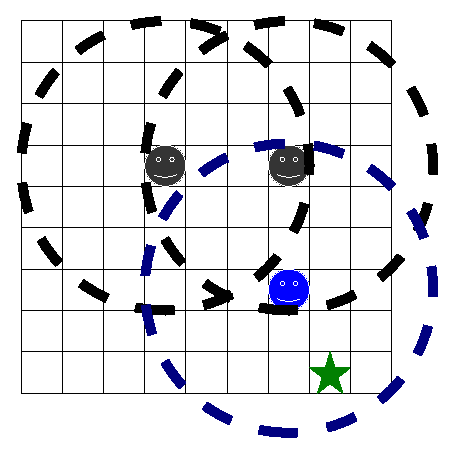
\includegraphics{reward_range.eps}
}
\caption[Schematische Darstellung der Rewardverteilung an ActionSets bei einem neutralen Ereignis] {Schematische Darstellung der Rewardverteilung an ActionSets bei einem neutralen Ereignis}
\label{reward_range:fig}
\end{figure}


\begin{figure}[htbp]
\centerline{	
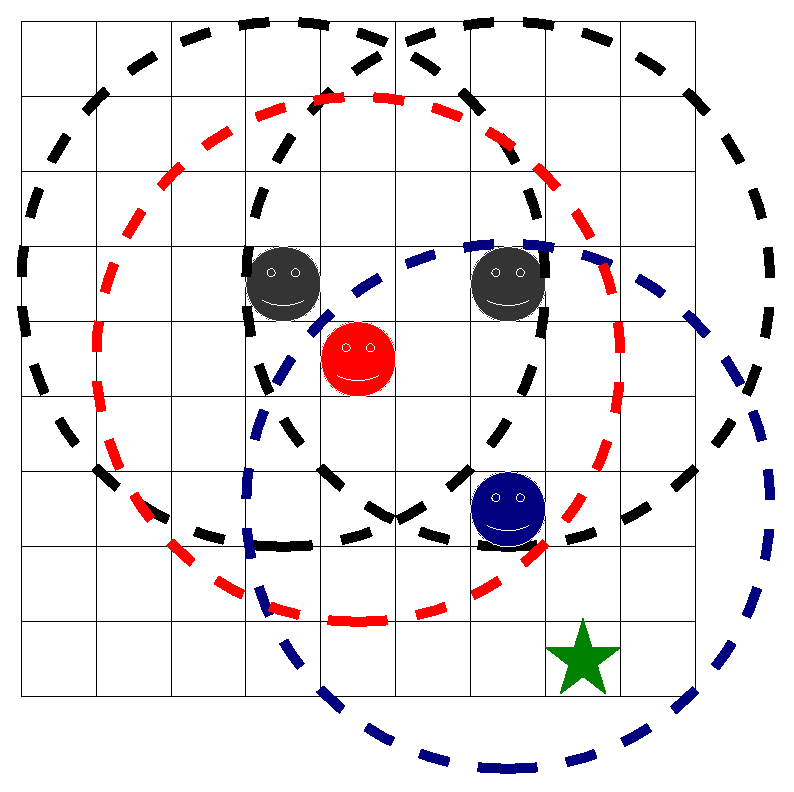
\includegraphics{reward_range_egoist.eps}
}
\caption[Schematische Darstellung der Rewardverteilung an ActionSets bei einem neutralen Ereignis] {Schematische Darstellung der Rewardverteilung an ActionSets bei einem neutralen Ereignis}
\label{reward_range_egoist:fig}
\end{figure}


\begin{figure}[htbp]
\centerline{	
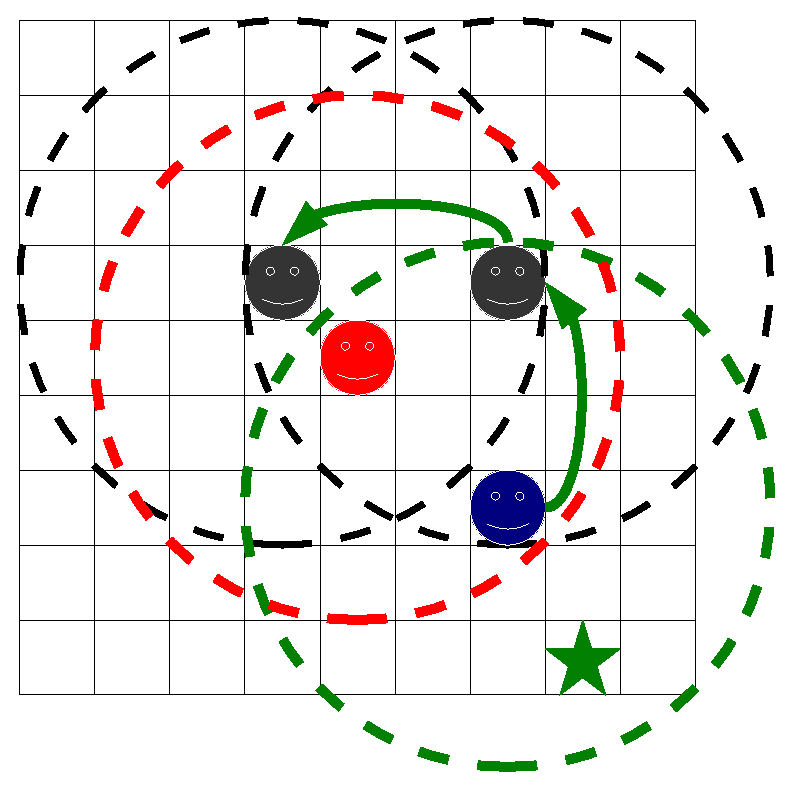
\includegraphics{reward_range_egoist_block.eps}
}
\caption[Schematische Darstellung der Rewardverteilung an ActionSets bei einem neutralen Ereignis] {Schematische Darstellung der Rewardverteilung an ActionSets bei einem neutralen Ereignis}
\label{reward_range_egoist_block:fig}
\end{figure}


\begin{program}
  \begin{verbatim}
    /**
     * Relation of this classifier set (the active agent classifier set,
     * e.g. the set that received a reward) to another classifier set
     * @param other The other set we want to compare with
     * @return degree of relationship (0.0 - 1.0)
     */
    public double checkEgoisticDegreeOfRelationship(
                    final MainClassifierSet other) {
        double ego_factor = 
                 getEgoisticFactor() - other.getEgoisticFactor();
        if(ego_factor == 0.0) {
            return 0.0;
        }
        return 1.0 - ego_factor * ego_factor;
    }

    public double getEgoisticFactor() throws Exception {
        double factor = 0.0;
        double pred_sum = 0.0;
        for(Classifier c : getClassifiers()) {
            if(!c.isPossibleSubsumer()) {
                continue;
            }
            factor += c.getEgoFactor();
            pred_sum += c.getFitness() * c.getPrediction();
        }
        if(pred_sum > 0.0) {
            factor /= pred_sum;
        } else {
            factor = 0.0;
        }
        return factor;
    }
\end{verbatim}
  \caption{``Egoistic relation'', Algorithmus zur Bestimmung des Kommunikationsfaktors basierend auf dem Verhalten des Agenten gegen�ber anderen Agenten}
\end{program}

\section{Realistischer Fall mit Kommunikationsrestriktionen}

Wann immer ein Reward an einen Agenten verteilt wird, kann es sinnvoll sein, diesen Reward an andere Agenten weiterzugeben. Bisher wurde der Fall betrachtet, dass Kommunikation mit beliebiger Reichweite stattfinden kann. Dies ist nat�rlich kein realistisches Szenario. Geht man jedoch davon aus, dass die Kommunikationsreichweite zumindest ausreichend gro� ist um nahe Agenten zu kontaktieren, so kann man argumentieren, dass man dadurch ein Kommunikationsnetzwerk aufbauen kann, in dem jeder Agent jeden anderen Agenten - mit einer gewissen Zeitverz�gerung - erreichen kann. Bei ausreichender Agentenzahl relativ zur freien Fl�che fallen dadurch nur vereinzelte Agenten aus dem Netz, was der Effektivit�t der Agentengruppe erwartungsgem�� nur geringf�gig schadet (TODO zeigen?)
Stehen die Agenten nicht indirekt andauernd miteinander in Kontakt (mit anderen Agenten als Proxy), sondern muss die Information zum Teil durch aktive Bewegungen der Agenten transportiert werden, tritt eine Zeitverz�gerung auf. Auch kann die ben�tigte Bandbreite die verf�gbare �bersteigen, was ebenfalls Zeit ben�tigt.
Im realistischen Fall ist also davon auszugehen, dass jede Kommunikation erst mit einer gewissen Verz�gerung ausgef�hrt wird, weshalb f�r Kommunikation nur der zuvor besprochene verz�gerte LCS Algorithmus in Frage kommt.

TODO lag einf�hren...

\section{Weitergabe des Rewards}

\section{Bewertung Kommunikation:}

Die Vorteile, die man durch Kommunikation erzielen kann, h�ngt stark durch das Szenario ab. Beispielsweise in dem Fall, bei dem zuf�llige Agenten bereits fast 100\% Abdeckung erreichen, also so viele Agenten auf dem Feld sind, dass der Gewinn durch Absprache minimal ist. Auch ist, weil wir nur mit Bin�rsensoren arbeiten, die Sensorik gest�rt, wenn sich sehr viele Agenten auf dem Feld befinden, weil die Sensoren sehr oft gesetzt sind und somit wenig Aussagekraft haben. Erweiterungen wie zus�tzliche Sensoren die die Abst�nde bestimmen w�rde hier wahrscheinlich klarere Ergebnisse liefern.
Umgekehrt ist der Einfluss bei sehr wenigen Agenten gering. TODO

Vergleich unterschiedliche Agentenanzahl, unterschiedliche Kommunikationsmittel
Vergleich mit LCS?

\subsection{Vergleich TODO}

Old LCS Agent
New LCS Agent

Multistep LCS Agent
Dieser Algorithmus stellt eine Implementation des Standard XCS Algorithmus dar. Unterschied zur Standardimplementation ist, dass die Probleminstanz bei Erreichen des tempor�ren Ziels (d.h. den Zielagenten in Sicht zu bekommen) nicht tats�chlich neugestartet wird.
Events, wie bei den neuen LCS Implementationen gibt es nicht, ist das Ziel in Sicht wird Reward 1.0 weitergegeben.

Single LCS Agent

Mehrere LCS Agenten (``Old LCS Agent'') teilen sich ein gemeinsames ClassifierSet, das sie entsprechend updaten.
Entspricht dem Extremfall der Kommunikation
Sight range/Kommunikationsrange





LCS Agenten schneiden auch ohne Kommunikation (bei ausreichender Anzahl von Schritten) immer besser ab als zuf�llige Agenten.

TODOGrafiken



\begin{figure}[htbp]
\centerline{	
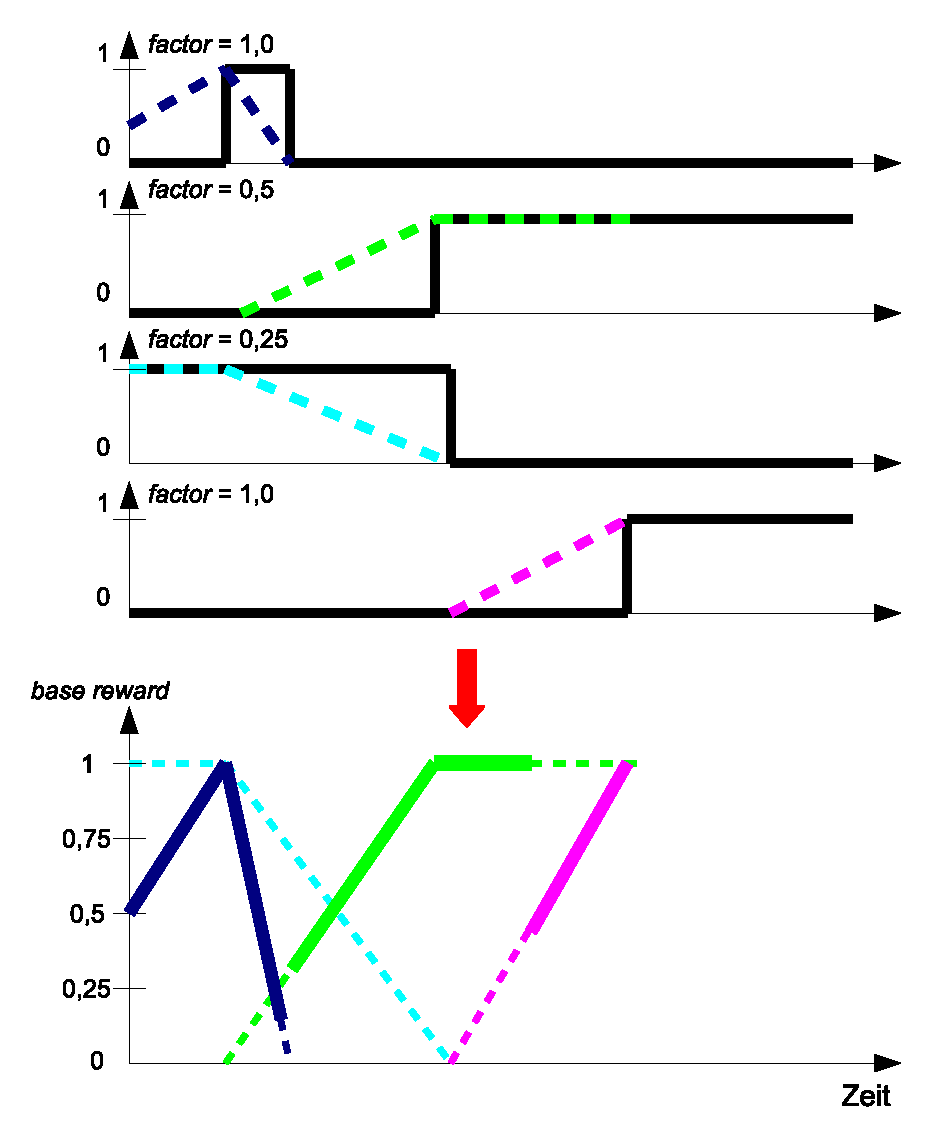
\includegraphics{corrected_reward.eps}
}
\caption[Beispielhafte Darstellung der Kombinierung interner und externer Rewards] {Beispielhafte Darstellung der Kombinierung interner und externer Rewards}
\label{corrected_reward:fig}
\end{figure}

\chapter{Zusammenfassung, Ergebnis und Ausblick}\label{conclusion:cha}


\section{Zusammenfassung}

Zu Beginn wurde auf die Szenariodefinition und die F�higkeiten der Agenten eingegangen. Anhand von Beispielen heuristischer Agenten wurden einige Grundeigenschaften der pr�sentierten Szenarien als Vorbereitung f�r die Analyse der Learning Classifier Systeme bestimmt. Nach der Einf�hrung in LCS, der Beschreibung des Standardverfahren XCS und der angepassten Implementierung f�r �berwachungsszenarios konnten dann umfangreiche Tests ausgef�hrt werden. 


von der M�glichkeit zur Kommunikation eine angepasste Implementierung f�r verz�gerten Reward definiert auf Basis dessen dann mehrere Varianten f�r die Weitergabe des Rewards vorgestellt, analysiert und verglichen wurden.

\section{Ergebnis}
Das wesentliche Ergebnis ist, dass die Implementierung des XCS auf  �berwachungsszenarios ausgeweitet werden kann ohne wesentliche Ver�nderungen am Algorithmus vorzunehmen. W�hrend sich die Qualit�t der resultierenden Agenten im Allgemeinen �ber dem zuf�lligen Agenten befindet, ist die Effizienz der Implementierung, im Vergleich zu einfachen Heuristiken, sehr gering. Mit der verwendeten Implementierung hat XCS Probleme, eine optimale Regelmenge zu finden bzw. zu halten. Eine Regel wie z.B. "`laufe auf das Ziel zu, wenn es in Sicht ist"', ist als Heuristik sehr erfolgreich, bei dauerhafter �berwachung ohne Kommunikation l�uft es aber eher auf ein Verfolgungsszenario hinaus. Aufgrund andauerndem Lernens TODO

Die alleinige Anpassung des XCS Multistepverfahrens, dass ein neues Problem gestartet wird, wann immer sich das Ziel in �berwachungsreichweite befand f�hrte nicht zum Erfolg, die Ergebnisse waren nicht besser als ein sich zuf�llig bewegender Agent.\\


Erst durch Verkn�pfung des Rewards mit dem zeitlichen Abstand zu einer �nderung des Zustands f�hrte zu deutlich besseren Ergebnissen.\\ TODO
Desweiteren wurde untersucht, inwiefern sich der Austausch an minimaler Information unter den Agenten, ohne zentrale Steuerung oder globalem Regeltausch, auf die Qualit�t auswirkt. Zwar gab es vereinzelt positive Effekte, diese waren jedoch auf andere Faktoren zur�ckzuf�hren.



empfindlich gegen�ber Parameter�nderungen

\section{Ausblick}
Ein 


Weitere Untersuchungen sind n�tig um zu bestimmen, inwiefern Kommunikation, beispielsweise mit einer gr��eren Zahl an besseren Sensoren, zu einem besseren Ergebnis f�hren kann. TODO\\
Vom theoretischen Standpunkt ist noch zu kl�ren, warum genau der zeitliche Abstand zum Erfolg gef�hrt hat und wo die Grenzen hierf�r liegen. 

Erschwerung, mehr Kollaboration
TODO aus verschiedenen Richtungen betrachten? Mehrere Agenten notwendig?

Probiert, aber verworfen:

W�hrend der Arbeit wurden auch einige Ans�tze probiert aber mangels Erfolgsaussichten wieder verworfen. Urspr�nglich wurde das Szenario auf Basis von Rotation konzipiert. Die Annahme war, dass ein Agent, der f�r einen Satz an Sensordaten eine optimales \emph{classifier set} gefunden hat, dieses \emph{classifier set} auch f�r Sensordaten eines um 90, 180 und 270 Grad gedrehten Szenarios (mit entsprechend 90, 180 und 270 Grad gedrehter Aktion des jeweiligen \emph{classifier}) optimal sei. Aufgrund der deutlichen Komplexit�tssteigerung des Programms, der niedrigeren Laufzeit und mangels konkreter Qualit�tssteigerungen gegen�ber dem Ansatz ohne Rotation wurde diese Idee jedoch fallengelassen. M�glicherweise k�nnte man durch Hinzunahme eines weiteren Bits im \emph{condition} Vektor, das bestimmt, ob dieser \emph{classifier} gleichzeitig auch die drei rotierten Szenarien erkennen kann, die Leistung des Systems verbessern, dies bedarf aber weiterer Untersuchung und geht am eigentlichen Thema dieser Arbeit vorbei.\\


Abnehmende Exploration LITERATUR
Intelligent Exploration Method to Adapt Exploration Rate in XCS, Based on Adaptive Fuzzy Genetic Algorithm
An Adaptive Approach for the Exploration-Exploitation Dilemma for Learning Agents 

Vielversprechend war anfangs eine Funktion mit der neuerstellte \emph{classifier} mit dem Durchschnittswert aller \emph{reward prediction} Werte einer \emph{classifier set} Liste initialisiert werden. Der Vorteil zeigte sich jedoch nur bei einer zu gering gew�hlten Populationsgr��e (unter 256, siehe Kapitel~\ref{sec:max_population_parameter}), also wenn andauernd neue \emph{classifier} durch \emph{covering} generiert werden m�ssen. Eine weitere Voraussetzung ist, dass sich die \emph{reward prediction} Werte �hneln. Im in dieser Arbeit untersuchten Fall, bei dem die Agenten nur begrenzte Sensorf�higkeiten besitzen, sich auf einem Torus frei bewegen k�nnen.

TODO!

dass sich die \emph{reward prediction} Werte der einzelnen \emph{classifier} untereinander wenig unterscheiden, w�hrend sie beispielsweise bei statischen Szenarien gegen feste, stark unterschiedliche Werte konvergieren. Beispielsweise im Einf�hrungsbeispiel in Abbildung~\ref{simple_scenario_multistep:fig} w�rden die \emph{reward prediction} Werte der \emph{classifier} b), c), e) und g) eher gegen 1 und die der restlichen \emph{classifier} gegen 0 streben.\\
Welchen Wert man f�r \(p_{i}\) nun als Durchschnittswert w�hlt, h�ngt vom jeweiligen Szenario ab. Beispielsweise w�rde ein �berwachungsszenario auf einem sehr gr��eren Torus mit relativ wenigen Agenten w�rde zu einem niedrigeren Durchschnittswert f�r die \emph{reward prediction} Variable f�hren und umgekehrt.\\


In Kapitel TODO wurde eine SXCS Variante vorgestellt, die sowohl mit der Weitergabe des \emph{maxPrediction} wie bei XCS als auch mit der direkten linearen bzw. quadratischen Weitergabe des \emph{base reward} Werts arbeitet. Dadurch ergeben sich Werte f�r den Maximalwert des \emph{reward} \(\rho\) (siehe Kapitel~\ref{epsilon0:sec}) gr��er \(1.0\), womit auch die \emph{reward prediction} Werte der \emph{classifier} aktualisiert werden, wodurch auch diese Werte wiederum gr��er werden, usw. Hier ist noch theoretische Arbeit zu leisten, wie logisch beide Arten der Weitergabe des \emph{reward} sinnvoll miteinander verkn�pft werden k�nnen. In dieser Arbeit konnte nur gezeigt werden, dass in bestimmten Szenarien diese Form der Weitergabe erfolgversprechend ist, wenn es auch f�r einen gewissen Grad der Verf�lschung (und somit auch einer niedrigeren Qualit�t) in Szenarien sorgt, die wenig auf das Erkennen von bestimmten Mustern (wie z.B. beim schwierigen Szenario die �ffnungen) ausgerichtet sind.\\



Sicher interessant ist auch der umgekehrte Ansatz, bei der das Zielobjekt das Objekt ist, das lernt, und den Agenten ausweichen muss. Dieser Aspekt konnte in der Arbeit nur kurz angesprochen werden.\\ TODO



Im Bereich der Kommunikation wurde neben in dieser Arbeit besprochenen "`egoistischen Relation"' (siehe Kapitel~\ref{egoistic_relation:sec}) auch weitere Verfahren ausprobiert, mit welchen versucht wurde, gleichartige Gruppen zu finden. Hier wurden ganze \emph{classifier set} Listen unterschiedlicher Agenten miteinander auf �hnlichkeit gepr�ft um daraus einen Faktor zu berechnen, der (wie bei der "`egoistischen Relation"') Einfluss auf die Weitergabe des \emph{reward} Werts haben sollte. Der dadurch deutlich erh�hte Kommunikations- und Berechnungsaufwand lag jedoch in keinem Verh�ltnis zu eventuell beobachteten Qualit�tsverbesserungen, im Gegenteil wurden eher Qualit�tsverschlechterungen beobachtet. Die Ergebnisse mit dem Test der "`egoistischen Relation"' zeigen jedoch, dass hier zumindest etwas Potential stecken k�nnte und f�r bestimmte Szenarien die zwei Grundideen, dass sich die Agenten zum einen an die Gr��e des Szenarios anpassen und zum anderen der \emph{reward} Wert m�glichst nur an sich �hnlich verhaltende Agenten weitergegeben wird, nicht ganz falsch sein k�nnen. Genauere, insbesondere theoretische, Untersuchungen sind hier n�tig.\\



Was die Szenarien selbst betrifft, wurden ebenfalls mehrere verworfen, da bei ihnen keine zus�tzlichen Beobachtungen gemacht bzw. nur unbedeutende Teilaspekte betrachtet werden konnten. Unter anderem sind dies ein Labyrinth, dessen Umsetzung wahrscheinlich an den mangelnden F�higkeiten der Sensoren scheiterte, ein vereinfachtes "`schwieriges Szenario"' mit einem "`Raum"' mit einer �ffnung in der Mitte, welches sich als zu einfach zu l�sen herausstellte und ein Szenario mit einem Kreuz bestehend aus Hindernissen in der Mitte, welches keine bedeutend anderen Ergebnisse lieferte als das Szenario mit zuf�llig verteilten Hindernissen.\\



\section{Vorgehen und verwendete Hilfsmittel und Software}

Zu Beginn stellte sich die Frage, welche Software zu benutzen ist, da es sich um ein recht komplexe Problemstellung handelt. Begonnen wurde mit der YCS~Implementierung~\cite{Bull03asimple}. Sie ist in der Literatur wenig vertreten, die Implementierung bot aber einen guten Einstieg in das Thema, da sie sich auf das Wesentliche eines LCS beschr�nkte und nur wenige Optimierungen enthielt.\\
Auf Basis des dadurch gewonnenen Wissens war es dann leichter, die XCS Implementierung zu verstehen und nachvollziehen zu k�nnen. Insbesondere die Optimierungen und der etwas unsaubere Programmierstil in der Standardimplementierung bereiteten Probleme.\\

Anhand des Studiums der Literatur war klar, dass in der Richtung der �berwachungsszenarien es wenig Arbeiten, die sich damit besch�ftigten, wie die XCS Implementierung umzusetzen sei. Ein R�ckgriff auf bestehende Bibliotheken war deshalb nicht m�glich, urspr�nglich geplante Untersuchungen komplexerer Systeme wie zentrale Steuerung, Austausch von Regeln etc. wurden gestrichen und es wurde sich auf den einfachen Fall, lokale Information ohne zentrale Steuerung mit h�chstens minimaler Kommunikation beschr�nkt. Dies machte die Verwendung komplexerer Simulationssysteme unn�tig, die Einarbeitungszeit in Multiagenten Frameworks wie z.B. Repast~\cite{repast} erschien zu hoch, wie auch die Risiken, was Geschwindigkeit, Kompatibilit�t und Speicherverbrauch betraf, unbekannt waren, weshalb ein eigenes Simulationsprogramm entwickelt wurde.\\

Das Simulationsprogramm samt zugeh�riger Oberfl�che~\cite{agentsimulator} zur Erstellung von neuen Test-Jobs wurde in Java mit Hilfe von NetBeans~IDE~6.5~\cite{NetBeans} selbst entwickelt und gestaltet.\\

F�r die Verlaufsgraphen wurde GnuPlot~4.2.4~\cite{GnuPlot} benutzt, die Darstellungen der jeweiligen Konfiguration des Torus (insbesondere in Kapitel~\ref{scenario_description:cha}) wurden im Programm mittels Gif89Encoder~\cite{gifencoder} erstellt. Weitere Graphen und Darstellungen wurden OpenOffice.org~Impress und OpenOffice.org~Calc~\cite{OpenOffice} erstellt.\\
Wesentlicher Bestandteil der Konfigurationsoberfl�che war auch eine Automatisierung der Erstellung von Konfigurationsdateien und Batchdateien f�r ein Einzelsystem bzw. f�r JoSchKA~\cite{JoSchKa} zum Testen einer ganzen Reihe von Szenarien und GnuPlot Skripts. Die Automatisierung war aufgrund der tausenden getesteten Szenarien und Parametereinstellungen entscheidend zur Durchf�hrung dieser Arbeit.\\
Dieses Dokument schlie�lich wurde mittels dem \LaTeX Editor LEd 0.5263 \cite{LeD} erstellt und mittels MiKTeX~2.7~\cite{miktex} kompiliert.



\section{Beschreibung des Konfigurationsprogramms}

\begin{figure}[htbp]
\centerline{	
%\includegraphics{agent_configuration.eps}
}
\caption[Screenshot des Konfigurationsprogramms] {Screenshot des Konfigurationsprogramms}
\label{agent_configuration:fig}
\end{figure}





\begin{appendix}
\chapter{Implementation}\label{implementation:cha}

\section{Implementierung eines Problemablaufs}\label{implementierung_ablauf:sec}

In der Schleife der Funktion zur Berechnung eines Experiments (Programm~\ref{mainExperiment:pro}) wird die Funktion zur Berechnung des Problems (\emph{doOneMultiStepProblem()} in Programm~\ref{mainProblem:pro}) aufgerufen. Dort wird in einer weiteren Schleife �ber die Anzahl der maximalen Schritte die Sicht aktualisiert (\emph{updateSight()}), die Qualit�t bestimmt (\emph{updateStatistics()}), die neuen Sensordaten und die n�chste Aktion ermittelt (\emph{calculateAgents()}, siehe Programm~\ref{mainCalculate:pro}), der \emph{reward} Wert ermittelt (\emph{rewardAgents()}, siehe Programm~\ref{mainReward:pro}) und schlie�lich werden die Objekte bewegt (\emph{moveAgents()}, siehe Programm~\ref{mainMove:pro}). Die konkrete Umsetzung der dort aufgerufenen Funktionen (insbesondere \emph{calculateNextMove()} und \emph{calculateReward()}) wird im Kapitel~\ref{lcs_variants:cha} erl�utert (bzw. in Kapitel~\ref{agents:cha}, was die Heuristiken betrifft, wobei \emph{calculateReward()} dort keine Rolle spielt und eine leere Funktion aufgerufen wird).

\newlisting{Zentrale Schleife f�r einzelne Experimente}{mainExperiment:pro}
/**
 * F�hrt eine Anzahl von Problemen aus
 * @param experiment_nr Nummer des auszuf�hrenden Experiments
 */
  public void doOneMultiStepExperiment(int experiment_nr) {
    int currentTimestep = 0;

  /**
   * number of problems for the same population
   */
    for (int i = 0; i < Configuration.getNumberOfProblems(); i++) {

    /**
     * Initialisierung des neuen "Random Seed" Wert
     */
      Misc.initSeed(Configuration.getRandomSeed() + 
        experiment_nr * Configuration.getNumberOfProblems() + i);

    /**
     * Erstellt einen neuen Torus und verteilt Agenten und 
     *   das Zielobjekt neu
     */
      BaseAgent.grid.resetState();

    /**
     * F�hre Problem aus und aktualisiere aktuellen Zeitschritt
     */
      currentTimestep = doOneMultiStepProblem(currentTimestep);
    }
  }
\end{lstlisting}

\newlisting{Zentrale Schleife f�r einzelne Probleme}{mainProblem:pro}
/**
 * F�hrt eine Anzahl von Schritten auf dem aktuellen Torus aus
 * @param stepCounter Aktuelle Zeitschritt
 * @return Der Zeitschritt nach der Ausf�hrung
 */
  private int doOneMultiStepProblem(int stepCounter) {
  /**
   * Zeitpunkt bis zu dem das Problem ausgef�hrt wird
   */
    int steps_next_problem = 
      Configuration.getNumberOfSteps() + stepCounter;    
    for (int currentTimestep = stepCounter; 
         currentTimestep < steps_next_problem; currentTimestep++) {

    /**
     * Ermittle die Sichtbarkeit und erhebe Statistiken
     */
      BaseAgent.grid.updateSight();
      BaseAgent.grid.updateStatistics(currentTimestep);

    /**
     * Ermittle neue Sensordaten und berechne Aktionen der Agenten
     */
      calculateAgents(currentTimestep);

    /**
     * Ermittle den Reward f�r alle Agenten (nach dem ersten Schritt)
     */
      if(currentTimestep > stepCounter) {
        rewardAgents(currentTimestep);
      }

    /**
     * F�hre zuvor berechnete Aktionen aus
     */
      moveAgents();
    }

    /**
     * Abschlie�ende Ermittlung des Rewards
     */
    BaseAgent.grid.updateSight();
    rewardAgents(steps_next_problem);
    return steps_next_problem;
  }
\end{lstlisting}





\newlisting{Zentrale Bearbeitung (Sensordaten und Berechnung der neuen Aktion) aller Agenten und des Zielobjekts innerhalb eines Problems}{mainCalculate:pro}
/**
 * Berechnet die Aktionen und f�hrt sie in zuf�lliger Reihenfolge aus
 * @param gaTimestep der aktuelle Zeitschritt
 */
  private void calculateAgents(final long gaTimestep) {

  /**
   * Ermittle Sensordaten und bestimme n�chste Bewegung
   */
    for(BaseAgent a : agentList) {
      a.aquireNewSensorData();
      a.calculateNextMove(gaTimestep);
    }
    BaseAgent.goalAgent.aquireNewSensorData();
    BaseAgent.goalAgent.calculateNextMove(gaTimestep);
  }
\end{lstlisting}



\newlisting{Zentrale Bearbeitung (Verteilung des \emph{reward} Werts) aller Agenten und des Zielobjekts innerhalb eines Problems}{mainReward:pro}
/**
 * Verteilt den Reward an alle Agenten
 */
  private void rewardAgents(final long gaTimestep) {
    for(BaseAgent a : agentList) {
      a.calculateReward(gaTimestep);
    }
    BaseAgent.goalAgent.calculateReward(gaTimestep);
  }
\end{lstlisting}



\newlisting{Zentrale Bearbeitung (Ausf�hrung der Bewegung) aller Agenten und des Zielobjekts innerhalb eines Problems}{mainMove:pro}
/**
 * Berechnet die Aktionen und f�hrt sie in zuf�lliger Reihenfolge aus
 * @param gaTimestep der aktuelle Zeitschritt
 */
  private void moveAgents(long gaTimestep) {
  /**
   * Erstelle Ausf�hrungsliste f�r alle Objekte (Zielobjekt mehrfach)
   */
    int goal_speed = Configuration.getGoalAgentMovementSpeed();
    ArrayList<BaseAgent> random_list = 
      new ArrayList<BaseAgent>(agentList.size() + goal_speed);

    random_list.addAll(agentList);
    for(int i = 0; i < goal_speed; i++) {
      random_list.add(BaseAgent.goalAgent);
    }

  /**
   * F�hre die ermittelten Aktionen in zuf�lliger Reihenfolge aus
   *   (Zielobjekt kann mehrfach ausgef�hrt werden).
   */
    int[] array = Misc.getRandomArray(random_list.size());
    for(int i = 0; i < array.length; i++) {
      BaseAgent a = random_list.get(array[i]);
      a.doNextMove();
      if(a.isGoalAgent() && goal_speed > 1) {
        goal_speed--;
        a.aquireNewSensorData();
        a.calculateNextMove(gaTimestep);
        a.calculateReward(gaTimestep);
      }
    }
  }
\end{lstlisting}

\clearpage



\section{Typen von Agentenbewegungen}

\newlisting{Berechnung der n�chsten Aktion bei der Benutzung des Algorithmus mit zuf�lliger Bewegung}{calculateNextMoveRandomAlgorithm:pro}
/**
 * Berechne n�chste Aktion (zuf�lliger Algorithmus)
 */
  private void calculateNextMove() {
  /**
   * W�hle zuf�llige Richtung als n�chste Aktion
   */
    calculatedAction = Misc.nextInt(Action.MAX_DIRECTIONS);
  }
\end{lstlisting}


\newlisting{Berechnung der n�chsten Aktion bei der Benutzung der einfachen Heuristik}{calculateNextMove_SimpleHeuristic:pro}
/**
 * Berechne n�chste Aktion (einfache Heuristik)
 */
  private void calculateNextMove() {
  /**
   * Holt sich die Informationen der Gruppe der Sensoren, die auf 
   * das Zielobjekt ausgerichtet sind
   */
    boolean[] goal_sensor = lastState.getSensorGoal();
    calculatedAction = -1;
    for(int i = 0; i < Action.MAX_DIRECTIONS; i++) {
    /**
     * Zielagent in Sicht in dieser Richtung?
     */
      if(goal_sensor[2*i]) {
        calculatedAction = i;
        break;
      }
    }

  /**
   * Sonst w�hle zuf�llige Richtung als n�chste Aktion
   */
    if(calculatedAction == -1) {
      calculatedAction = Misc.nextInt(Action.MAX_DIRECTIONS);
    }      

  }
\end{lstlisting}

\newlisting{Berechnung der n�chsten Aktion bei der Benutzung der intelligenten Heuristik}{calculateNextMove_IntelligentHeuristic:pro}
/**
 * Berechne n�chste Aktion (intelligente Heuristik)
 */
private void calculateNextMove() {
  /**
   * Holt sich die Informationen der Gruppe der Sensoren, die auf 
   * das Zielobjekt ausgerichtet sind
   */
    boolean[] goal_sensor = lastState.getSensorGoal();

    calculatedAction = -1;
    for(int i = 0; i < Action.MAX_DIRECTIONS; i++) {
    /**
     * Zielagent in Sicht in dieser Richtung?
     */
      if(goal_sensor[2*i]) {
        calculatedAction = i;
        break;
      }
    }

  /**
   * Zielobjekt nicht in Sicht? Dann bewege von Agenten weg
   */
    if(calculatedAction == -1) {
      calculatedAction = Misc.nextInt(Action.MAX_DIRECTIONS);

      boolean[] agent_sensors = lastState.getSensorAgent();
      boolean one_free = false;
      for(int i = 0; i < Action.MAX_DIRECTIONS; i++) {
        if(!agent_sensors[2*i]) {
          one_free = true;
          break;
        }
      }

      if(one_free) {
        while(agent_sensors[2*calculatedAction]) {
          calculatedAction = Misc.nextInt(Action.MAX_DIRECTIONS);
        }
      }
    } 
  }
\end{lstlisting}

\clearpage



\section{Korrigierte \emph{addNumerosity()} Funktion}\label{corrected_numerosity_function:sec}

Durch die Benutzung von \emph{macro classifier} ergibt sich das programmiertechnische Problem, dass man nicht mehr direkt wei�, wieviele \emph{micro classifier} sich in einer Population befinden, bei jeder Benutzung des Werts der Populationsgr��e m�ssten die \emph{numerosity} Werte aller \emph{classifier} jedes Mal addiert werden. In der Standardimplementierung \cite{Butz_xcsclassifier} ist die Behandlung des \emph{numerosity} Werts deswegen stark optimiert, jedes \emph{classifier set} tr�gt eine tempor�re Variable \emph{numerositySum} mit sich, in der die aktuelle Summe gespeichert ist. Die Aktualisierung ist jedoch zum einen mangelhaft umgesetzt, zum anderen auf die Verwendung von einer einzelnen \emph{action set} Liste optimiert, w�hrend die hier verwendete Implementierung jeweils mit bis �ber 100 \emph{action set} Listen programmiert wurde, denen ein \emph{classifier} Mitglied sein kann. Deswegen wurde die Optimierung entfernt und durch eine dezentrale Verwaltung mit einem \emph{Observer} ersetzt, jede �nderung des \emph{numerosity} Wertes hat also die �nderung aller \emph{action set} Listen zur Folge, in der der \emph{classifier} Mitglied ist.\\

Wird also z.B. ein \emph{micro classifier} entfernt, dann wird lediglich die �nderungsfunktion des \emph{classifiers} aufgerufen, der dann wiederum den \emph{numerositySum} Wert der jeweiligen Eltern anpasst. Dies macht einige Optimierungen r�ckg�ngig, erspart aber sehr viel Umst�nde, den \emph{numerositySum} der Eltern immer auf den aktuellen Stand zu halten und einzelne \emph{classifiers} zu l�schen.\\

Positiver Nebeneffekt durch die verbesserte Struktur ist, dass man dadurch leicht auf die Menge der \emph{action set} Listen zugreifen kann, denen ein \emph{classifier} angeh�rt, hierf�r wurde aber im Rahmen dieser Arbeit keine Verwendung gefunden.\\

Ein weiteres Problem der Standardimplementierung ist, dass der \emph{fitness} Wert eines \emph{classifiers} als Optimierung bereits den \emph{numerosity} Wert als Faktor enth�lt, w�hrend bei der Aktualisierung des \emph{numerosity} Werts der \emph{fitness} Wert nicht aktualisiert wurde. Das hat zur Folge, dass theoretisch \emph{fitness} Werte von \emph{classifiers} fast den \emph{max population} Wert annehmen kann, wenn ein \emph{classifier} mit \emph{numerosity} und \emph{fitness} Wert in der H�he von \emph{max population} auf einen \emph{numerosity} Wert von \(1,0\) reduziert wird.\\
Dies betrifft die Funktion \emph{public void addNumerosity(int num)} der Klasse \emph{XClassifier} in der Datei \emph{XClassifier.java}. Die Korrektur besteht darin, den \emph{fitness} Wert mit dem Quotienten aus dem neuen durch den alten \emph{numerosity} Wert zu multiplizieren. Die korrigierte Fassung ist in Programm~\ref{corrected_numerosity_function:pro} dargestellt.\\

M�glicherweise kann man diesen Fehler durch Ver�nderung der Parameter oder l�ngere Laufzeiten kompensieren, logisch betrachtet macht es aber keinen Sinn, dass beim Subsummieren bzw. L�schen eines \emph{micro classifier} der \emph{fitness} Wert ver�ndert wird. In Tests haben sich nur minimale Unterschiede ergeben. Beispielsweise ergab sich (auf dem S�ulenszenario mit 8 Agenten mit SXCS und einem Zielobjekt mit einfacher Richtungs�nderung) eine Qualit�t von \(39,15\%\) im Vergleich zur originalen Implementierung von \(39,95\%\) bei 500 Schritten bzw. \(35,42\%\) zu \(35,01\%\) bei 2000 Schritten. Der Fehler scheint sich also eher langfristig auszuwirken, wenn auch der Unterschied so klein ist, dass man ihn vernachl�ssigen kann. Problematisch wird es, wenn Modifikationen von XCS darauf aufbauen, dass der \emph{fitness} Wert f�r jeden \emph{micro classifier} immer kleiner gleich \emph{1.0} ist.\\

Alles in allem betrachtet soll im Rahmen dieser Arbeit soll die korrigierte Fassung benutzt werden.

\newlisting{Korrigierte Version der \emph{addNumerosity()} Funktion}{corrected_numerosity_function:pro}
/**
 * Erh�ht oder erniedrigt den numerosity Wert des classifier
 * @param num Der zur numerosity zu addierende Wert (kann negativ sein).
 */
  public void addNumerosity(int num) {
    int old_num = numerosity;
   
    numerosity += num;

  /**
   * Korrektur der fitness
   */
    if(old_num > 0) {
      fitness = fitness * (double)numerosity / (double)old_num;
    } else {
      fitness = Configuration.
    }

  /**
   * Aktualisierung der Eltern
   */
    for (ClassifierSet p : parents) {
      p.changeNumerositySum(num);
      if (numerosity == 0) {
        p.removeClassifier(this);
      }
    }
  }
\end{lstlisting}


\clearpage

\section{Implementierung XCS Multistepverfahrens }

\newlisting{Erstes Kernst�ck des Standard XCS Multistepverfahrens (\emph{calculateReward()}, Bestimmung und Verarbeitung des \emph{reward} Werts anhand der Sensordaten), angepasst an ein dynamisches �berwachungsszenario, bei positivem \emph{reward} Wert wird nicht abgebrochen}{multistep_calc_reward:pro}
/**
 * Diese Funktion wird in jedem Schritt aufgerufen um den aktuellen
 * reward zu bestimmen, den besten Wert der ermittelten match set Liste
 * weiterzugeben und, bei aktuell positivem reward, die aktuelle
 * action set Liste zu belohnen.
 *
 * @param gaTimestep Der aktuelle Zeitschritt
 */

  public void calculateReward(final long gaTimestep) {
  /**
   * checkRewardPoints liefert "wahr" wenn sich das Zielobjekt in
   * �berwachungsreichweite befindet
   */
    boolean reward = checkRewardPoints();

    if(prevActionSet != null){
      collectReward(lastReward, lastMatchSet.getBestValue(), false);
      prevActionSet.evolutionaryAlgorithm(classifierSet, gaTimestep);
    }

    if(reward) {
      collectReward(reward, 0.0, true);
      lastActionSet.evolutionaryAlgorithm(classifierSet, gaTimestep);
      prevActionSet = null;
      return;
    }
    prevActionSet = lastActionSet;
    lastReward = reward;
  }
\end{lstlisting}


\newlisting{Zweites Kernst�ck des XCS \emph{multi step} Verfahrens (\emph{collectReward()} - Verteilung des \emph{reward} Werts auf die \emph{action set} Listen), angepasst an ein dynamisches �berwachungsszenario}{multistep_collect_reward:pro}
/**
 * Diese Funktion verarbeitet den �bergebenen reward Wert und 
 * gibt ihn an die zugeh�rigen action set Listen weiter.
 *
 * @param reward Wahr wenn das Zielobjekt in Sicht war.
 * @param best_value Bester Wert des vorangegangenen action set Listen
 * @param is_event Wahr wenn diese Funktion wegen eines Ereignisses, 
 *          d.h. einem positiven reward Wert, aufgerufen wurde
 */

  public void collectReward(boolean reward, 
                double best_value, boolean is_event) {
    double corrected_reward = reward ? 1.0 : 0.0;

  /**
   * Falls der reward Wert von einem Ereignis r�hrt, aktualisiere die 
   * aktuelle action set Liste und l�sche das vorherige
   */
    if(is_event) {
      if(lastActionSet != null) {
        lastActionSet.updateReward(corrected_reward, best_value, factor);
        prevActionSet = null;
      }
    } 

  /**
   * Kein Ereignis, also nur die letzte action set Liste aktualisieren
   */
    else 
    {
      if(prevActionSet != null) {
        prevActionSet.updateReward(corrected_reward, best_value, factor);
      }
    }
  }
\end{lstlisting}



\newlisting{Drittes Kernst�ck des XCS \emph{multi step} Verfahrens (\emph{calculateNextMove()}, Auswahl der n�chsten Aktion und Ermittlung der zugeh�rigen \emph{action set} Liste), angepasst an ein dynamisches �berwachungsszenario}{multistep_calc_move:pro}
/**
 * Bestimmt die zum letzten bekannten Status passenden classifier und
 * w�hlt aus dieser Menge eine Aktion. Au�erdem wird die aktuelle 
 * action set Liste mithilfe der gew�hlten Aktion ermittelt.
 *
 * @param gaTimestep Der aktuelle Zeitschritt
 */

  public void calculateNextMove(long gaTimestep) {

 /**
  * �berdecke das classifierSet mit zum Status passenden Classifiern
  * welche insgesamt alle m�glichen Aktionen abdecken.
  */
    classifierSet.coverAllValidActions(
                    lastState, getPosition(), gaTimestep);

 /**
  * Bestimme alle zum Status passenden Classifier.
  */
    lastMatchSet = new AppliedClassifierSet(lastState, classifierSet);

 /**
  * Entscheide auf welche Weise die Aktion ausgew�hlt werden soll.
  */
    lastExplore = checkIfExplore(lastState.getSensorGoalAgent(),
                                           lastExplore, gaTimestep);

 /**
  * W�hle Aktion und bestimme zugeh�rige action set Liste
  */
    calculatedAction = lastMatchSet.chooseAbsoluteDirection(lastExplore);
    lastActionSet = new ActionClassifierSet(lastState, lastMatchSet,
                                                      calculatedAction);
  }
\end{lstlisting}



\clearpage

\section{Implementierung des SXCS Verfahrens}

\newlisting{Erstes Kernst�ck des SXCS-Algorithmus (\emph{calculateReward()}, Bestimmung des Rewards anhand der Sensordaten)}{sxcs_calc_reward:pro}
/**
 * Diese Funktion wird in jedem Schritt aufgerufen um den aktuellen
 * reward Wert zu bestimmen und positive, negative und neutrale 
 * Ereignisse den besten Wert der ermittelten match set Liste 
 * weiterzugeben und, bei aktuell positivem reward Wert, die 
 * aktuelle action set Liste zu belohnen.
 *
 * @param gaTimestep Der aktuelle Zeitschritt
 */

  public void calculateReward(final long gaTimestep) {
  /**
   * checkRewardPoints liefert "wahr" wenn sich der Zielobjekt in
   * �berwachungsreichweite befindet
   */
    boolean reward = checkRewardPoints();

    if (reward != lastReward) {
      int start_index = historicActionSet.size() - 1;
      collectReward(start_index, actionSetSize, reward, 1.0, true);
      actionSetSize = 0;
    }
    else 

    if(actionSetSize >= Configuration.getMaxStackSize())
    {
      int start_index = Configuration.getMaxStackSize() / 2;
      int length = actionSetSize - start_index;
      collectReward(start_index, length, reward, 1.0, false);
      actionSetSize = start_index;
    }

    lastReward = reward;
  }
\end{lstlisting}




\newlisting{Zweites Kernst�ck des SXCS-Algorithmus (\emph{collectReward()} - Verteilung des \emph{reward} Werts auf die \emph{action set} Listen)}{sxcs_collect_reward:pro}
/**
 * Diese Funktion verarbeitet den �bergebenen reward und gibt ihn an 
 * die zugeh�rigen action set Listen weiter.
 *
 * @param reward Wahr wenn der Zielobjekt in Sicht war.
 * @param best_value Bester Wert des vorangegangenen action set Listen
 * @param is_event Wahr wenn diese Funktion wegen eines Ereignisses, 
 *          d.h. einem positiven reward Wert, aufgerufen wurde
 */

  public void collectReward(int start_index, int action_set_size, 
                boolean reward, double best_value, boolean is_event) {
    double corrected_reward = reward ? 1.0 : 0.0;
  /**
   * Keine Weitergabe des reward Werts wie bei XCS
   */
    double max_prediction = 0.0;

  /**
   * Aktualisiere eine ganze Anzahl von action set Listen
   */
    for(int i = 0; i < action_set_size; i++) {

  /**
   * Benutze aufsteigenden bzw. absteigenden reward Wert bei einem 
   * positiven bzw. negativen Ereignis
   */
      if(is_event) {
        corrected_reward = reward ? 
          calculateReward(i, action_set_size) : 
          calculateReward(action_set_size - i, 
action_set_size);
      }
  /**
   * Aktualisiere die action set Liste mit dem bestimmten reward Wert 
   * und gebe bei allen anderen action set Listen den reward Wert 
   * weiter wie beim multi step Verfahren 
   */
      ActionClassifierSet action_classifier_set = 
        historicActionSet.get(start_index - i);
      action_classifier_set.updateReward(
        corrected_reward, max_prediction, factor);
    }
  }
\end{lstlisting}



\newlisting{Drittes Kernst�ck des SXCS-Algorithmus (\emph{calculateNextMove()} - Auswahl der n�chsten Aktion und Ermittlung und Speicherung der zugeh�rigen \emph{action set} Liste)}{sxcs_calc_move:pro}
/**
 * Bestimmt die zum letzten bekannten Status passenden classifier und
 * w�hlt aus dieser Menge eine Aktion. Au�erdem wird die aktuelle 
 * action set Liste mithilfe der gew�hlten Aktion ermittelt.
 * Im Vergleich zum originalen multi step Verfahren wird am Schluss noch 
 * die ermittelte action set Liste gespeichert.
 *
 * @param gaTimestep Der aktuelle Zeitschritt
 */

  public void calculateNextMove(long gaTimestep) {

 /**
  * �berdecke das classifierSet mit zum Status passenden Classifiern
  * welche insgesamt alle m�glichen Aktionen abdecken.
  */
    classifierSet.coverAllValidActions(
                    lastState, getPosition(), gaTimestep);

 /**
  * Bestimme alle zum Status passenden classifier.
  */
    lastMatchSet = new AppliedClassifierSet(lastState, classifierSet);

 /**
  * Entscheide auf welche Weise die Aktion ausgew�hlt werden soll,
  * w�hle Aktion und bestimme zugeh�riges action set Liste
  */
    lastExplore = checkIfExplore(lastState.getSensorGoalAgent(),
                                           lastExplore, gaTimestep);

    calculatedAction = lastMatchSet.chooseAbsoluteDirection(lastExplore);
    lastActionSet = new ActionClassifierSet(lastState, lastMatchSet,
                                                      calculatedAction);

 /**
  * Speichere die action set Liste, erh�he die Gr��e des Stacks und
  * und passe den Stack bei einem �berlauf an
  */
    actionSetSize++;
    historicActionSet.addLast(lastActionSet);
    if (historicActionSet.size() > Configuration.getMaxStackSize()) {
      historicActionSet.removeFirst();
    }
  }
\end{lstlisting}

\clearpage


\section{Implementation des DSXCS Algorithmus}

\newlisting{Zweites Kernst�ck des verz�gerten SXCS Algorithmus DSXCS (\emph{collectReward()} - Bewertung der \emph{action set} Listen)}{collect_reward_dsxcs:pro}
/**
 * Diese Funktion verarbeitet den �bergebenen reward Wert und gibt ihn an 
 * die zugeh�rigen action set Listen weiter. Wesentlicher Unterschied zum 
 * SXCS Algorithmus ist, dass der maxPrediction Wert erst bei der 
 * endg�ltigen Verarbeitung des historicActionSet Listen ermittelt wird.
 *
 * @param reward Wahr wenn das Zielobjekt in Sicht war.
 * @param best_value Bester Wert des vorangegangenen action set Listen
 * @param is_event Wahr wenn diese Funktion wegen eines Ereignisses, 
 *          d.h. einem positiven reward Wert, aufgerufen wurde
 */

  public void collectReward(int start_index, int action_set_size, 
                boolean reward, double best_value, boolean is_event) {
    double corrected_reward = reward ? 1.0 : 0.0;

  /**
   * Aktualisiere eine ganze Anzahl von Eintr�gen im historicActionSet
   */
     for(int i = 0; i < action_set_size; i++) {

  /**
   * Benutze aufsteigenden bzw. absteigenden reward Wert bei 
   * einem positiven bzw. negativen Ereignis
   */
       if(is_event) {
         corrected_reward = reward ? 
           calculateReward(i, action_set_size) : 
           calculateReward(action_set_size - i, action_set_size);
       } else {
         if(corrected_reward == 1.0 && factor == 1.0) {
           historicActionSet.get(start_index - i).
             rewardPrematurely(
               historicActionSet.get(start_index - i + 1).getBestValue());
         }
       }

  /**
   * F�ge den ermittelten reward Wert zum historicActionSet
   */
       historicActionSet.get(start_index - i).
         addReward(corrected_reward, factor);

    }
  }
\end{lstlisting}


\newlisting{Auszug aus dem dritten Kernst�ck des verz�gerten SXCS Algorithmus DSXCS (\emph{calculateNextMove()})}{dsxcs_calc_move:pro}

/**
 * Der erste Teil der Funktion ist identisch mit der calculateNextMove()
 * Funktion der SXCS Variante ohne Kommunikation. Der Zusatz ist, dass beim 
 * �berlauf die in der historicActionSet Liste gespeicherte reward Werte
 * verarbeitet werden
 */

  public void calculateNextMove(long gaTimestep) {
 
  // ... 

  /**
   * historyActionSet voll? Dann verarbeite den dort gespeicherten 
   * reward Wert
   */
     if (historicActionSet.size() > Configuration.getMaxStackSize()) {
      HistoryActionClassifierSet first = historicActionSet.pop();
      last.processReward(historicActionSet.getFirst().getBestValue());
    }
  }
\end{lstlisting}


\newlisting{Viertes Kernst�ck des verz�gerten SXCS Algorithmus DSXCS  (Verarbeitung des jeweiligen reward Werts, \emph{processReward()})}{process_reward_dsxcs1:pro}
/**
 * Zentrale Routine des HistoryActionSets zur Verarbeitung aller 
 * eingegangenen Rewards bis zu diesem Punkt.
 */

  public void processReward(double max_prediction) {

  /**
   * Finde das gr��te reward / factor Paar TODO Verbessern
   */
    for(RewardHelper r : reward) {
    /**
     * Dieser Eintrag wurde schon in collectReward() verwertet
     */
      if(r.reward == 1.0 && r.factor == 1.0) {
        continue;
      }
    /**
     * Aktualisiere den Eintrag mit den entsprechenden Werten und dem
     * �bergebenen maxPrediction Wert
     */
      actionClassifierSet.updateReward(r.reward, max_prediction, r.factor);
    }
  }
\end{lstlisting}


\newlisting{Verbesserte Variante des vierten Kernst�ck des verz�gerten SXCS Algorithmus DSXCS (Verarbeitung des reward Werts, \emph{processReward()})}{process_reward_dsxcs2:pro}
/**
 * Zentrale Routine des HistoryActionSets zur Verarbeitung aller 
 * eingegangenen Rewards bis zu diesem Punkt.
 */

  public void processReward(double max_prediction) {

    double max_value = 0.0;
    double max_reward = 0.0;
  /**
   * Finde das gr��te reward / factor Paar TODO Verbessern
   */
    for(RewardHelper r : reward) {
    /**
     * Dieser Eintrag wurde schon in collectReward() verwertet
     */
      if(r.reward == 1.0 && r.factor == 1.0) {
        return;
      }
      
      if(r.reward * r.factor > max_value) {
        max_value = r.reward * r.factor;
        max_reward = r.reward;
      }
    }
    /**
     * Aktualisiere den Eintrag mit dem ermittelten Wert und dem
     * �bergebenen maxPrediction Wert
     */
    actionClassifierSet.updateReward(max_reward, max_prediction, 1.0);
  }
\end{lstlisting}

\clearpage


\section{Implementation des egoistischen \emph{reward}}

\newlisting{"'Egoistische Relation"', Algorithmus zur Bestimmung des Kommunikationsfaktors basierend auf dem erwarteten Verhalten des Agenten gegen�ber anderen Agenten}{egoistic_relationship:pro}
/**
 * �hnlichkeit dieser classifier set Liste zu der �bergebenen Liste im
 * Hinblick auf die Wahrscheinlichkeit, auf andere Agenten zuzugehen
 * @param other Die andere Liste mit der verglichen werden soll
 * @return Grad der �hnlichkeit bzw. der Kommunikationsfaktor (0,0 - 1,0)
 */
  public double checkEgoisticDegreeOfRelationship(
                    final MainClassifierSet other) {
    double ego_factor = getEgoisticFactor() - other.getEgoisticFactor();
    if(ego_factor == 0.0) {
      return 0.0;
    } else {
      return 1.0 - ego_factor * ego_factor;
    }
  }

  public double getEgoisticFactor() throws Exception {
    double factor = 0.0;
    double pred_sum = 0.0;
    for(Classifier c : getClassifiers()) {
      if(!c.isPossibleSubsumer()) {
        continue;
      }
      factor += c.getEgoFactor();
      pred_sum += c.getFitness() * c.getPrediction();
    }
    if(pred_sum > 0.0) {
      factor /= pred_sum;
    } else {
      factor = 0.0;
    }
    return factor;
  }
\end{lstlisting}



\end{appendix}

\backmatter
\clearemptydoublepage
\bibliography{main}
\clearemptydoublepage
\thispagestyle{empty}
\topmargin 0.8cm
\vspace{3cm}
{\large \textbf{Erkl\"arung}}
\vspace{2cm}
\\
Ich versichere hiermit wahrheitsgem\"a\ss , die Arbeit bis auf die dem Aufgabesteller bereits bekannte Hilfe selbst\"andig angefertigt, alle benutzten Hilfsmittel vollst\"andig und genau angegeben und alles kenntlich gemacht zu haben, was aus Arbeiten anderer unver\"andert oder mit Ab\"anderungen entnommen wurde.
\vspace{4cm}
\\
Karlsruhe, 30. M\"arz 2009,\;\;\;Clemens Lode
 

\end{document}
